\documentclass[12pt]{report}
\usepackage{natbib}
\usepackage{setspace}
\usepackage{graphicx}
\usepackage[top=1.5in, bottom=1.5in, left=1.5in, right=1.5in]{geometry}
\usepackage{booktabs}
\usepackage{longtable}
\usepackage{dcolumn}
\usepackage{amsmath}
\usepackage{subscript}

\begin{document}

\title{Dissertation: Mass Media and the Domestic Politics of Economic Globalization}
\author{Justin Murphy, PhD Candidate, Temple University}

\maketitle



\doublespacing

\chapter{Introduction}

How do some policymakers liberalize domestic economies without providing welfare support to harmed constituencies, despite the longstanding expectation that this is how economic openness is negotiated within countries? Does the nature of contemporary mass media shape how individuals perceive and judge the politics of economic globalization?  Why is media freedom positively associated with stocks of portfolio capital and foreign direct investment but not levels of trade? Finally, has the increasing globalization of media ownership had effects on the reportage of economic globalization, potentially shaping public opinion toward globalization? Seeking answers to these questions, this dissertation employs a mixed-methods research strategy across three article-length studies.

The first article, ``Mass Media and the Domestic Politics of Economic Globalization,'' asks how it is that some states since the 1960s have liberalized their economies without compensating the losing domestic groups as much as we should expect based on the conventional wisdom of previous research. As an answer to this question, the first article proposes that the rise of mass media has tended to diffuse blame for the economic consequences of globalization, thus making politicians less accountable to the domestic groups who lose from increasing international integration.

The second article, ``Why are the Most Trade-Open Countries More Likely to Repress the Media?'' begins with the puzzling fact that across the world since around 1960, national levels of media freedom have had a weakly negative relationship to levels of international trade, despite having a positive relationship with most other key indicators of economic globalization. This second article develops a solution to this anomoly by highlighting how the international counterparties in foreign trade transactions have different interests, and therefore exert different pressures on domestic politics, than the counterparties to both short-term and long-term capital transactions (portfolio and foreign-direct investment, respectively).

Finally, the third article queries whether the increasing internationalization of media ownership has shaped the media's social construction of economic globalization. The article hypothesizes that, due to foreign media owners' stakes in globally open markets, the increasing internationalization of media ownership will bias reportage on economic globalization and shape public opinion accordingly.

The overarching picture which emerges from this dissertation is that the mass media have played a critical but
misunderstood role in the variety of national political responses to economic globalization around
the world since the 1960s. Specifically, the studies collected here suggest that the mass media have
played a variety of \emph{anti-democratic} roles in national liberalization processes since the
1960s, in ways which have gone largely unnoticed by political scientists. The results of this
dissertation suggest that variation across domestic media environments represent a significant factor explaining broad
empirical patterns in global and comparative political economy, such as why some states in some
periods have liberalized in broadly inclusive ways, (for instance, the ``embedded liberalism" of
post-war Europe (\citealt{Ruggie:1982wx}), while others have liberalized far less inclusively (for
instance, the many neoliberal economic openings of the late 1980s).

The specific findings of this dissertation and their larger implications will be of interest to three areas of political science research.

For the study of international and comparative political economy, the evidence from this dissertation suggests that under certain conditions the mass media function as a political \emph{institution} mediating the domestic political responses to economic globalization. While there is widespread consensus that domestic institutions are critical in shaping the domestic politics around economic globalization (\citealt{Garrett:1995tf, Adsera:2002vt}), most research in this area focuses on what Garrett and Lange call either ``socioeconomic institutions'' such as labor market institutions or ``formal institutions'' such as those which distinguish democratic and autocratic regimes. The focus on socioeconomic and formal institutions has led this tradition to undertheorize the role of information and communication in shaping domestic political responses to economic globalization. This dissertation responds to this lacuna and makes a novel contribution to this field of research by exploring three specific ways in which the domestic media environment functions as a state-level political institution which can be conceptualized and studied using the same basic theoretical frameworks and methodological approaches commonly used to study socioeconomic and formal political institutions. Although the results are mixed, this dissertation shows that accounting for the domestic media environment robustly explains certain dimensinos of variance in domestic political responses to globalization hitherto left unexplained by socioeconomic and formal political institutions.

Scholars of political communications will be interested to find in this dissertation fresh evidence that under certain conditions the mass media might shape not only public opinion but certain concrete outcomes in domestic political and economic conflicts. In political communications research, where the conventional wisdom is that the media have ``limited effects'' in directly shaping perceptions and behaviors, this dissertation represents a novel challenge. By exploiting state-level data on mass media penetration as well as the individual-level survey data typical of media-effects research in political communications (CITE), this dissertation suggests that under certain conditions the media may have larger and more substantively important effects than is typically believed in political communications research. The mixed-methods approach taken here will be of particular interest to the broader academic world of Media Studies, a generic label for various academic currents closer to the humanities, which has long been a source of strong claims about the effects of media on politics, but which has remained largely qualitative and often unable to control for alternative explanations (\citealt{Debord:1967vn,McLuhan:1994tf,Chomsky:1991ty}. 

Finally, the overall picture that emerges from this dissertation is important for our understanding of democracy in an increasingly globalized world. It has long been recognized that a free media is necessary for a healthy and functioning democracy, but there has also long been a recognition that even free media in the long-run tend to strengthen the power of the state vis-a-vis individuals (\citealt{Deutsch:1953ww,Deutsch:1966ux,Camber:2013ul}). At the same time, there have long been academic and popular concerns that as the increasingly interconnected global market exerts increasing pressures on national policymakers, this will constrain the responsivness of policymakers to the public will. The studies which follow connect these often very disconnected conversations, finding mixed but sometimes strong evidence that the spread of mass media, whether it be due to inherent tendencies or its strategic manipulation and repression by elites, has functioned in the past several decades to make economic policymaking less fully accountable to domestic mass publics than it would have been in the absence of increasingly mass-mediatized information and communication environments. As the first systematic attempt to bring each of these large and contentious debates to bear on each other, this dissertation will thus be of interest to academics, activists, and policymakers interested in better understanding or reshaping either one of these traditionally disconnected areas of research and practical politics. 

\subsection{Mass Media and the Domestic Politics of Economic Globalization}

Much is known about the domestic politics of globalization but political scientists
have largely ignored one critical link between the international economy and most individuals around
the world: the mass media. The first article of this dissertation asks whether the nature of contemporary mass media shapes how individuals perceive and judge the politics of economic globalization and if this might help explain variation in country-level domestic political responses.

Drawing on previous research on the effects of media framing for perceptions of responsibility (\citealt{Iyengar:1991uf, Iyengar:1989tm}), government blame avoidance (\citealt{Weaver:1986ku, McGraw:1990kk}), and the tendency of the press to index reportage to government statements (\citealt{Bennett:1990bp, Zaller:1996vs}), I argue that the mass media will tend to diffuse blame for the consequences of economic globalization. The article then develops a simple model of how the mass media's effects on individuals' blame attributions are likely to affect their propensities to mobilize around the distributive conflicts of economic
globalization. In particular, I theorize that if the mass media tend to diffuse blame for the consequences of economic globalization, individuals who lose from globalization will be less likely to hold policymakers accountable for those consequences. In turn, these effects of mass media on perception and mobilization alter the incentives of a
national policymaker's choice either to compensate or neglect domestic groups harmed by
globalization. Policymakers would face less pressure to supply political compensation in the form of welfare spending than if those individuals held policymakers accountable. Thus, the article expects that as the mass media penetrate a country, the association between economic openness and welfare spending will be weakened.

To assess this theory, this article employs a research design which exploits evidence at both the individual- and country-level. Individual-level implications of the theory are tested on a unique survey of French citizens in
1992-1993, which is selected for two reasons (\citealt{Chrique:1993us}). First, this is the only survey available which explicitly gauges causal attributions for national top problems as well as reliance on the mass media. Other well-known datasets which gauge causal attributions, such as the 2002 and 2003 Latinobarometer surveys (\citealt{Alcaniz:2010gb}) do not ask respondents about mass media exposure. Second, it could be argued that France in 1992-1993 is a hard context for testing the hypothesis that mass media diffuse responsibility for economic globalization. Because European integration at this time is highly salient as a policy issue being negotiated by states, evidence of the mass media diffusing blame attributions away from policymakers in this context would mean the mass media likely have similar effects in more typical contexts where the policy sources of economic integration are even less clear. The individual-level analyses consist in a batter of ordinary least squares (OLS) regressions and logistic regressions estimated using maximum-likelihood estimation (MLE).

To gain greater causal leverage, this article develops observable implications at a second, distinct level of analysis (\citealt[30]{king1994designing}). Specifically, if mass media diffuse blame for economic globalization and this shapes citizens judgments of policymakers as predicted, then we would expect to see the historic relationship between economic openness and welfare spending to weaken at the state level as the mass media penetrate states. This expectation is tested on data from most countries around the world from 1960 to 2010, using data from the World Bank. The analyses employ several alternative specifications of time-series, cross-sectional regression analyses to examine the pertinent assocations over time and across countries.

\subsection{Why are the Most Trade-Open Countries More Likely to Repress the Media?}

Why are more trade-open countries more likely to repress the media, even though media freedom is
positively correlated with most other components of economic globalization? To explore and
understand this little-known empirical puzzle, I argue that economic globalization exerts
contradictory pressures on state-media relations. On the one hand, economic openness encourages
national policymakers to promote media freedom because foreign investors are more likely to invest
where information is reliable. On the other hand, because adjusting to economic openness implies
distributive conflict which can threaten the government, openness also generates incentives for
national policymakers to suppress information and communication about the costs of liberalization.
This paper develops a theoretical model that reconciles these contradictory expectations by
disaggregating economic globalization into its component parts and distinguishing changes
(liberalization) from levels of economic globalization (openness). I argue that liberalization of
trade, inward foreign direct investment, and inward capital flows increase the probability states
will repress the media, as states seek to quell domestic conflict around the adjustment costs of
liberalization. In the long run, however, different types of economic openness exert different
pressures on media freedom depending on how much they reward transparency. I argue that financial
openness leads to greater media freedom in the long run because transparency is important to capital
markets, but trade openness exerts no positive effect on media freedom in the long run because
foreign importers and exporters are unaffected by transparency in other countries. To test these
expectations, I use a mixed-methods research design employing large-N statistical tests combined
with process-tracing in Argentina and Mexico.

\subsection{Media Ownership and the Social Construction of Globalization}

If exposure to the international economy is something for which government leaders have to
compensate their constituencies, such international forces have to be identified and explained to
those who would suffer from them. Knowledge of and opinions regarding the effects of globalization
may be determined by heuristics and cues from professional associations, trade unions, and
government leaders. But arguably it is the owners and journalists of the mass media that are the
most powerful set of actors charged with identifying and explaining political forces not directly
observed by the public. Because the interests and incentives of media owners are not necessarily
consistent with the mass publics they serve, I argue that the response of mass publics toward the
global economic exposure of their home country will vary according to the different interests of
different types of owners. The mechanism by which this causal connection is likely to be realized is
variance in how globalization is represented in media reports. Different kinds of media owners are
biased by different incentives and are therefore likely to represent globalization in observably
different ways, ways which are marginally more likely to produce mass attitudes consistent with the
owners\textquoteright{} interests.

I find mixed evidence, from three levels of analysis, that media ownership significantly conditions
the political response of mass publics toward globalization. The main quantitative analysis reveals
that the assumptions of the compensation thesis are problematic: in relatively few of the different
model specifications examining different measures of globalization and different atti- tudes toward
government intervention was there significant evidence that people demand government intervention to
compensate for exposure to global free trade. In relatively few cases was the sign of the
coefficient even as predicted by this thesis. The main findings of interest, and the main potential
contribution of this paper, relate to the effect of media ownership in mediating the political
response to exposure to global free trade. Although findings were not consistent and were very
sensitive to model specification, more than half of the total cross-national models showed that
either foreign or state ownership significantly dampened or reversed the effect of some
globalization process on a certain attitude.

\chapter{Mass Media and the Domestic Politics of Economic Globalization}

\section{Abstract}

\textbf{Abstract}. Much is known about the domestic politics of globalization but political scientists
have largely ignored one critical link between the international economy and most individuals around
the world: the mass media. Considering the likely effects of mass media on public perceptions of
responsibility, this article develops a simple model of the effects of mass media on individuals'
blame attributions and propensities to mobilize around the distributive conflicts of economic
globalization. These effects of mass media on perception and mobilization alter the incentives of a
national policymaker's choice either to compensate or neglect domestic groups harmed by
globalization. Individual-level implications of the theory are tested on survey data from France in
1992-1993 and state-level implications are tested on data from most countries around the world from
1960 to 2010. The evidence shows that mass media demobilize groups harmed by globalization, leading
to weakened welfare-state responsiveness.

\section{Introduction}

Although the relationship between economic globalization and modern welfare states has been one of
the most studied issues in political economy over the past three decades (e.g., \citealt[316]{Gourevitch:1978bn,Garrett:1995tj,Rodrik:1998te,Burgoon:2001dp,Adsera:2002vt,Oatley:2011hv}), recent
research on public opinion and political behavior in open economies raises serious questions about
the assumptions of this tradition (\citealt[155]{Hellwig:2007wt}). A fundamental assumption in
globalization-welfare research, which dates back to Karl Polanyi's \emph{The Great Transformation,}
is that policymakers who wish to liberalize economic markets are held accountable by those groups
who would suffer the adjustment costs (\citealt{Polanyi:2001vc,Ruggie:1982wx}). Scholars have shown
that to sustain political coalitions in favor of opening national economies, national policymakers
have to compensate protectionist domestic groups with side payments in the form of social welfare
programs (\citealt[1028-29]{Katzenstein:1985ub,Rodrik:1998te,Adsera:2002vt}).

However, one current of research in comparative political behavior shows convincingly that as
domestic economies become increasingly integrated, citizens perceive that governments have less
``room to maneuver'' and accordingly shift their blame away from domestic policymakers to the
unaccountable pressures of the global economy (\citealt{Alcaniz:2010gb,Hellwig:2012vk}).
Furthermore, citizens in countries highly exposed to the global economy are less likely to punish
incumbents for a poorly performing economy (\citealt{Hellwig:2007gn}) and more likely to base their
vote on non-economic issues (\citealt{Hellwig:2008ia}). If domestic groups do not punish politicians
for economic losses made possibile by the political decisions to maintain open national economies,
then an essential causal link in current accounts of the globalization-welfare nexus would appear to
be broken.

At the same time, beyond objective increases in economic globalization, previous research has shown
that mass media have direct effects on perceptions relevant to how citizens are likely to understand
the politics of globalization. Specifically, mass media have direct effects on perceptions of
responsibility (\citealt{Iyengar:1987uo}; \citealt{Iyengar:1991uf}), the politicization of economic
hardship (\citealt{Mutz:1992ww}; \citealt{Mutz:1994kp}), and civic engagement more broadly
(\citealt{Putnam:1995vj}; \citealt{Norris:2000uf}; \citealt{Hooghe:2002bi}). Certainly, these
effects are still debated and, in fact, the conventional wisdom in the political economy of media
associates robust mass media systems with government responsiveness and accountability
(\citealt{JamesMSnyder:2012th,Besley:2002tg,Adsera:2003cc}). Yet, in the specific context of the
distributive domestic politics of globalization, the preponderance of previous research strongly
converges on a set of counter-intuitive arguments: \emph{By shifting citizen blame attributions away
from governments and toward international forces, both economic openness and mass media reduce the
ability of domestic groups to hold national policymakers accountable for the effects of economic
openness. In turn, as the global economy and mass media penetrate states, national policymakers face
less pressure to compensate protectionist domestic groups for economic hardships linked to the
global economy. As states become increasingly penetrated by both the global economy and mass media,
the state-level outcome is a weakened compensatory relationship between economic openness and
welfare spending.}

These expectations are tested with survey data and state-level economic data ideally suited to
assess the implications of these arguments at both levels of analysis. A Legidoscope survey from
France in 1992-1993 provides a unique opportunity to test the argument that mass media has
independent effects on individuals' perceptions, blame attributions, and behavior around issues of
economic openness. The findings show that mass media exposure is positively associated with
individuals' perceptions of economic openness as a problem and then, controlling for whether
economic openness is perceived as a problem, the attribution of blame to international forces. For
comparability with respect to previous research on the globalization-welfare nexus, the state-level
implications of the theory are tested on pooled cross-sectional, time-series data from most
countries in the world between 1960 and 2010. Using measures of information-communication technology
(ICT) penetration rates as a proxy for the prevalence of mass media within states, several analyses
across multiple model specifications suggest that the spread of ICT and the mass media they carry is
associated with a weakening of the positive relationship between economic openness and social
welfare spending. The dampening effect of mass media holds after controlling for several rival
explanations and when included in the replication of previous, influential studies. Consistent with
the survey analysis, the state-level associations are interpreted as evidence for the argument that
policymakers are more likely to neglect domestic groups harmed by political decisions to liberalize
markets the more prevalent is mass media within their states. Specifically, this is because mass
media tends to shift the perceptual and behavioral response of protectionist individuals away from
blaming and acting against the government on the politics of openness.

These findings alter the prevailing wisdom in at least three ways. First, they provide new evidence
for the claim that economic openness makes citizens less likely to blame, and less likely to punish,
incumbent governments for poor economic performance, but they also reveal that mass media exposure
is an alternative and independent causal path to the same effect, controlling for perceptions of
economic openness. Second, this is the first systematic investigation of mass media as a political
\emph{institution} that conditions the domestic politics of the global economy. As such, it directly
responds to calls for more truly political accounts of the domestic effects of globalization
(\citealt[341]{Kayser:2007iga}) and for a more rigorous examination of the micro-foundations of work
in this tradition (\citealt[474]{Hays:2005vo}). Substantively, this research highlights a source of
cross-national and temporal variation often omitted in analyses of comparative and international
political economy. State-level evidence presented here suggests the omission of mass media has led
to biased conclusions which over-estimate the egalitarian effects of democratic institutions in the
globalization-welfare nexus. Third, this research bears important implications for democratic
representation in a globalized world. The evidence suggests that from the standpoint of democratic
theory, mass media can have subtle but perverse effects on the distributive politics of open
economies, disempowering domestic groups from holding national policymakers accountable for the
unevenly distributed costs of globalization.

The article proceeds as follows. In the first section, previous literature is reviewed to reveal a
gap between comparative and international political economists on the one hand and scholars of
public opinion and political behavior on the other, and to suggest how a formidable history of mass
media research speaks directly to this gap. A second section develops specific hypotheses regarding
how mass media is likely to affect individual perceptions, blame attributions, and propensities to
mobilize around the politics of economic openness. That section concludes by incorporating the
expected effects of mass media into a baseline model of the globalization-welfare nexus typical of
the most influential work in this area (Adser\`{a} and Boix\citeyear{Adsera:2002vt}). A third
section discusses the data and modeling strategy, the penultimate section discusses the core
findings, and a final section concludes.

\section{Mass Media Between Globalization and Domestic Politics}

Despite the quantity of studies on the relationship between economic openness and the public sector,
the individual-level assumptions in this line of research remain largely untested
(\citealt{Hays:2005vo}, 474). At the same time, findings from various subfields in political science
together suggest that public perceptions and attributions of blame with respect to economic openness
have affected citizen's evaluations of government, the political behavior of voters, and ultimately,
policy outcomes. Finally, apart from the effect of objective levels of economic openness, a review
of mass media research suggests how mass media can independently affect citizen perceptions and
blame attributions around the politics of economic openness, thereby altering the expected outcomes
of globalization-welfare models.

One of the most robust findings in international and comparative political economy is the positive
state-level correlation between international trade and size of the public sector
(\citealt{Cameron:1978vb,Rodrik:1998te,Garrett:1995tj,Adsera:2002vt}). Most political scientists
theorize this regularity as ``embedded liberalism,'' exemplified in the postwar
proliferation of Keynesian social pacts that promoted open national markets with state-sponsored
social protections (\citealt{Ruggie:1982wx}). Although social scientists widely agree that the
expansion of international trade is welfare-improving in the long run, they also agree that the
construction or expansion of markets often induces political backlash from domestic groups in the
short run. This backlash requires policymakers in favor of increasing openness to compensate such
groups through side payments, typically in the form of redistributive social spending, lest the
necessary political support for increasing openness breaks down. In the 1940s, Karl Polanyi first
advanced this perspective in his famous notion of the ``double movement'' that
characterizes market expansions and corresponding expansions of state welfare provision
(\citealt[79, 385]{Polanyi:2001vc};). Even across much disagreement about which aspects of economic
openness have the most effect on the various components of welfare spending
(\citealt{Mares:2004el,Ansell:2008wl,Burgoon:2001dp}), in which countries the relationship holds
(\citealt{Rudra:2002ui,Anonymous:2008ur}), and even whether the focus on economic openness per se is
mistaken (\citealt{Kim:2007wu,Oatley:2011hv}), scholars are unanimous in the expectation that the
increasing openness of national markets elicits a corresponding political backlash from those
domestic groups who would bear the adjustment costs.

Despite the leverage it provides to most models of the relationship between globalization and
welfare-state effort, there is surprisingly little evidence for the assumption that domestic groups
harmed by economic liberalization exert sufficient political pressure on national policymakers that
policymakers provide welfare compensation to appease them.\footnote{One exception is Hays,
Ehrlich, and Peinhardt\citeyearpar{Hays:2005vo}, who find evidence that government spending helps
sustain support for free trade. This does not, however, answer the very different question of
whether globalization induces in the public a demand for compensation on its basis. Another
exception is \citealt{Margalit:2011hm}, who finds that job losses due to offshoring had a stronger
negative effect on incumbent vote share than job losses not related to offshoring. Significantly,
that study also finds that spending from the Trade Adjustment Assistance program significantly
reduced the size of the effect. Still, it remains unclear whether and how other institutions
moderate the public perceptions and electoral consequences of liberalization and if different
dimensions of liberalization have the same domestic effects as offshoring in particular. For
instance,\citet{Guisinger:2009vt} finds that trade policy may not be sufficiently salient, even to
the most affected groups, to justify voter-driven models of trade policy.} Indeed, diverse
perspectives in the social sciences suggest causal pathways through which citizens harmed by the
adjustment costs of liberalization would not hold policymakers accountable for the political
decision of liberalization.

First, research mostly from advanced democratic countries finds that as the sources of economic
growth shift, citizens accordingly adjust their expectations of government policymaking and their
attributions of blame for national problems.\footnote{It should also be noted that expectations of
government policymaking and blame attributions are not only driven by material or institutional
changes in the political economy but may also be endogenous to vote choice or the partisan
composition of an incumbent government (\citealt{Wlezien:1997ia}).} Using time-series data from
France between 1985 and 2002, Hellwig shows that as exposure to trade and capital flows increase,
citizens becomes less confident in the ability of national policymakers to solve national problems
and the public demand for economic policy solutions decreases (\citealt{Hellwig:2007wt}). Voters
also adjust their judgement of governments in predictable ways as other components of the
institutional context change. For instance, when the Bank of England gained political independence,
British voters were less likely to base their evaluation of the government on monetary policy and
more likely to base it on fiscal policy (\citealt{:2010fv}). Just as evaluations of government shift
with the material and institutional sources of economic outcomes, so too does blame for national
economic problems. In their study of seventeen Latin American countries, Alcaniz and Hellwig
(\citeyear{Alcaniz:2010gb}) show that as exposure to international trade increases, citizens are
more likely to blame international actors and less likely to blame the government for the country's
economic problems.

Secondly, perceptions and blame attributions affect political outcomes by altering what policymakers
can be credibly held accountable for. Analyzing all 560 democratic elections between 1975 and 2002,
Hellwig and Samuels (\citeyear{Hellwig:2007gn}) show that as trade and capital flows increase as a
share of gross domestic product, domestic economic growth rates have a smaller effect on incumbent
vote share. Cross-sectional analyses of French and British survey data from 1997 and 2001,
respectively, show similar effects of globalization on the determinants of vote choice, decreasing
the effect of voter's economic performance evaluations and party positions on economic issues
(\citealt{Hellwig:2008ia}). Perceptual shifts in the ability of governments to affect economic
policy also affect voter turnout. Analysis from the United States has found that individuals who
suffer the economic adversity but do not blame the government are less likely to vote than
comparable individuals who do blame the government (\citealt{Arcenaux:2003ue}). In terms of
policymaking, elite messaging in the mass media (\citealt{Hellwig:2011iu}) and interviews with party
elites in Europe (\citealt[206]{Hellwig:2012vk}) confirm that politicians consciously stress
globalization constraints on their own behavior. Additionally, changes in the institutional setting
are found to have predictable moderating effects on the responsivness of policy to public opinion.
For instance, Sattler, Brandt, and Freeman (\citeyear{:2010fv}) show that before central bank
independence, British fiscal and monetary policies were responsive to aggregate voting intentions
and government approval ratings but, after central bank indepedence, monetary policy was no longer
responsive. Interestingly, however, Sattler, Brandt, and Freeman \citeyearpar{Sattler:2008vw} find
mutual responsiveness between public opinion and policy \emph{outputs}, despite a lack of
responsiveness in policy \emph{outcomes} such as inflation and economic growth. That this
responsiveness is observed outside real economic outcomes is accredited to the difficulty of
identifying the effects of policies in open economies.

Given that public perceptions of the institutional context have been shown to affect political
consequences of the economy, it is puzzling that scholarship on the domestic politics of economic
globalization has largely neglected a serious inquiry into political communication and the mass
media in particular. \emph{Prima facie}, it is hard to believe that many individuals \emph{directly}
monitor levels of economic openness independent of some political communication channel. It is
equally hard to imagine policymakers as passive victims in globalization's encroachment on their
room to maneuver, as if room-to-maneuver constraints are an objective development which the mass
media simply reports. Rather, scholars of American politics have shown that national policymakers
actively engage in strategies of ``blame avoidance'' through the mass media
(\citealt{Weaver:1986ku,Jacobson:1983tg}), diffusing blame horizontally toward other equals or
vertically upward in the chain of authority (\citealt{McGraw:1990kk,McGraw:1991up}).\footnote{\citet[20]{Hood:2002ko}suggests that by lowering the potential costs of communicating malign policy effects to harmed groups, mass media may increase the incentives for politicians to avoid blame. See also\citet{Hood:2009ed}.} Variation in blame attributions, in turn, has predictable effects on how individuals judge both policies and policymakers
(\citealt{McGraw:1995up}). ``Indexing'' theories of news coverage suggest that the mass media are
most likely to convey elite issue-framings (\citealt{Bennett:1990bp,Zaller:1996vs,Bennett:2006gc}).
Applied to the domestic politics of globalization, an indexing theory of news coverage suggests that
mass media is more likely to publicize the perception (which policymakers have strategic incentives
to espouse) that economic openness constrains policymaker autonomy than alternative narratives
placing responsibility on governments. Other work has shown that under certain conditions mass media
can diffuse blame through issue framing (\citealt{Iyengar:1987uo};\citealt{Iyengar:1991uf}),
depoliticize personal experience in favor of sociotropic perceptions (\citealt{Mutz:1992ww}), and
exacerbate inequalities in political participation (\citealt{Norris:2000uf}). More generally, a
formidable and highly critical tradition of observers have advanced richly argued but largely
untested propositions converging on the expectation of profoundly antidemocratic tendencies in the
modern mass media (\citealt{Herman:1988ta,adorno2001culture,mcchesney2000rich}). In light of these
research currents, it is a surprising omission in previous research on the domestic politics of
globalization that testimony by party elites in research interviews
(\citealt[206-07]{Hellwig:2012vk}) and via the mass media (\citealt[420-21]{Hellwig:2011iu}) is more
often cited as evidence of room-to-maneuver constraints than questioned as possible strategic
communication or media bias. Especially because evidence for opinion-policy responsiveness in open
economies can be observed apart from and despite the objective economic effects of policy
\citep{Sattler:2008vw}, a necessary next step in studying the domestic politics of globalization is
to theorize more specifically how political communication---in particular, the mass media---directly
and indirectly affects the relationship between objective patterns of economic openness and domestic
economic outcomes.

\section{Theory and Hypotheses}

In this section, I deduce specific hypotheses regarding how mass media should be expected to affect
individuals' perceptions of economic openness, blame attributions for national problems, and
ultimately the decisions of national policymakers.

A dominant theory of political news coverage suggests that elite opinion is one of the most
significant determinants of how journalists report political issues
(\citealt{Bennett:1990bp,Zaller:1996vs,Bennett:2006gc}). Because economic globalization can be
blamed on both transnational corporations and other foreign governments (horizontal diffusion) as
well as global market pressures outside the authority of states (vertical diffusion), we should
expect national policymakers to engage in both types of blame diffusion. If politicians indeed
diffuse blame for economic globalization, a simple indexing theory of mass media applied to the
domestic politics of globalization predicts that mass media reports are more likely to evoke room-
to-manuever constraints than policymaker responsibility in reporting issues of economic openness.
Qualitative evidence for such indexing is already ample in previous research on the domestic
politics of globalization, which finds that party elites consistently invoke room to maneuver
constraints in research interviews (\citealt[206-07]{Hellwig:2012vk}) and via mass media messaging
(\citealt{Hellwig:2011iu}).\footnote{In their study of \emph{The Guardian}, \emph{The Times}, \emph{The Daily
Telegraph}, and \emph{The Independent} from September 2008 to May 2009, Hellwig and Coffey find that most
statements from the incumbent Labor Party diffused blame for the 2008 financial crisis toward the
United States, the global financial system, and domestic bankers, although toward the end of the
period under study the Labor Party appeared more willing to publicly take blame. Conservatives were
more likely to blame the government than Labour. See\citealt{Hellwig:2011iu}, 420-421.}. Most
conservatively, this suggests that mass media will have an indirect effect on how individuals
attribute blame for national problems, by exposing individuals to the argument that economic
openness constrains the ability of policymakers to meet certain demands from the public. A stronger
version of this argument is that mass media will have a direct effect on how individuals attribute
blame for national problems, distinct from its effect of making individuals more aware of the
problems of economic openness per se.

\emph{Hypothesis 1: Individuals more exposed to mass media are more likely to blame international
forces for national problems than individuals less exposed to mass media. This effect is expected
directly (by diffusing political responsbility in general, controlling for perceptions of openness
as a problem) and indirectly (by increasing awareness of openness as politically problematic).}

Hypotheses 2 and 3 capture implications of previous research suggesting that perceptions of a
policymaker's room to maneuver affect how individuals evaluate government performance. If the effect
of economic perceptions on vote choice weakens because increasing economic openness shifts blame
attributions toward the global economy and away from governments, then blame attributions should be
associated with evaluations of government economic performance. Thus, I hypothesize that individuals
who blame international forces for national economic problems should be more favorable toward
incumbent governments than those who blame the government.

\emph{Hypothesis 2: Individuals who blame international forces for national problems evaluate
incumbent governments more favorably than individuals who blame the government for national
problems.}

Combining insights from research on voting in open economies and research on voter turnout suggests
that the effect of economic openness on the decision to vote should be conditional on whether blame
for economic openness is attributed to the government. If they blame the government, then
individuals who perceive economic openness to be a national problem should be more likely to vote
than those who do not perceive openness to be a problem. If they blame international forces, then
individuals who perceive economic openness to be a national problem should be less likely to vote
than those who do not perceive economic openness to be a national problem.

\emph{Hypothesis 3: The effect of perceptions of economic openness on the decision to vote should be
conditional on whether blame is attributed to the government. It should have a positive effect for
those individuals who blame the government, and a negative effect for those who do not blame the
government.}

To assess how mass media enters into models of the globalization-welfare nexus, consider the model
of Adser\`{a} and Boix \citeyearpar[231-236]{Adsera:2002vt} as a baseline. The model explicates the
conditions under which national policymakers must provide welfare compensation to protectionist
interests in order to secure political support for opening the domestic economy. Adser\`{a} and Boix
consider an economy of three groups of identical individuals with distinct trade interests. Groups
\emph{C, P}, and \emph{O} are groups that can be thought of as classified by factor endowment,
sector, or firm. \emph{C} is a group that prefers a closed economy, with utility decreasing in a
linear fashion as the economy opens. \emph{O} is a group that prefers an open economy, with utility
increasing in a linear fashion as the economy opens. \emph{P} is a group the preferences of which
are contingent on the state of the international business cycle. Formally, these preferences are
written as

\begin{equation} U_{C}=(1-\gamma)C_{C}+\gamma C_{O} \end{equation}


\begin{equation} U_{O}=(1-\gamma)O_{C}+\gamma C_{O} \end{equation}


\begin{equation} EU_{P}=(1-\gamma)P_{C}+\gamma[\pi P_{g}+(1-\gamma)P_{b}], \end{equation}


\noindent where \emph{C\textsubscript{C}} and \emph{O\textsubscript{C}} are the returns to \emph{C}
when the economy is closed and open, respectively; \emph{C\textsubscript{O}} and
\emph{O\textsubscript{O}} are the returns to \emph{O} when the economy is closed and open,
respectively; P\textsubscript{C} is the return to \emph{P} when the economy is closed;
\emph{P\textsubscript{g}} is the return to \emph{P} if the economy is open and the international
business cycle is in growth; \emph{P\textsubscript{b}} is the return to \emph{P} if the economy is
open and the international business cycle is in recession; $\pi$ is the probability the
international business cycle is in growth; and, importantly, $P_{g}>P_{c}>P_{b}$. For any
\emph{$P$}, an open economy is preferable to a closed economy: $\pi P_{g}+(1-\gamma)P_{b}<P_{c}$.

Groups\emph{ $C$,} \emph{$P$, }$O$ choose one of two parties at a national election. A protectionist
party, $\Sigma$, receives the votes of \emph{C} and a pro-trade party, $\Omega$, receives the votes
of \emph{O}. Neither \emph{C} nor \emph{O} represent a majority of voters, so \emph{P} is the median
and swing vote. Both parties, $\Sigma$ and $\Omega$ , credibly commit to a level of openness,
$\gamma$, and a publicly-funded compensation package, $\alpha$, for $P$ in cases of international
recession. Voters then vote.

In this model, it can be shown that to open the domestic economy under competitive elections, a pro-
trade political party must offer domestic spending to compensate $P$ for the increased risks of
international openness (\citealt[236]{Adsera:2002vt}). \emph{P} voters vote for the pro-trade party,
$\Omega$, if the expected value of an open economy plus the compensation package $\alpha_{O}$
promised by $\Omega$ is greater than the the expected value of a closed economy plus the
compensation package offered by$\Sigma$. Because \emph{P}'s gains from trade are always lower than
the expected gains from a closed economy \emph{ex ante},  the pro-trade party $\Omega$ always offers
a compensation package $\alpha_{O}$ to draw $P$ voters (\citealt[236]{Adsera:2002vt}).

Because this model assumes full and equal participation of voters, as Adser\`{a} and Boix point out
in a footnote, if turnout varies across domestic groups then the expected policy outcome changes. In
particular, it easy to see that if \emph{P} is expected not to vote, then the pro-trade party has no
incentive to offer a compensation package. Additionally, however, the perception that economic
liberalization is a process occuring independent of political parties, has an equivalent effect.
This effect could be conceptualized as an equalization of the value for $\gamma$ proposed by each
group. The parties would be increasingly indistinguishable in the risks of international exposure
associated with each party. As this perceived difference decreases, the possibility of either party
losing votes due to their chosen level of openness decreases because neither party could credibly
commit to do otherwise. As a result, the original pressure to provide compensation--to keep voters
from defecting to the more protectionist party--decreases. Thus,

\emph{Hypothesis 4: At the state level, the interaction of economic globalization and mass media
penetration will be associated with lower levels of domestic welfare spending than predicted by
economic globalization alone.}

\begin{center}
\begin{figure}
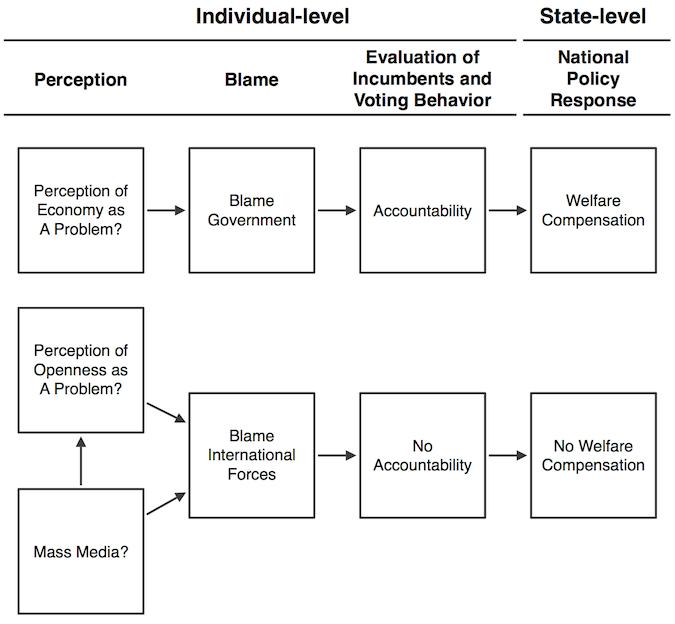
\includegraphics{article1_flowchart}
\caption{Summary of the Hypothesized Effects of Perception and Mass Media in Domestic Responses to Economic Liberalization}
\end{figure}
\end{center}

\section{Data and Method}

Given the individual-level and state-level implications of the theory, data is gathered from both
levels of analysis.\footnote{Full summary statistics for both datasets can be found in the online
appendix.} The individual-level data come from a Legidoscope survey of public opinion in France
between 1992 and 1993 (\citealt{Chrique:1993us}). Around the time of the Maastricht Treaty,
especially controversial in France, the problems of economic openness are likely to be highly
salient. Additionally, France has relatively high rates of voter turnout, and a statist, egalitarian
political culture. Thus, evidence that mass media leads French citizens near the time of Maastricht
to blame international forces rather than their government suggests that such a relationship is at
least as likely in the many countries in which the economy and globalization are less politicized.
Similarly, if mass media pacifies French citizens in either perceptions or political behavior, it is
likely to do so in other countries. The survey asks respondents several questions tapping blame
attribution, media exposure, and political mobilization.\footnote{See the online appendix for the
text of the survey questions.} Respondents are asked to identify their main source of information
from among the following: friends, family, opinion leaders, and mass media. Respondents are also
asked to identify the top two problems facing France, and whether individuals, social institutions,
the government, or international forces beyond government control are to blame for the problem.
\footnote{Respondents were asked to identify national problems in an open-ended fashion; their
answers were then coded by the interviewer and into the general problem types listed here. To create
the binary variable which measures whether the respondent sees some aspect of international economic
openness as a top problem, I coded respondents as 1 if they identified one of the following issues
as one of the ``second most important problems'': ``Int\textquoteright{}l economic competition,''
``EC-92, economic integration,'' ``Foreign trade,'' ``Ratification of Maastricht,'' and ``Maastricht
Treaty.'' All other respondents were coded as 0 for the variable $Openness\: Problem$.} Finally,
respondents are asked about their satisfaction with President Mitterand, how well they think the
government is handling the problem identified by the respondent as a top problem, and their
intention to turnout for the March 1993 elections.

To test the direct and indirect effects of mass media on blame (Hypothesis 1), I estimate two
logistic regression models. The first estimates the probability a respondent will blame
international forces as a function of mass media exposure and a vector of control variables
including controls for the nature of the problem. The equation is

\begin{eqnarray} Blame_{i} & = & \alpha+\beta_{1}General\: Problem\: Type_{i}+\beta_{2}Openness\:
Problem_{i}+\beta_{3}Media_{i}+ \notag \\ &  & \beta_{4}Controls_{i}+e_{i}, \end{eqnarray}

\noindent where $Blame$ is a binary variable taking a value of 1 for respondents who blame
international forces and 0 for respondents who blame the government for whichever national problem
they have identified.% \footnote{Because of space constraints and for ease of interpretation in
light of the hypotheses under consideration, I consider here only the difference between blaming the
government and blaming international forces, omitting respondents who placed the blame on
``society'' or ``people like you and me.'' However, the results obtained here are robust to
multinomial specifications which include these alternative blame attributions and alternative binary
codings (included in the online appendix).% } $General\: Problem\: Type$ is a categorical variable
with four levels indicating whether the problem deals with social, economic, political, or foreign
issues;% \footnote{In the first wave of the survey, so many respondents identified unemployment as
the top problem facing France that a question was added to measure what respondents identified as
the ``second most important problem facing France today.'' All the analyses here, including the
variables measuring blame attributions and evaluations of government handling, refer to this second
most important problem.% } $Openness\: Problem$ is a binary variable I constructed to take a value
of 1 for respondents who identified a problem specifically related to economic openness and 0
otherwise. If the mass media have an independent effect on diffusing blame away from government
policymakers and toward international forces, then we would expect $\beta_{3}$ to be positive and
significant.

Then, to assess the indirect effect of mass media on blame as its channeled through perceptions of
economic openness, I estimate a logistic regression modeling the probability of perceiving openness
as a top problem as a function of mass media exposure and a vector of control variables:

\begin{eqnarray} Openness\:Problem_{i} & = &
\alpha+\beta_{1}General\:Problem\:Type_{i}+\beta_{2}Media_{i}+ \notag \\ &  &
\beta_{3}Controls_{i}+e_{i}. \end{eqnarray}

where the main variables of interest are the same as in Equation 1 except that here the dependent
variable is the binary variable capturing whether openness is perceived as a top problem. If mass
media affect blame attributions indirectly by making individuals more aware of international
economic forces, which in turn would shift their blame toward international forces, then $\beta_{2}$
should be positive and significant.

To test Hypothesis 2 regarding the effect of blame attributions on evaluations of the government, I
estimate a linear regression modeling how individuals evaluate the government's handling of the
problem they identified as one of the most important facing the country. I model evaluations of
government handling as a function of respondents' blame attributions and a vector of control
variables. The equation is

\begin{eqnarray} Gov\:Handling_{i} & = &
\alpha+\beta_{1}General\:Problem\:Type_{i}+\beta_{2}Openness\:Problem_{i}+ \notag \\ &  &
\beta_{3}Blame_{i} + \beta_{4}Controls_{i}+e_{i}, \end{eqnarray}

\begin{doublespace} \noindent where $ $$GovHandling_{i}$ measures, on a scale from 1 to 4, how the
\emph{i}th respondent evaluates the government's handling of the top problem they identified. The
theory predicts that for a particular problem such as the domestic costs of economic openness,
blaming international forces rather than the government will make individuals less likely to hold
governments accountable for that problem. If this is the case, then individuals who think a problem
is caused by forces outside of the government's purview should be less critical of the government's
handling of that problem. In this case, then, the theoretical expectation is that $ $$\beta_{3}$
will be positive and significant, reflecting that blaming international forces for a problem leads
individuals to view the government's handling of that problem more favorably than if they blamed the
government for the problem. \end{doublespace}

\begin{doublespace} To test Hypothesis 3, I estimate a logistic regression modeling the probability
a respondent intends to vote in the March 1993 legislative elections as a function of several
predictors. As the traditional ``compensation'' model suggests, individuals who are dissatisfied
with the domestic consequences of economic openness will take their dissatisfaction to the polls.
According to the compensation perspective, this threat posed by domestic groups harmed by economic
openness accounts for why we observe larger welfare states in countries more exposed to the
international economy. The theory developed here, however, suggests that this threat should be
conditional on whether or not individuals blame government policymakers for economic openness as a
problem. Hypothesis 3 modifies the conventional expectation by predicting that individuals who are
most dissatisfied with economic openness will be less likely to mobilize against a government for
this grievance if they think the cause of their grievance is outside of the government's purview.
Our theory is agnostic about whether or not perceptions of openness as a top problem makes
individuals more or less likely to vote than individuals who perceive some other problem as the top
problem. In other words, testing Hypothesis 3 requires that we consider the behavioral effect of
perceiving openness as a problem and blaming international forces for that problem. Thus, I model
the probability an individual intends to vote as a function of the multiplicative interaction
between perceiving openness as a problem and blaming international forces for that problem:
\end{doublespace}

\begin{eqnarray} Turnout_{i}& =
&\alpha+\beta_{1}GeneralProblemType_{i}+\beta_{2}OpennessProblem_{i}+ \beta_{3}Blame_{i} + \notag \\
&  & \beta_{4}OpennessProblem_{i}*Blame_{i}+\beta_{5}Controls_{i}+e_{i},
\end{eqnarray}$\begin{aligned}\end{aligned} $

\begin{doublespace} \noindent where $Turnout_{i}$ is a binary variable taking a value of 1 for
respondents who report that they intend to vote in the March 1993 legislative elections and 0
otherwise, and $OpennessProblem_{i}*Blame_{i}$ is the multiplicative interaction of the two
respective binary variables. In this equation, the coefficient of interest is the coefficient of the
interaction term, $\beta_{4}$, which we would expect to be negative if blaming international forces
decreases the mobilizing effect of dissatisfaction with openness. \end{doublespace}

To test Hypothesis 4, state-level economic data are gathered from the World Bank's World Development
Indicators (\citealt{WorldDevelopmentIn:2012wl}). Media penetration rates come from the World
Development Indicators and Arthur Banks' Cross-National Time-Series Data Archive
(\citealt{CrossNationalTime:td,WorldDevelopmentIn:2012wl}). Most models have around 130 countries
with an average of roughly 8 observations per country.% \footnote{See online appendix.% } To test
whether mass media affects domestic compensation for globalization at the state level, I fit several
variants of the pooled cross-sectional, time-series regression equation:

\begin{eqnarray} Spending_{it}& =
&\alpha+\beta_{1}Trade_{it}+\beta_{2}MDI_{it}+\beta_{3}Trade_{it}*MDI_{it}+ \notag \\ &  &
\beta_{4}Controls_{it}+e_{it}, \end{eqnarray}

\noindent where the dependent variable, $Spending_{it}$, is a measure of final government
consumption expenditure for country $i$ in year $t$. Final government consumpiton expenditure is a
standard measure of social welfare spending\emph{; Trade} indicates imports plus exports as a
percentage of GDP and \emph{MDI} indicates an additive index of media density measuring television,
newspaper, and radios per capita (\citealt{Camber:2013ul}). Because the theory deals with the
conditioning effects of mass media on domestic exposure to the global economy, I am most interested
in the multiplicative interaction of trade and mass media ($Trade_{it}*MDI_{it}$) rather than the
independent marginal effects. If mass media exposure has the individual-level effects hypothesized
above, then an increasing density of mass media technologies within a state should weaken the
positive relationship historically expected between levels of trade openness and levels of domestic
spending. In other words, the coefficient $\beta_{3}$ should be negative and significant, reflecting
that the predicted effect of trade on spending given high levels of mass media is less than the
predicted effect that trade has on spending given low levels of mass media. In the first models
testing Hypothesis 4, a battery of controls are included to account for non-trade and non-media
determinants of government consumption expenditure. Data for testing particular rival explanations
are significantly more limited and therefore significantly reduce the geographic and temporal
coverage of the main economic and media data. For this reason, I check the robustness of my models
against alternative explanations in a set of subsequent models.


\section{Findings and Discussion}

The coefficient plots in Figures 2 and 3 show statistical support for the expectation that mass
media have both direct and indirect effects on blaming international forces for national problems.%
\footnote{Numerical model results are available in the appendix. All models were estimated with the
Zelig package in R (\citealt{ZeligEveryonesSt:2009ts})} Considering the direct effect of mass
media on blame attributions graphed in Figure 2, respondents who rely on the mass media as their
most important source of information are significantly more likely to blame international forces for
what they identify as one of the nation's top problems (a logit estimate of .35 and standard error
of .12), even controlling for perceptions of economic openness as a problem and the more general
issue area in which a respondent locates that problem. But as we would expect from previous research
on public opinion and voting in open economies, the perception of economic openness as a problem
also increases the probability a respondent will blame international forces for that problem.%
\footnote{It could be the case that individuals with cosmopolitan outlooks are more interested in
mass media \emph{because} of their greater interest in global issues, in which case mass media
exposure could be endogenous to knowledge of issues surrounding economic globalization. Although the
survey data used in this paper provide no measure of overall interest in international affairs, the
analyses below control for the best predictors of cosmpolitanism: education, class, and general
interest in politics. Because these are the best predictors of cosmpolitanism, it is unlikely that a
partial, independent effect of mass media exposure would be spurious due to this particular risk of
endogeneity.} Indeed, of all the variables considered here, the perception of economic openness as
one of the nation's top problems is the strongest determinant of whether a respondent will blame
international forces for that problem (a logit estimate of 1.1 and standard error of .14). In turn,
considering the indirect effect of mass media on blame attributions, reliance on mass media has a
positive and statistically significant marginal effect on the perception of openness as a problem (a
logit estimate of .44 and standard error of .18).

\begin{center}
\begin{figure}
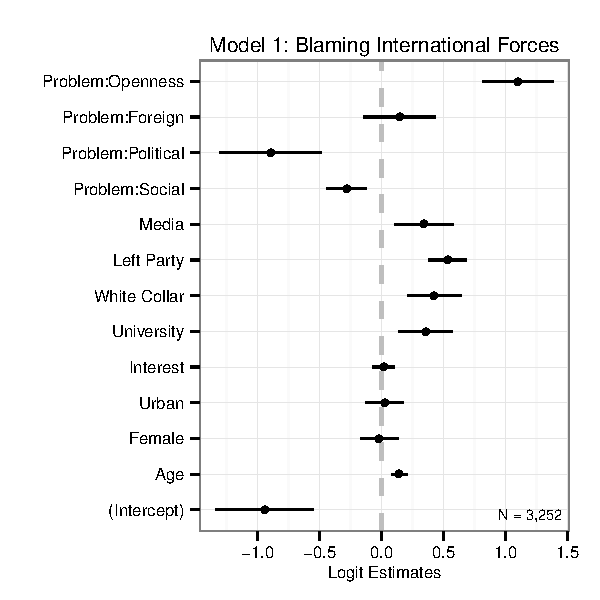
\includegraphics{article1_blame_coefs}
\caption{Direct Effect of Mass Media on Blaming International Forces}
\end{figure}
\end{center}

As logit estimates are not readily interpretable, I simulate the direct marginal effect of mass media on
blame attribution. Figure 4 plots how a typical respondent's main source of information affects the
probability they will blame international forces.\footnote{``Typical'' respondent refers to a
female between the ages of 35 and 49, who is a left-party voter, without a bachelor's degree.}
The effect is small, increasing the probability of blaming international forces by less than one
tenth of a point, but it is statistically distinguishable from zero at a 95\% confidence level.
Similarly, the indirect effect of mass media on blame, through its effects on perceptions of
openness, is only slightly larger than the direct effect.

\begin{center}
\begin{figure}
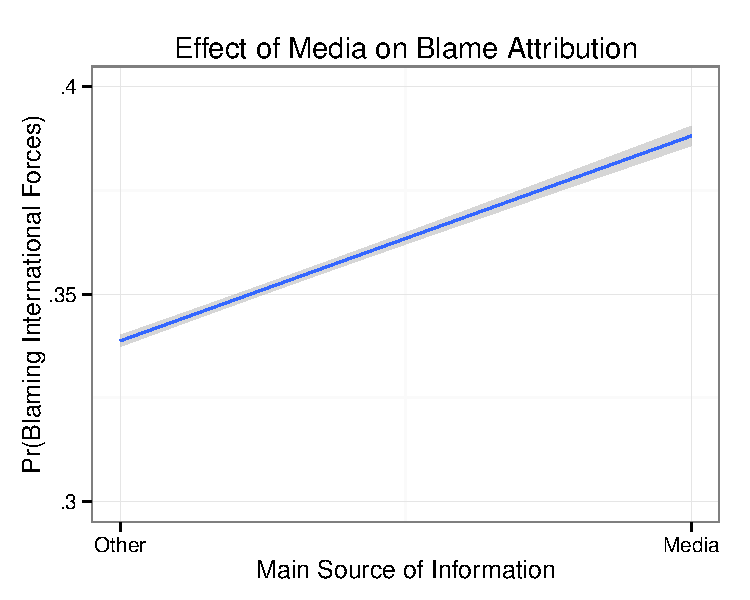
\includegraphics{article1_media_blame_effect}
\caption{Direct Effect of Mass Media on Blame. 95\% confidence intervals in grey.}
\end{figure}
\end{center}

The coefficient plot and simulated probabilities in Figures 5 and 6 reveal statistical evidence for
the expectation that blaming international forces, in turn, has a positive effect on evaluations of
the government.\footnote{There is reason to suppose that blame attributions could be endogenous to
evaluations of how the government is handling a problem, in the sense that poor or satisfactory
government handling could actually increase or decrease the government's culpability. First,
however, it should be recalled that survey question I am using to measure blame attributions refers
specifically to the cause of the problem. Thus, strictly speaking, evaluations of how the government
handles the problem should not affect who or what individuals identify as the cause or source of the
problem. Second, it is much harder to believe that evaluations of government handling could drive
individuals' blame of international forces or blame of the two alternative targets from which
respondents were able to choose (individuals ``like you and I'' or social institutions) simply
because it is hard to imagine how government handling of the problem could make any of these other
targets more or less culpable. Thus, I estimate an additional model which has separate binary
independent variables for blaming government, international forces, or ``other'' as the baseline
(see Online Appendix). The coefficient for blaming government is larger than that for blaming
international forces but both remain signed as expected and significant. This alternative
specification mitigates the possibility that blaming international forces merey reflects
(endogenously) respondents who are less likely to blame the government. Finally, if it can be
assumed that endogeneity between evaluations of handling and blame would be most likely among
partisans, then the control for partisanship and the two separate controls for support of President
Mitterand likely absorb much of this endogeneity.}

\begin{center}
\begin{figure}
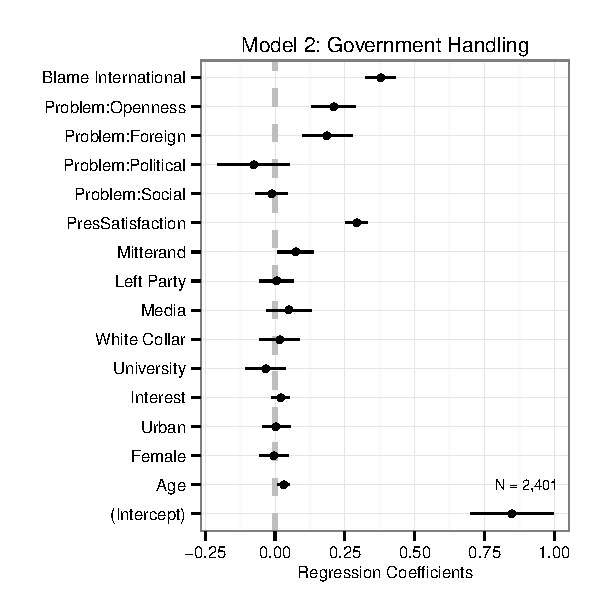
\includegraphics{article1_govhandling_coefs}
\caption{Effects of Blame on Evaluations of the Government}
\end{figure}
\end{center}

Figure 6 shows the simulated effect on evaluations of the government's handling of a problem from
shifting their blame for that problem from the government toward international forces (Hypothesis
2).\footnote{These results also hold when the dependent variable refers to satisfaction with the
President. See appendix.} The typical respondent would be expected to increase their evaluation
of the government (on a four point scale) about .25 points after a shift in blame toward
international forces.

\begin{center}
\begin{figure}
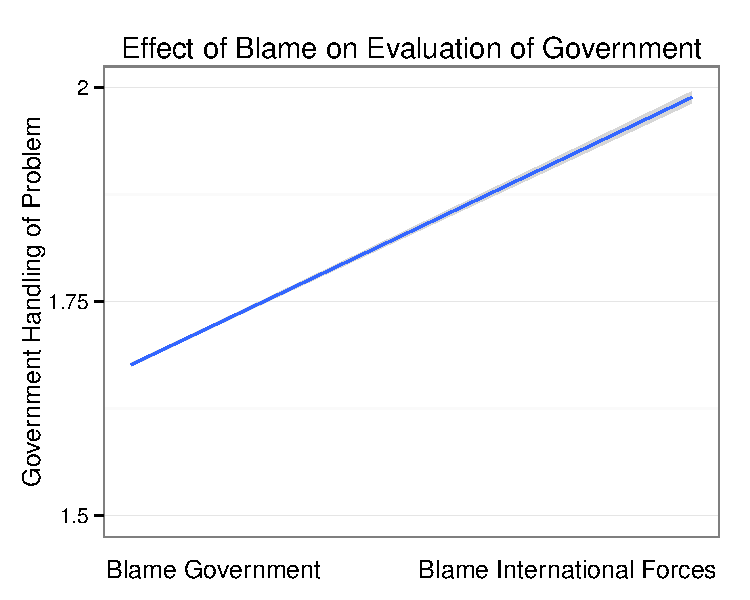
\includegraphics{article1_govhandling_effect}
\caption{Based on 1000 simulations. 95\% confidence intervals in grey.}
\end{figure}
\end{center}

Consistent with the evidence in favor of Hypothesis 2, Figures 7 and 8 suggest evidence for the
predicted, interactive effects of perceptions of openness and blame for openness on voter turnout.
Whereas perceptions of openness as a problem and blaming international forces for that problem both
have positive correlations with voter turnout (only the latter is statistically significant), their
interaction has a negative and statistically significant effect. The logit estimate for the
multiplicative interaction of Problem:Openness and Blame International is .98 with a
standard error of .04. Again, the size of the effect is small, but this is largely because
the unconditional probability that a respondent intends to vote is very high.

\begin{center}
\begin{figure}
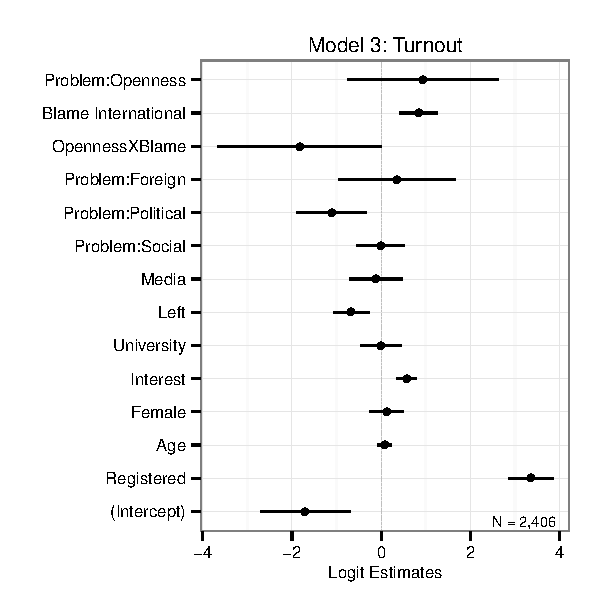
\includegraphics{article1_turnout_coefs}
\caption{The Effect of the Interaction of Openness and Blame on Voter Turnout}
\end{figure}
\end{center}

\begin{center}
\begin{figure}
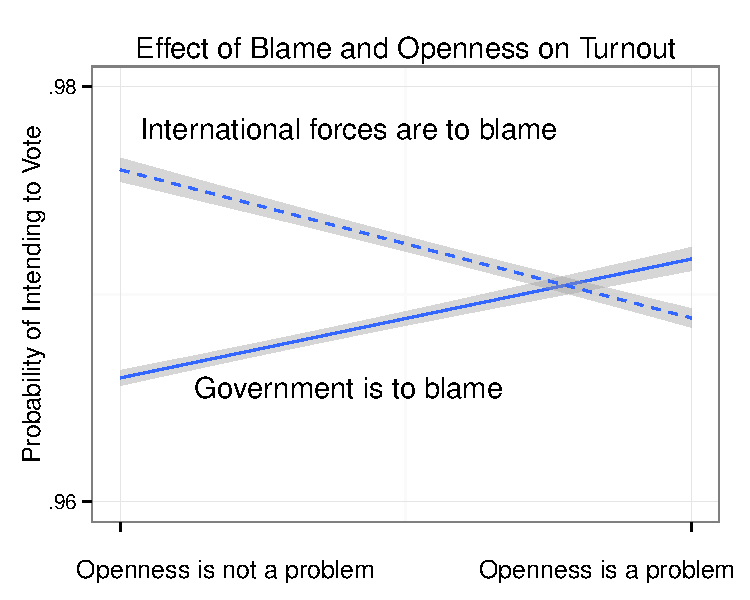
\includegraphics{article1_turnout}
\caption{Based on 1000 simulations. 95\% confidence intervals in grey.}
\end{figure}
\end{center}

Table 1 displays results from three regression models which provide initial support for
the state-level expectations regarding the effect of mass media on the globalization-welfare
relationship. In each of the three model specifications, the variable Trade{*}MDI is negative and
statistically significant, suggesting that media density decreases the effect that trade has on
government consumption expenditure. Before the analysis, all variables were de-meaned and divided by
two standard deviations so that the coefficient for any independent variable can be interpreted as
the expected effect of a two standard deviation increase in that variable. In other words, the
coefficient of -.97 for Trade{*}MDI in Model 1 suggests that, on average, a two standard deviation
increase in media density (109.3 points) in the long-run decreases the effect that a two standard
deviation increase in trade openness (85.2\% of GDP) has on government spending by .97\% of GDP.
Model 3 estimates that this negative conditioning effect of media density is as little as .61\% of
GDP. Moving from the minimum density of media (0) to the maximum in the sample (313.3) is
associated, on average, with a decrease of as much as 2.78\%, and as little as 1.8\%, in the
expected effect of an 85\% increase in trade openness on government spending as a share of GDP.
Although the estimated effect appears relatively slight, it should be kept in mind that the mean
level of government consumption expenditure in the sample is only 15.7\% of GDP. Thus, for a country
that begins with no mass media and becomes as fully penetrated as the most penetrated (the United
States in 1986), the roughly 1-3\% of GDP by which we would expect the country to reduce its
compensatory public spending in the long-run for an 85\% increase in trade openness is a substantial
portion of what a typical country spends.

Models 1 and 2 consider variable levels only, while Model 3 is an error-correction model using
first-differences or year-to-year changes in the dependent variable and lagged levels of the
dependent variable on the right-hand side of the equation, with levels and first-differences of the
key independent variables. Although a level dependent variable with a lagged level on the right-hand
side is formally equivalent to a differenced dependent variable, the error-correction specification
is useful here because it allows us to separate short-run and long-run effects.\footnote{The
error-correction specification is useful here for another reason. Although government spending and
media density are not quite co-integrated, they are nearly cointegrated as both trend upward over
time. In such situations, error-correction specifications are ideal for insuring against the
possibility of spurious correlations driven by that shared integration.} The differenced
independent variables reflect immediate, short-run effects and the level independent variables
reflect the long-run effect after the short-run effects decay. All three models include fixed
effects for country and year to account for unobserved differences in countries or unobserved
temporal shocks in any particular year. To control for the clustering of errors within countries and
the possibility of downwardly biased standard errors, I subsequently calculated panel-corrected
standard errors following Beck and Katz \citeyearpar{Anonymous:DMdF8icE}. Panel-corrected standard
errors did not appreciably change the statistical significance of any estimates reported in this
paper.\footnote{It is common to display the panel-corrected standard errors rather than the
untransformed errors, but it is not obvious that treating them as a default has improved our use of
cross-sectional, time-series data. On this point, see \citealt{Wilson:2007kz}, with whom I take the
view that panel-corrected standard errors are only one of many checks against difficulties common in
cross-sectional, time-series data. Fixed effects, lagged dependent variables, and dynamic
specifications are some of the other techniques stressed by those authors. Here, I employ all of
these techniques, and in some cases all together.}

Columns 2 and 3 test the conditioning effect of media density against the conditioning effects of
democracy on the trade-welfare relationship, which previous research has found to increase the
redistributive responsiveness of domestic welfare spending to international trade
(\citealt{Adsera:2002vt}), suggests that media density has a robust conditioning effect on the
relationship between trade and spending, while the interaction found by Adserà and Boix no longer
appears statistically distinguishable from zero.

\begin{singlespace}
\begin{center}
\def\sym#1{\ifmmode^{#1}\else\(^{#1}\)\fi}
\begin{table}[htbp]
\caption {Determinants of Government Consumption Expenditure} \label{tab:title} 
\centering
\footnotesize
\begin{tabular}{l*{3}{c}}
\hline\hline
  &\multicolumn{1}{c}{spending.wb} &\multicolumn{1}{c}{spending.wb} &\multicolumn{1}{c}{diff(spending.wb)} \\
\hline
lag(trade.wb, 1) 		&0.144 		&0.147 		&0.38\sym{*}\\
  		&(0.213) 		&(0.213) 		&(0.222) \\
lag(mdi, 1) 		&-0.157 		&-0.114 		&0.612\sym{*} \\
  		&(0.402) 		&(0.403) 		&(0.318) \\
lag(polity2, 1) 		&0.025 		&-0.03 		& \\
  		&(0.152) 		&(0.157) 		& \\
lag(gdpcap.wb, 1) 		&0.615\sym{***} 		&0.608\sym{***} 		& \\
  		&(0.189) 		&(0.189) 		& \\
lag(dependency.wb, 1) 		&-0.218 		&-0.235 		& \\
  		&(0.231) 		&(0.232) 		& \\
lag(land.wb, 1) 		&13.921 		&20.356 		& \\
  		&(191.648) 		&(191.676) 		& \\
lag(spending.wb, 1) 		&0.717\sym{***} 		&0.716\sym{***} 		&-0.164\sym{***} \\
  		&(0.016) 		&(0.016) 		&(0.01) \\
lag(spending.wb, 2) 		&0.11\sym{***} 		&0.111\sym{***} 		& \\
  		&(0.016) 		&(0.016) 		& \\
lag(trade.wb, 1):lag(mdi, 1) 		&-0.97\sym{***} 		&-0.883\sym{***} 		&-0.611\sym{*} \\
  		&(0.32) 		&(0.325) 		&(0.317) \\
lag(diff(trade.wb)):lag(diff(mdi)) 		& 		& 		&8.139 \\
  		& 		& 		&(15.681) \\
lag(trade.wb, 1):lag(polity2, 1) 		& 		&-0.428 		&-0.434 \\
  		& 		&(0.303) 		&(0.294) \\
lag(diff(trade.wb)):lag(diff(polity2)) 		& 		& 		&-3.557\sym{*} \\
  		& 		& 		&(1.963) \\
lag(diff(trade.wb), 1) 		& 		& 		&-0.946\sym{**} \\
  		& 		& 		&(0.388) \\
lag(diff(mdi), 1) 		& 		& 		&0.562 \\
  		& 		& 		&(1.716) \\
lag(diff(polity2), 1) 		& 		& 		&-0.056 \\
  		& 		& 		&(0.284) \\
lag(diff(gdpcap.wb), 1) 		& 		& 		&0.668 \\
  		& 		& 		&(0.723) \\
lag(diff(dependency.wb), 1) 		& 		& 		&2.4 \\
  		& 		& 		&(1.794) \\
lag(diff(spending.wb), 1) 		& 		& 		&-0.104\sym{***} \\
  		& 		& 		&(0.016) \\
\hline
$R^2$ 		&0.672 		&0.672 		&0.104 \\
$adj.R^2$ 		&0.638 		&0.638 		&0.098 \\
$N$ 		&\multicolumn{1}{c}{3911} 		&\multicolumn{1}{c}{3911} 		&\multicolumn{1}{c}{3914} \\
\hline\hline
\multicolumn{4}{l}{\footnotesize Standard errors in parentheses}\\
\multicolumn{4}{l}{\footnotesize $^{*}$ (p $\le$ 0.1), $^{**}$ (p $\le$ 0.05), $^{***}$ (p $\le$ 0.01)}\\
\end{tabular}
\end{table}

\end{center}
\end{singlespace}

\subsection{Rival Explanations}

To check for the possibility that the above models are spuriously driven by some different but
unobserved process distinct from the effects of mass media, I gather additional data to test my
arguments against a series of rival explanations. Specifically, it is argued that left parties and
union density are aspects of the domestic institutional environment which lead to more
redistributive responses to economic liberalization (\citealt[674]{Garrett:1995tj}); that electoral
systems defined by proportional representation are more redistributive than majoritarian systems
(\citealt{Iversen:2006wd}); and that the degree of unitarism or government centralization affects
welfare spending (\citealt[72]{Crepaz:1998vj}). Finally, of particular interest in the literature
relating economic globalization to the politics of welfare is the argument of Iversen
(\citeyear{Iversen:2001vr}) and Iversen and Cusack (\citeyear{Iversen:2000ch}) that
deindustrialization rather than globalization has driven the expansion of welfare spending since the
1960s.

In Table 2, I re-estimate the error-correction model (as in Column 3 of Table 1) controlling for
each of the rival explanations above.\footnote{See Supporting Information for more information on
variable descriptions and sources.} The interaction of trade levels and media density levels is
robust to the inclusion of each potentially confounding variable, suggesting that the conditioning
effect of media density on the trade-spending relationship is not a spurious correlation due to an
omitted variable. Rather, the state-level models overall furnish another level of robust evidence
that mass media shape perceptions and blame attributions around economic globalization in a way that
diffuses the domestic political pressure required for compensatory, redistributive policy response.

\begin{singlespace}
\begin{center}
\def\sym#1{\ifmmode^{#1}\else\(^{#1}\)\fi}
\begin{table}[htbp]
\scriptsize
\caption{Rival Explanations: Electoral System, Centralization, Left Party Seats, Union Density, and De-Industrialization}
\begin{tabular}{l*{5}{c}}
\hline\hline
  &\multicolumn{1}{c}{(1)} &\multicolumn{1}{c}{(2)} &\multicolumn{1}{c}{(3)} &\multicolumn{1}{c}{(4)} &\multicolumn{1}{c}{(5)} \\
\hline
lag(diff(trade.wb), 1) 		&-0.668 		&-0.429 		&-2.431\sym{**} 		&-1.362 		&-1.345\sym{***} \\
  		&(0.458) 		&(0.467) 		&(1.055) 		&(0.879) 		&(0.481) \\
lag(mdi, 1) 		&0.045 		&-0.014 		&-0.278 		&-0.589\sym{**} 		&-0.047 \\
  		&(0.416) 		&(0.416) 		&(0.262) 		&(0.242) 		&(0.677) \\
lag(diff(mdi), 1) 		&0.814 		&0.743 		&2.258\sym{***} 		&2.839\sym{***} 		&-0.919 \\
  		&(1.743) 		&(1.741) 		&(0.775) 		&(0.821) 		&(2.253) \\
lag(gdpcap.wb, 1) 		&0.472\sym{**} 		&0.509\sym{***} 		&0.556\sym{***} 		&0.427\sym{***} 		&0.833\sym{***} \\
  		&(0.187) 		&(0.187) 		&(0.137) 		&(0.117) 		&(0.285) \\
lag(spending.wb, 1) 		&-0.233\sym{***} 		&-0.234\sym{***} 		&-0.071\sym{***} 		&-0.075\sym{***} 		&-0.247\sym{***} \\
  		&(0.014) 		&(0.014) 		&(0.018) 		&(0.015) 		&(0.013) \\
lag(trade.wb, 1):lag(mdi, 1) 		&-0.662\sym{*} 		&-0.641\sym{**} 		&-0.891\sym{**} 		&-1.184\sym{***} 		&-1.919\sym{***} \\
  		&(0.342) 		&(0.324) 		&(0.354) 		&(0.314) 		&(0.542) \\
lag(diff(trade.wb), 1):lag(diff(mdi), 1) 		&5.072 		&4.268 		&-39.462 		&-41.014 		&41.667\sym{*} \\
  		&(18.142) 		&(18.194) 		&(25.394) 		&(25.531) 		&(25.254) \\
lag(pr, 1) 		&0.476 		& 		& 		& 		& \\
  		&(0.359) 		& 		& 		& 		& \\
lag(trade.wb, 1):lag(pr, 1) 		&0.296 		& 		& 		& 		& \\
  		&(0.334) 		& 		& 		& 		& \\
lag(diff(trade.wb), 1):lag(diff(pr), 1) 		&-11.343\sym{***} 		& 		& 		& 		& \\
  		&(3.858) 		& 		& 		& 		& \\
lag(unitarism, 1) 		& 		&-0.695 		& 		& 		& \\
  		& 		&(0.681) 		& 		& 		& \\
lag(trade.wb, 1):lag(unitarism, 1) 		& 		&0.651 		& 		& 		& \\
  		& 		&(0.536) 		& 		& 		& \\
lag(diff(trade.wb), 1):lag(diff(unitarism), 1) 		& 		&-12.632\sym{*} 		& 		& 		& \\
  		& 		&(6.579) 		& 		& 		& \\
lag(netden, 1) 		& 		& 		&-0.086 		& 		& \\
  		& 		& 		&(0.167) 		& 		& \\
lag(trade.wb, 1):lag(netden, 1) 		& 		& 		&-0.8\sym{**} 		& 		& \\
  		& 		& 		&(0.393) 		& 		& \\
lag(diff(trade.wb), 1):lag(diff(netden), 1) 		& 		& 		&-14.819 		& 		& \\
  		& 		& 		&(21.369) 		& 		& \\
lag(lefts, 1) 		& 		& 		& 		&0.208\sym{*} 		& \\
  		& 		& 		& 		&(0.125) 		& \\
lag(trade.wb, 1):lag(lefts, 1) 		& 		& 		& 		&0.441 		& \\
  		& 		& 		& 		&(0.343) 		& \\
lag(diff(trade.wb), 1):lag(diff(lefts), 1) 		& 		& 		& 		&-2.568 		& \\
  		& 		& 		& 		&(4.755) 		& \\
lag(industry.wb, 1) 		& 		& 		& 		& 		&0.06 \\
  		& 		& 		& 		& 		&(0.253) \\
lag(diff(industry.wb), 1) 		& 		& 		& 		& 		&-0.862\sym{*} \\
  		& 		& 		& 		& 		&(0.517) \\
lag(mdi, 1):lag(industry.wb, 1) 		& 		& 		& 		& 		&0.495 \\
  		& 		& 		& 		& 		&(0.56) \\
lag(diff(mdi), 1):lag(diff(industry.wb), 1) 		& 		& 		& 		& 		&56.869\sym{**} \\
  		& 		& 		& 		& 		&(25.815) \\
\hline
$R^2$ 		&0.125 		&0.123 		&0.194 		&0.147 		&0.144 \\
$adj.R^2$ 		&0.115 		&0.114 		&0.17 		&0.131 		&0.134 \\
$N$ 		&\multicolumn{1}{c}{2224} 		&\multicolumn{1}{c}{2224} 		&\multicolumn{1}{c}{544} 		&\multicolumn{1}{c}{673} 		&\multicolumn{1}{c}{2736} \\
\hline\hline
\multicolumn{6}{l}{\footnotesize Standard errors in parentheses. For space constraints, estimates for land,} \\
\multicolumn{6}{l}{\footnotesize dependency rates, levels of trade, and democracy are included but not} \\
\multicolumn{6}{l}{\footnotesize displayed (all were indistinguishable from zero at 95\% confidence).}\\
\multicolumn{6}{l}{\footnotesize $^{*}$ (p $\le$ 0.1), $^{**}$ (p $\le$ 0.05), $^{***}$ (p $\le$ 0.01)}\\
\end{tabular}
\end{table}

\end{center}
\end{singlespace}


\section{Conclusion}

This study has presented individual- and state-level evidence that mass media functions as a
political institution which conditions the domestic politics of economic globalization. Because
politicians use mass media to avoid blame, mass media decrease the accountability of national
economic policymakers who pursue liberalization. Survey evidence shows that individuals most reliant
on mass media are less likely to blame incumbent governments for problems wrought by economic
liberalization. Mass media \emph{indirectly} deflects blame away from incumbent governments by
making individuals more aware of economic openness as a political issue, but it also \emph{directly}
decreases individuals' propensities to blame incumbents (controlling for the awareness effect), most
likely due to framing effects inherent in mass media. Cross-sectional, time-series data reveal that
mass media is associated with a decrease in the relationship between economic openness and welfare-
state spending, providing further evidence that mass media diffuses the domestic political pressure
against liberalization that has historically elicited welfare-state compensation for aggreived
domestic groups. The state-level evidence is consistent with the individual-level evidence that mass
media shifts blame attributions away from governments and toward unaccountable international forces,
which in turn allows national economic policymakers to neglect welfare-state compensation of harmed
domestic groups.

%%%%%%%%%% CHAPTER BREAK %%%%%%%%%%%%%%%%%%%%%%%%%%%%%%%%%%%%%%%%%%%%%%%%%%%%%%%

\chapter{Why are the Most Trade-Open Countries More Likely to Repress the Media?}

\section{Abstract}

Why are more trade-open countries more likely to repress the media, even though media freedom is
positively correlated with most other components of economic globalization? To explore and
understand this little-known empirical puzzle, I argue that economic globalization exerts
contradictory pressures on state-media relations. On the one hand, economic openness encourages
national policymakers to promote media freedom because foreign investors are more likely to invest
where information is reliable. On the other hand, because adjusting to economic openness implies
distributive conflict which can threaten the government, openness also generates incentives for
national policymakers to suppress information and communication about the costs of liberalization.
This paper develops a theoretical model that reconciles these contradictory expectations by
disaggregating economic globalization into its component parts and distinguishing changes
(liberalization) from levels of economic globalization (openness). I argue that liberalization of
trade, inward foreign direct investment, and inward capital flows increase the probability states
will repress the media, as states seek to quell domestic conflict around the adjustment costs of
liberalization. In the long run, however, different types of economic openness exert different
pressures on media freedom depending on how much they reward transparency. I argue that financial
openness leads to greater media freedom in the long run because transparency is important to capital
markets, but trade openness exerts no positive effect on media freedom in the long run because
foreign importers and exporters are unaffected by transparency in other countries. To test these
expectations, I use a mixed-methods research design employing large-N statistical tests combined
with process-tracing in Argentina and Mexico.

\section{Introduction}

Given the conventional wisdom that democratic political institutions drive economic openness
(\citealt{Milner:2005ci}) and vice-versa (\citealt{EICHENGREEN:2008gg}), it is surprising that since
the 1960s, on average, those countries which have been more open to international trade have had
lower levels of media freedom. Although international portfolio capital and foreign direct
investment are each positively correlated with media freedom around the world, the bivariate
relationship between trade and media freedom is slightly negative.\footnote{Disaggregated economic
data come from the World Bank Development Indicators (\citealt{WorldDevelopmentIn:2012wl}) and data
on media freedom come from Freedom House () and Van Belle's Global Press Freedom Dataset
(\citealt{van2000press}). See the section on Data and Method below for a more detailed discussion of
data and coding.} Considering the 151 countries between 1960 and 2011 for which there is available
data, those countries which most often had a repressive media environment had higher levels of trade
than those countries which most often had a free media. This is true in democratic and non-
democratic countries, although the negative relationship is weaker in democratic countries. Given
the positive correlation found between media freedom and other measures of economic openness such as
portfolio capital flows foreign direct investment, and the KOF Globalization index
(\citealt{dreher2008measuring}), the coincidence of high trade openness and media repression is a
surprisingly under-reported empirical puzzle in international and comparative political economy.

This puzzle points to a larger gap in research on the domestic effects of economic globalization.
International and comparative political economists have not yet developed a serious theoretical and
empirical account of how a country's media are likely to be affected by that country's integration
into the international economy. Much is known about the effects of economic integration on aspects
of domestic politics such as cleavages (\citealt{Rogowski:1987ip}, \citeyear{Rogowski:1989wm};
\citealt{hiscox2002international}), growth rates (\citealt{Rodriguez:2001uw}); domestic spending
(\citealt{Rodrik:1998te,Burgoon:2001dp}), civil war (\citealt{Barbieri:2005uk,Bussmann:2007vx}), and
generic measures of democracy (\citealt{EICHENGREEN:2008gg,Li:2003vj}), but very little is known
about how economic integration affects state-media relations. One exception is a working paper by
Orion Lewis (\citeyear{Anonymous:lbhrCJXF}), which finds mixed but suggestive evidence that trade
openness is negatively related to media freedom and portfolio capital is positively related to media
freedom. Other research has considered whether political and civil liberties (broadly including
freedom of the media) affect international economic flows (\cite{Adam:2007gn}) and the effect of
media in economic reform (\citealt{Coyne:2004bq,Islam:2002uc}), but in the extant literature there
is no systematic analysis of whether and in what ways domestic media freedom has been shaped by
increasing international economic integration around the world.

\begin{center}
\begin{figure}
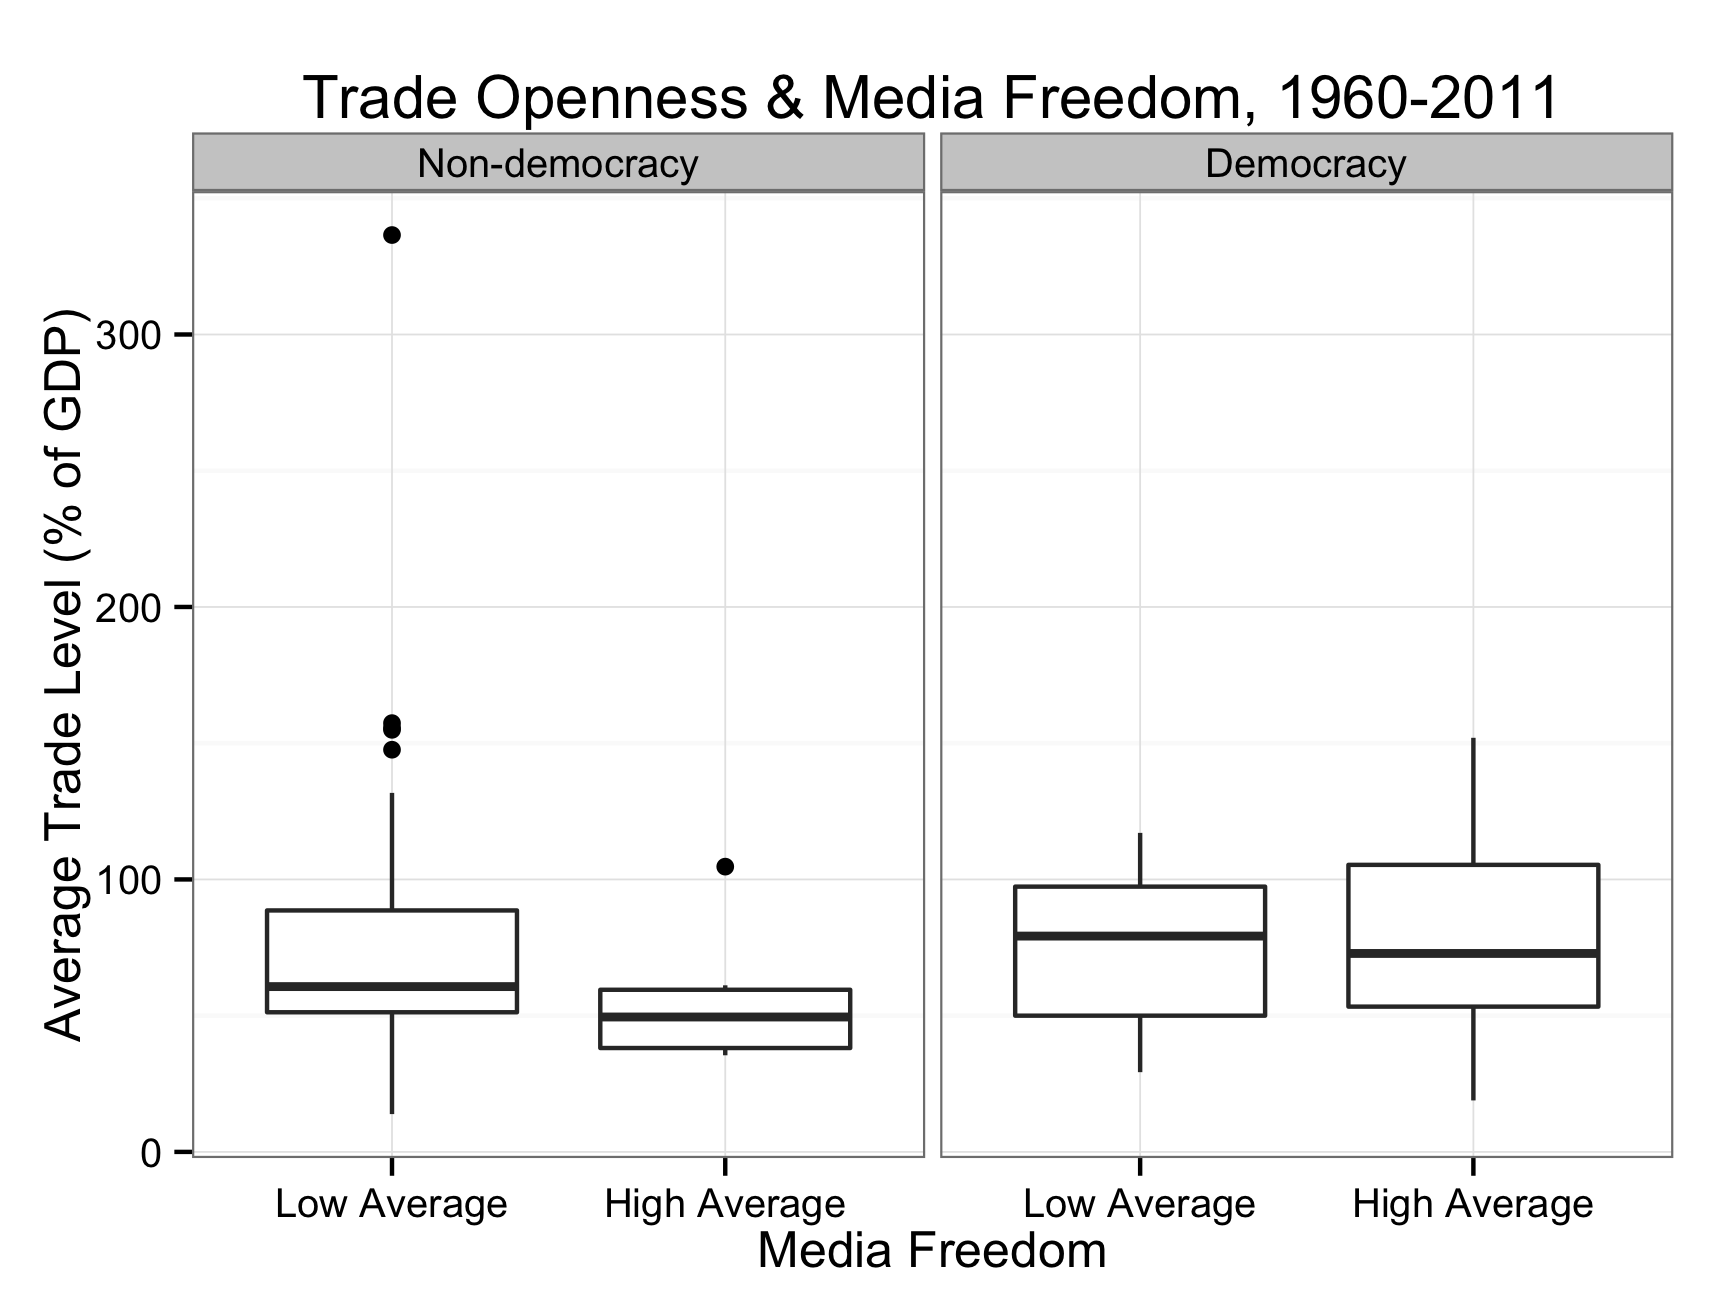
\includegraphics[scale=0.2]{article2_introplot.png}
\caption{Mean Trade Levels and Mean Media Freedom, 1960-2011}
\end{figure}
\end{center}

The present study provides a theoretical account of how different international economic flows
affect domestic media freedom differently, focusing on the puzzling negative correlation between
trade levels and media freedom. It improves on the limited previous research in two ways. First,
Lewis (\citeyear{Anonymous:lbhrCJXF}) uses only the Freedom House measures of press freedom and
therefore considers country-level panel data only between 1993 and 2006. The present study
incorporates the Global Media Freedom Index by Van Belle (\citeyear{van2000press,Belle:1997wo}) to
consider a similar panel of countries for the much longer timeframe from 1960 to 2011. Second, I
emphasize the difference between levels and changes (long-run and short-run effects) in a country's
exposure to international economic flows, whereas Lewis considers only levels.

\section{Globalization, Democracy, and Media}

Previous research provides strong reasons to expect the global integration of markets to exert
pressures on institutions of democracy, but there remains much theoretical uncertainty about the
degree to which these effects are positive or negative. Many have argued that economic globalization
generates economic growth which strengthens democratic institutions (\citealt{Baghwati:1997vy};
\citealt{Im:1996cl}), increases incentives for peace (\citealt{Baghwati:1997vy,Oneal:1999fc}), or
diffuses democracy as a norm (\citealt{Kant:1983uf,Limongi:1996dr}) On the other hand, many have
argued that economic globalization is negatively associated with democracy because it rewards
efficiency rather than popular sovereignty
(\citealt{Huntington:1975vt,Lindblom:1977ue,Cammack:1998gf}), or because leaders may prefer to
repress rather than compensate the domestic losers from increased openness
(\citealt{Adsera:2002vt}).\footnote{See \citealt{Li:2003vj} for a detailed overview of this debate.%
} Within the general debate surrounding the globalization-democracy nexus, some researchers such as
Li and Reveuny (\citeyear{Li:2003vj}) have sought greater clarity by disaggregating the distinct
types of international economic flows and considering them separately, but relying on standard
aggregate measures of democracy. Li and Reveuny find that trade and portfolio capital have negative
effects on democracy, while foreign direct investment and democratic norms have a positive effect,
but their dependent variable of democracy is calculated with the common procedure of subtracting the
Polity autocracy score from the Polity democracy score. Thus, despite much research on the
relationship between economic globalization and democracy, and despite evidence that disaggregation
is fruitful for understanding this nexus of relationships, relatively little is known about how
different international economic flows affect the various institutions which separately constitute
what we know as democracy.

In particular, very little research to date queries whether and how economic globalization shapes
state policies regarding domestic media freedom. One exception is Lewis
(\citeyear{Anonymous:lbhrCJXF}), who finds that FDI inflows are positively associated with press
freedom, trade levels are negatively associated with media freedom, and portfolio capital inflows
have no discernible effect on press freedom. But as a first investigation into this question and as
a largely inductive effort to establish the statistical patterns, the theoretical interpretations of
this article are mostly provisional. Additionally, Lewis considers only levels of trade and year-by-
year inflows of FDI and portfolio capital, whereas recent research shows that the distinction
between flows (year-to-year movements) and stocks (the sum of all previous flows) is crucial in
researching the effects of foreign investment on repression (\citeyear{Sorens:2012hc}). As discussed
above, Antonis and Fillapaois (\citeyear{Adam:2007gn}) consider the effect of civil liberties such
as media freedom on FDI, but not whether FDI affects civil liberties.

However, previous research on the relationship between markets and media more generally provides a
basis for theorizing the relationship between economic integration and media freedom. Broadly, one
tradition argues that the spread of markets and freer media are positively associated
(\citealt{Habermas:1991vg,Islam:2002uc,Islam:2003tu}). However, an opposite tradition suggets that
markets and the logic of profits and efficiency create incentives for authoritarianism
(\citealt{Huntington:1975vt}). With respect to media politics in particular, Gehlbach and Sonin
(\citeyear{Gehlbach:2011ky}) show that larger advertising markets are associated with
nationalization of private media because, they argue, the benefits of state control increase with
the advertising market. If economic liberalization tends to enlarge advertising markets by spurring
economic growth, then liberalization might increase the state's incentives to repress private media
just as it increases incentives to nationalize it. Furthermore, international economic integration
brings the threat of social and political backlashes (\citealt{Bussmann:2007vx}), which require the
state to compensate the domestic losers from globalization (\citealt{Rodrik:1998te}) or,
alternatively, repress them (\citealt{Adsera:2002vt}).

On the other hand, the literature on 'competitive authoritarianism' suggests that increasing
economic interdependence is one of the forces which has increasingly rendered traditional
authoritarian repression unfeasible (\citealt[60, 62]{Levitsky:2002gx}). As a country becomes
increasingly integrated with the world economy, it increases the costs of overt authoritarianism by
increasing the salience of international opinion, increasing the voice of domestic opposition, and
increasing the number of domestic actors affected by international perceptions
(\citealt{Levitsky:2006ex}). For example, Fujimori in Peru in 1992 and Putin in Russia in 1993
failed in their efforts to overtly circumvent the legislature in part due to such international
pressures (\citealt[56]{Levitsky:2002gx}).

International pressures against overt authoritarianism force regimes to adopt formally democratic
institutions such as elections, but often leaves them free to violate human rights and civil
liberties. For example, in the US-Mexico negotiations leading up to the North-American Free Trade
Agreement, Mexican leaders made significant changes to present a front of democracy and respect for
human rights to encourage investors, but there was no specific or formal conditionality which would
have prohibited or even discouraged the repression of civil liberties if necessary.

At the same time, Levitsky and Way highlight the media as one of the four main arenas in which
incumbent governments can contest and subvert international pressures to democratize. Competitive
authoritarian governments may permit a formally independent and relatively free media, as in Peru,
Serbia, Panama, or Nicaragua during the late 1980s and much of the 1990s, while engaging in
alternative, more subtle tactics of repression, such as manipulative adminstrations of the law or
tax code (\citealt[53,58]{Levitsky:2002gx})

While economic integration engenders distributive conflicts which tempt states to repress certain
domestic groups at the same time it disincentivizes certain overt techniques of repression,
governments around the world increasingly engage in strategic, authoritarian interventions into
domestic media politics. Corrales and Westhoff \citeyearpar{Corrales:2006vz} find, for instance,
that authoritarian regimes are more likely to develop television than internet, because television
is more easily controlled. Additionally, many authoritarian regimes welcome the internet but are
actively pursuing techniques of information control and manipulation \emph{on} the internet in a
networked fashion (\citealt{MacKinnon:2011id,Pearce:2012fm}). These findings show that however much
economic integration is making certain forms of repression obsolete, newer and more subtle
techniques of media repression remain both attractive and viable.

\section{Theory and Hypotheses}

As Antonis and Fillapaois point out, and as Lewis also argues, research on the relationship between
globalization and democratic institutions likely shows such contradictory results because different
international economic flows exert different pressures. To build on this idea while advancing the
literature beyond the limitations discussed above, the next section provides a more deductive
account of preicisely why we should expect various types of international economic openness to exert
different effects on media freedom.

Based on the review of previous research regarding the domestic political effects of international
economic flows and the media politics of competitive authoritarianism, I develop a simple, informal
rational-choice model of how state media policy should respond to trade, foreign direct investment,
and portfolio capital flows. Consider a state which experiences a variable increase in some inward,
international economic flow of trade, FDI, or portfolio capital. This increased flow will increase
the income of certain domestic groups and decrease the income of others, according to well-developed
open-economy expectations. The increased economic flow can be thought of as random and exogenous or
the result of conscious state policy such as lowering tariffs. If they are well-informed and
mobilized, a domestic group which experiences a negative income shock from economic liberalization
would demand that the policymaker either close the domestic economy or compensate the group for its
income loss, or else face rebellion. The ``rebellion'' could be electoral if the state is a
democracy or a violent insurgency if the state does not have institutions to facilitate peaceful
change. After experiencing the international shock, the media, if free to do so, would report the
protests of the aggrieved group and its causes, namely, increased national exposure to the
international economy and its conflictual distributive consequences. However, if the media does not
fully report the political context and consequences of the international shock, the group which
suffered an income loss would not threaten rebellion at all. A free media, in other words, are
essential for domestic losers from globalization to exercise power in the domestic politics around
the distributive outcomes of economic globalization. Where there is a free media, domestic losers
from globalization hold policymakers accountable, but where there the media are manipulated by
government, the claims of aggreived groups cannot exact concessions from holding policymakers
accountable. This can be from either not reporting and therefore not informing domestic groups of
the political-conflictual nature of globalization, or from silencing those claims if and when they
are made.

After increased exposure occurs, the policymaker would prefer not to compensate the domestic group
but prefers compensation to facing rebellion or closing the economy to \textit{ex ante} levels. The
policymaker can close the political process to any competitors to obviate the political pressure to
compensate them (\citealt{Adsera:2002vt}), but the higher their level of integration, the more
costly are overt types of repression (\citealt{Levitsky:2002gx}). Supposing that a policymaker can
choose among compensating the aggrieved domestic group, excluding competitors from the political
process, or engaging in some repressive practices which vary on a continuum from overt to covert. In
effect, we can conceptualize their utility function as including a penalty on overtness which
increases with the country's economic integration, such that there is decreasing utility to overt
forms of repression such as outright exclusion from the political process or government killings but
this disutility approaches zero for repressive tactics which are relatively obscure such as the
selective prosecution or financial targeting of opponents.

Among the less visible ways of exercising anti-democratic control, information-communication control
will be uniquely attractive for the policymaker. This is because not only are repressive media
tactics less severe than mass killings or canceling elections, but because control of the media
could potentially tame international judgments independently by shaping what gets reported
internationally. That is, control of the media can first minimize policymaker accountability for the
adjustment costs of liberalization by suppressing domestic dissent, but policymakers could also
reasonably expect that suppressing information at home would decrease the flow of negative
information abroad, promoting their international image in part by repressively shaping their image
at home. In summary, increasing linkages to other states and international pressures raise the cost
of overt repression for liberalizing states, which increases the attractiveness of more subtle,
lower-visibility tactics for suppressing dissent against liberalization. Repression of the media
stands out as a uniquely attractive first because it is precisely such a relatively low-visibility,
low-salience type of repression but also because if successful it would tend to lower negative
visibility in general.

\subsection{Differences among trade, foreign direct investment, and portfolio capital}

The previous subsection argues that media repression is uniquely attractive to incumbents presiding
over economic liberalization. However, the international actors who are the counterparties to a
country's international exchanges are also strategic actors. When a government represses the flow of
information and communication within its territory, these counterparties will respond strategically
depending on how their particular investment in the country is affected by domestic freedom of
information and communication. Given that these international counterparties have very different
stakes in domestic media freedom depending on whether they are engaged in trade, foreign direct
investment, or portfolio capital investment, the utility of media repression during economic
liberalization will be conditioned according to a country's composition of exposure to these flows.

\subsubsection{FDI}

FDI is defined as the private capital flows from one firm to an enterprise located in a country
outside of the firm's home nation. FDI flows consist of equity capital, intercompany debt, and
reinvested earnings, whenever the investment is sufficient to give the firm a controlling stake
(typically 10\%) in the enterprise (\citealt[9]{DirectInvestmentTechnicalExpertGroupDITEG:2004wa}:
\citealt[588]{Jensen:2003to}) Foreign direct investment is unique among other types of international
investment in that FDI involves a longer-term committment and thus the interests of FDI investors
are relatively more aligned with the long-term interests of host countries (\citealt{Lipsey:1999tn};
\citealt[588]{Jensen:2003to}). The standard economic theory of FDI suggests that firm-level
investment decisions to invest directly in a foreign country are not based on relative factor
endowments or comparative rates of return, but on domestic market imperfections which can be
exploited by multinational corporations (MNCs) better than domestic firms (\citealt{Hymer:1960vo};
\citealt{dunning2013international}). The distributive consequences of FDI inflows are complex: FDI
is typically thought to increase inequality between skilled and unskilled workers as MNCs tend to be
technologically skill-biased relative to domestic firms (\citealt{Feenstra:1997kx}) and unskilled,
subsistence farmers do not have the resources to become entrepreneurs (\citealt{Basu:2007ir}).
However, FDI is also thought to decrease overall domestic income inequality as an increase in the
supply of capital relative to labor increases wages and reduces inequality between capital and
skilled labor (\citealt{Jensen:2007fr}). Jensen and Rosas present evidence that, because poor
countries have relatively little skilled labor, FDI's effect on closing the gap between skilled
labor and capital is likely to decrease inequality on net even if it increases inequality between
skilled and unskilled labor. Thus, FDI inflows generate distributive conflict among skilled and
unskilled labor, but are unlikely to generate highly salient distributive conflict overall. This
expectation is borne out by research on the relationship between economic globalization and civil
war. Bussmann and Schneider (\citeyear{Bussmann:2007vx}) find, contrary to their expectations, that
inflows of FDI decrease rather than increase the likelihood of civil war onset.

Most significantly, of the three types of international economic actors considered here, investors
of FDI have a long-term stake in the conditions of a host country. Because of this, despite long-
standing expectations that foreign direct investors prefer the efficiency of authoritarian regimes,
the balance of evidence suggests that democracies draw greater FDI flows than autocracies because
they are more credible (\citealt[588]{Jensen:2003to}). Some scholars have sought to extend this
logic by arguing that FDI should be attracted to respect for human rights (\citealt{Blanton:2007ep})
have faced problems of measurement and missing data (\citealt{Sorens:2012hc}). After accounting for
these issues, Sorens and Ruger find no link between FDI and human rights. Thus, while formal
democracy attracts FDI and FDI does not appear to generate intense distributive conflicts, neither
does it appear to ``punish'' governments for violating human rights.

Interestingly, Antonis and Filipaios find, consistent with Jensen, that FDI seeks strong political
rights while its attraction to civil rights is hump-shaped such that FDI is associated with both
high and low levels of civil rights (\citeyear{Adam:2007gn}). One possible explanation of these
inconsistencies is that the socially positive consequences of FDI (rewarding democracy and rule of
law and decreasing civil war onset) occur at the same time as, or perhaps in part through, the
repression of civil rights. This is consistent with the model presented above, wherein the
repression of a particular civil right (the freedom of expression) embodied in media freedom is
repressed to dampen the disruptive effects of new FDI inflows, but in the long run equilibriates to
a high level alongside political rights.

Thus, as argued in the previous section, increases in FDI should be associated with media
repression, but in the long run FDI should be associated with media freedom. Because FDI is not
averse to violations of rights per se, and is perhaps attracted to governments with low respect for
civil rights, governments will use media repression to suppress distributive conflicts associated
with FDI, but after the adjustment takes place and threat of conflict subsides, then FDI in the
long-run should be associated with media freedom for the same reasons it is associated with
democracy, namely credibility and stability.

\subsubsection{Portfolio capital}

Portfolio capital is defined as the purchase of stocks and bonds of less than 10\% of the
outstanding stock of foreign firms (Kenen 1994, Walther 1997). The standard economic theory is that
portfolio capital tends to flow where the rate of return on the target country's domestic assets is
high relative to the riskiness of the investment (\citealt[743]{mosley2003global};
\citealt[685]{ISQU:ISQU420}). Portfolio capital is distinguished by its short-term, speculative
nature compared to FDI. In a benchmark study of how portfolio investors evaluate political risks,
Bernhard and Leblang (\citeyear{Bernhard:2002gy}) show that portfolio investors respond to changes
in country's political system (such as elections), but not to the substance of those changes (for
instance, partisanship). Brooks and Mosley (\citeyear{Brooks:2007we}) show that portfolio investors
do respond to the substance of policymaking, such as partisanship and macroeconomic priorities, but
only in low-information environments such as electoral turnovers. The effects of partisanship and
macroeconomic policy on portfolio capital decrease when the political system itself is stable. The
overall point is that portfolio investors are first and foremost interested in stability and
predictability rather than particular policies, which only matter in periods when the predictability
of the future is low.

Portfolio capital inflows tend to appreciate the domestic currency, which makes imports relatively
cheaper in the home market and exports relatively more expensive to foreigners. This will harm
exports, leading possibly to unemployment or decreases in wage levels in export-intensive
industries. It will also make it harder for domestic firms to compete with relatively cheaper
imports, also possibly leading to unemployment or wage decreases. Finally, cheaper capital imports
can encourage skill-biased shifts in technology usage, increasing the incomes of skilled labor and
decreasing the incomes of unskilled labor (\citealt{Cragg:1996iy}; \citealt{Ros:2000vy}). Finally,
because portfolio capital is relatively liquid, the threat of sudden withdrawal by international
investors is well-known to have highly negative macroeconomic effects, such as in Mexico in 1995 and
Argentina in 2001.

Given the interests of governments and portfolio investors, governments should be inclined to
repress the media in response to the distributive effects of portfolio capital for two reasons.
First, inflows of portfolio capital will make governments more beholden to the prevention of
systemic political risks such as general strikes, expropriations, or revolutions
(\citealt{Clark:1997jg}). This is consistent with anecdotal evidence of portfolio investors who
prefer governments to repress social unrest. Neoliberal economic reforms including international
liberalization are often followed by large increases in foreign portfolio capital, and there is
anecdotal evidence that in some cases foreign investors demand repression explicitly, such as when
Chase Bank's Emerging Markets Group circulated a memo urging Mexican President Ernesto Zedillo to
``eliminate the Zapatistas'' and their uprising in Chiapas in 1994 (\citealt{Silverstein:1995wc}).
Second, given that policy is evaluated by foreign investors largely in light of what is already
known about the government and its history, incumbents who preside over financial liberalization for
that very reason are likely to be sufficiently trusted by foreign capital that relatively subtle
tactics such as media repression would be unlikely to shake confidence, especially if it is in the
interest of preventing larger disruptions such as rebellions. It may be objected that portfolio
investors would dislike media repression because they rely on a reliable flow of information
regarding the country's conditions, but through modern ``news management'' politicians can practice
a highly nuanced kind of transparency for international observers and also seek to repress domestic
media using underhanded tactics. Indeed, country's which are open enough to receive capital inflows
are likely to already be relatively transparent in the ways most relevant to investors, and this
transparency required to induce investment might even embolden the assertiveness of domestic media.%
\footnote{This appeared to happen in Mexico during the 1980s and 90s (\citealt{lawson2002building})%
} Portfolio investors can typically rely on international news sources which are less likely to be
targeted within the host country (on account of their financial independence and being linked to
another sovereign, such as that one in Argentina). Finally, portfolio investors often have access to
private, elite channels which provide them with politically important information about foreign
country conditions before it would even be reported by free media (\citet{Dube:2011uv}).

Thus, we should expect media policy to respond to inflows of portfolio capital just as it responds
to FDI inflows. As a country adjusts to the destabilizing distributive effects of international
portfolio investment, governments will be more likely to repress the media as a relatively discreet
tactic of pacifying social unrest, consistent with investors' interests in stability. However,
inflows of portfolio capital will in the long-run be associated with media freedom, as portfolio
investors prefer high-information environments \emph{ceteris paribus}.

\subsubsection{Trade}

Trade, defined simply as imports plus exports as the percentage of a country's gross domestic
product, is unique among the previous two components of economic globalization in that the
international counterparties have no direct economic stake in the social and political conditions of
the home country. Put simply, trade is not an investment as are FDI and portfolio capital flows. The
standard economic intuition explaining trade flows, although many sophisticated variations and
extensions have been developed, is still the well-known Ricardian theory of comparative advantage.
Other things equal, countries will tend to specialize in producing for export those goods which they
are most advantaged in producing, and import from foreign producers those goods which domestic
producers are unable to produce as efficiently.

International trade theory and much research in political science provides well-established
expectations regarding the distributive effects of a country increasing its exposure to
international trade. The standard Stolper-Samuelson model (\citeyear{Stolper:1941vp}) expects that
increasing trade openness increases the income of the domestically abundant factor while decreasing
the income of the domestically scarce factor. Thus, in capital-rich countries (industrialized or
post-industrial countries), increasing trade openness benefits capital and harms labor, whereas in
capital-poor countries increasing trade openness is expected to benefit labor and harm capital
owners. In his benchmark study on the political consequences of these distributive expectations,
Rogowski (\citeyear{Rogowski:1989wm}) finds strong evidence that domestic political coalitions are
empowered and disempowered by international trade as the Stolper-Samuelson model predicts. Hiscox
(\citeyear{hiscox2002international}) further refines these expectations by showing that history is
more finely explained by distinguishing the relative mobility of factors: when domestic factors are
relatively immobile within the domestic economy, we do not observe class-based cleavages but rather
sector-based cleavages and cross-class alliances, as immobility weds the interests of labor and
capital to their shared industry. In turn, the threat of distributive conflict from international
trade has been found salient enough to explain domestic political outcomes as diverse as the size of
welfare states (\citealt{Cameron:1978vb}; \citealt{Burgoon:2001dp}) and the onset of civil wars
(\citealt{Bussmann:2007vx}).

The international counterparties to a country's international trade have a uniquely low stake in the
political stability of the country, for the simple reason that the import and export of goods and
services is not directly affected by the sanctity of civil rights such as freedom of expression or
media freedom. Although emerging international norms of ``corporate responsibility'' and ``fair
trade'' are increasingly visible in marketing for consumers in the wealthy democracies, these norms
revolve around specific labor market issues such as child labor, ``sweatshops'', and wages paid to
workers in developing countries (\citealt{Moore:2004gy}). Even if some consumers in the wealthy
democracies are increasingly willing to pay for more humane production conditions in foreign
countries (effectively an international tax on repressive production conditions), there is no
evidence and little reason to believe that economic behavior in importing or exporting goods and
services anywhere in the world is in any way responsive to the sanctity of significantly less
salient civil rights such as media freedom. For instance, consumers in the global North may very
well prefer to pay premiums for coffee explicitly labeled as ``fair trade,'' but this provides no
reason to expect they would pay more or less depending on whether the exporting country's trade
agreements were facilitated by media repression. Similarly, if exporters in one country benefit from
lowered tarrifs in a foreign country, compared to FDI and portfolio investors, they have uniquely
less at stake in the political consequences faced by the foreign country with rising imports.

Thus, as with FDI and portfolio capital, we expect changes in trade openness to be associated with a
higher probability of media repression, but unlike FDI and portfolio capital, we expect this effect
of trade liberalization to persist into the long run, as governments face no pressure from their
counterparties to eventually transition to a free media environment. If true, this would explain the
puzzlingly negative correlation between international trade and media freedom despite the positive
association between trade and most other components of economic globalization.

\subsection{Hypotheses}

To summarize, the hypotheses of the preceding subsections can be stated concisely as follows.

H1: Levels of trade openness decrease media freedom.

H2. Levels of portfolio capital increase media freedom.

H3. Levels of foreign direct investment increase media freedom.

H4. Changes in trade, equity, and FDI decrease media freedom.

\section{Data and Method}

To assess the theory, this article pursues a mixed-method research design employing large-N
statistical tests and qualitative within-case analysis on two historically important cases. The
intuition behind this research strategy is that statistical analyses are necessary to disentangle
the independent effects of each economic flow, especially in distinguishing between short-run and
long-run effects, while qualitative analysis is necessary for establishing the existence of a causal
process.

In the quantitative analyses, I use state-level economic data from the World Bank
(\citeyear{WorldDevelopmentIn:2012wl}) for the main independent variables of interest (FDI,
portfolio capital, and trade) for all available countries between 1960 and 2010. For the dependent
variable, I use the well-known Freedom of the Press scores from Freedom House (CITATION) as well as
the the Global Media Freedom Database Van Belle (\citeyear{Belle:1997wo,van2000press}). Freedom
House measures press freedom on a continuous scale from 0 to 100 and covers most countries from 1994
to the end of the economic time-series, whereas Van Belle's data is essentially a dichotomous
measure of media freedom (footnote: it reduces to that) and covers most countries from 1948 to 1995.
To maximize the sample, I create a single measure of press freedom which converts the Freedom House
scores for 1994-2010 to Van Belle's dichotomous scale by interpolating from the two years for which
there are observations on both measures.% \footnote{Specifically, I fit a logistic regression of the
dichotomous variable on the continuous variable for the three years of overlapping observations,
1994-1996. Then for each year post-1995, I imputed to each each country a 1 on the dichotomous scale
for each year their value on the continuous scale had greater than or equal to a .5 probability of
being classified by the model as 1 (roughly all values greater than about 61 on the 100-point
scale), and I gave them a 0 otherwise.% } This operation is somewhat inefficient (information is
lost from the continuous measure) and biased (for some countries it generates artificial ``changes''
in value between the two time periods) but it credibly and consistently extends the time series for
most countries and represents the most spatially and temporally extensive single measure of media
freedom available. Thus, I employ it for the primary analyses but then model and account for
possible spurious ``effects'' due to this operation. To distinguish the separate effects of
different economic flows on media freedom across countries and over time, I use a series of cross-
sectional time-series regression techniques and robustness checks, including panel
vectorautoregression to check against reverse causality.

To corroborate the quantitative findings and enhance our understanding of the key puzzle motivating
this paper, a following section offers two within-case analyses which trace the process whereby
trade liberalization exerts pressure on domestic media freedom. To help control for confounding
spatial and temporal factors, I consider two ``third-wave'' democracies from the same region in the
same time period, Argentina and Mexico in the period between 1990 and 2011. These countries are
analytically well-suited for further examination because they both democratized beginning in the
1980s and were consolidating in the 1990s. In autocratic regimes, even if we observed instances
where media repression follows economic liberalization, it would be hard to infer that
liberalization caused media repression because the media repression could be a function of auotcracy
in general. On the other hand, if media repression follows economic liberalization in countries
which are otherwise politically liberalizing, it will be more credible to infer that possibly
economic liberalization generated the tendency to media repression. Indeed, Argentina and Mexico are
least likely cases to expect media repression at this time because Argentina's Carlos Menem and
Mexico's Carlos Salinas were championed by American politicians as models of democratic economic
liberalization. Latin America is also a substantively attractive region for further study because
Latin America is typically considered the first region where democracies were able to implement
politically difficult ``stabilization'' policies. In the 1970s, it was a puzzle how economic
liberalization would ever be achieved in democratic settings, given the status quo bias of elected
politicians and the popular support for protectionist policies. An implication of this paper's
argument, however, is that even in formally democratic countries economic liberalization may in some
cases induce anti-democratic tactics such as media repression. If this is argument is correct, then
substantively it would be most rewarding to better understand these cases which the conventional
wisdom holds to be democratic sucess stories. Finally, Mexico, unlike Argentina and many other Latin
American countries, did not experience a deeply repressive military junta in the twentieth century.
Thus, if it is plausible that a government's historical legacy of repression could alone make media
repression in a later period more or less likely, then we can be confident this is not an unobserved
variable generating outcomes in both Mexico and Argentina.

Specifically, I offer two short, ``disciplined-configurative'' case studies for the purpose of
better understanding these historically important cases and to further test for the presence of a
causal process (\citealt[75]{george2005case}). I use a combination of structured, focused comparison
and process-tracing, asking specific questions about the hypothesized process in each case and
weighing the empirical results against what the theory expects. Specifically, I ask the following
three questions. What was the policy background as well as the magnitude and timing of trade
exposure? What was the magnitude and timing, if any, of social unrest and was it observably in
response to the distributive effects of trade? What was the magnitude and timing, if any, of
government efforts to restrict freedom of the media? After investigating the historical record, I
outline the answers to these questions and discuss how well they fit the theoretical model.

\section{Analysis}

Table 1 displays the results of 5 different logistic regressions assessing the probability of
observing media freedom in countryit. The model results provide fairly strong evidence that levels
of trade and portfolio capital inflow have opposite long-run effects on media freedom as predicted
in Hypotheses 1 and 2. The results provide no evidence for any relationship between foreign direct
investment and media freedom as predicted in Hypothesis 3, however. Finally, as expected by
Hypothesis 4, the data reveal negative correlations between economic liberalization and media
repression for each type of openness, although none of these estimates are reliable at any greater
than an 80\% confidence level (in the case of trade liberalization).

Model 1 is a baseline model which predicts media freedom simply as a function of democracy, GDP per
capita, and lagged levels of media freedom. The model correctly predicts the state of media freedom
in most country-years. Model 1 correctly predicts 98\% of country-years in which media are repressed
(incorrectly classifying 47 cases out of 2,027) and 96\% of cases in which the media are free
(incorrectly classifying 57 out of 1,432). Considering the logit estimates in terms of probability
rather than log-odds, ceteris paribus, for a country which shifts from full autocracy to full
democracy the probability of observing media freedom is expected to increase 33\% from .11 to .44.
The effect of a two-standard-deviation increase in GDP per capita (from a mean of \$6,359 to
\$24,097), ceteris paribus, increases the probability of observing media freedom 34\% (from .33 to
.67).

Model 2 adds the openness variables to Model 1. Both trade and portfolio capital are signed as
expected and significant at the 95\% level, consistent with the expectations of Hypotheses 1 and 2.
FDI has no statistically discernable effect. Although the model furnishes some evidence that higher
trade levels are associated with media repression and higher portfolio capital flows are associated
with media freedom, Model 2 classifies the observed outcomes exactly as well as Model 1. Thus, while
Model 2 is meaningful as an initial test of the theoretical claims outlined above, it does not
substantively improve our ability to predict variation in media freedom.

Comparison of Model 3 and Model 4 represents a similar exercise as in Models 1 and 2, but using an
error-correction specification (levels and changes of all independent variables) with natural cubic
splines of time instead of a lagged dependent variable. (\citealt{Beck:1998wg}).% \footnote{Because
BTSCS data are essentially grouped duration data, a lagged dependent variable on the right-hand side
of the equation has a much more ambiguous meaning than it does for a continuous outcome variable.
Following Beck 2011 289, if a state has a high propensity to free (or repress) the media at t-1 but
does not, it is unclear whether this should be interpreted as increasing or decreasing its
propensity at time t. Models 1 and 2 include a lagged dependent variable as a harder test for the
possibility that the coefficients of interest are driven by duration dependence, but the prevailing
best practice is the use of splines as suggested by Beck et al. Finally, my efforts to explore a
lagged dependent variable in Models 3 and 4 was barred by overfitting.% } Model 4 provides
additional support for the theory that trade levels exert a negative effect, and portfolio capital a
positive effect, on media freedom. Both are statistically significant at the 90\% level, controlling
for both levels and changes in democracy and GDP per capita. As in Models 1 and 2, accounting for
openness does not strongly alter our ability to predict outcomes in the sample. Whereas Model 3
incorrectly classifies 203 country-years of media repression, Model 4 improves this classifcation by
incorrectly specifying 195 cases. On the other hand, Model 3 incorrectly classifies 215 cases of
media freedom and Model 4 incorrectly specifies 230. However, the signficance of the openness
coefficients suggests that the relatively similar substantive predictions from Models 3 and 4
reflect that historically media freedom is perhaps overdetermined by openness, democracy, and
economic growth. In other words, although Models 3 and 4 do not offer many different predictions in
particular cases, the results nonetheless suggest that any historical interpretation of media
freedom which sees it as merely a function of democratization or modernization would be imputing to
these factors causal effects some portion of which is possibly due to international economic
openness.

Model 4 also presents suggestive but inconclusive evidence for Hypothesis 4 regarding the negative
effect of economic liberalization. The negative coefficients for each differenced variable are
consistent with the expectation that all types of economic liberalization induce media repression in
the short-run, although none of these estimates are statistically significant. However, if all types
of liberalization induce media repression and all types of liberalization are correlated with each
other, then the data could be insufficient for the model to parse even real indepedent effects.
Model 5, then, replaces the liberalization variables with the simple sum of the three. As expected,
the standard error is significantly smaller, statistically significant at an 88\% confidence level.
Although the standard error is larger than the conventional cut-off for statistical significance
(and other resulst reported above are similarly around the 90\% confidence level, less than the
conventionally prefered 95\%), the difference between 95\% and 88\% is itself of dubious
significance. In my own view, given that the research design includes a qualitative component which
will offer independent and alternative evidentiary weight, confidence levels near 90\% are high
enough that we should not yet fail reject the null hypothesis.

\subsection{Effect Sizes}

Based on Model 5, the probability of observing media freedom in a country completely closed to
international trade is .48 holding all the other variables at their means. Moving to the mean level
of international trade in the sample (71\% of GDP) decreases the expected probability of media
freedom by .9. The probability of observing media freedom in the most trade-open countries (greater
than 200\% of GDP) is roughly 23\% less probable than in a trade-closed economy.

The probability of observing media freedom in a country completely closed to portfolio capital is
.36 holding all the other variables at their means. Moving to the mean level of portfolio capital in
the sample (.05\% of GDP) increases the expected probability of media freedom by only .03. But the
probability of observing media freedom in the countries most open to portfolio capital (greater than
5\% of GDP) is roughly 60\% more probable than in a hypothetical country completely closed to
portfolio capital.

\begin{centering}

\begin{table}
\begin{tabular}{lD{.}{.}{3}@{\hspace{2em}}D{.}{.}{3}@{\hspace{2em}}D{.}{.}{3}@{\hspace{2em}}D{.}{.}{3}@{\hspace{2em}}D{.}{.}{3}} \toprule 
 &  \multicolumn{ 1 }{ c }{ (1) LDV } & \multicolumn{ 1 }{ c }{ (2) +Openness} & \multicolumn{ 1 }{ c }{ (3) Spline } & \multicolumn{ 1 }{ c }{ (4)+ Openness} & \multicolumn{ 1 }{ c }{ (5)$X_{it}$ + $\Delta X_{it}$ } \\ \midrule
 (Intercept) & -3.691 ^*   & -3.287 ^*   & 41.520      & -71.072     & -48.327    \\ 
            & ( 0.129 )   & ( 0.148 )   & ( 42.089 )  & ( 109.662 ) & ( 125.215 )\\ 
lpolity2    & 1.800 ^*    & 1.726 ^*    & 4.381 ^*    & 4.372 ^*    & 4.436 ^*   \\ 
            & ( 0.207 )   & ( 0.256 )   & ( 0.484 )   & ( 0.508 )   & ( 0.524 )  \\ 
lgdpcap     & 1.066 ^*    & 1.624 ^*    & 1.847 ^*    & 2.594 ^*    & 2.491 ^*   \\ 
            & ( 0.146 )   & ( 0.225 )   & ( 0.429 )   & ( 0.413 )   & ( 0.418 )  \\ 
lfp         & 6.355 ^*    & 5.868 ^*    &             &             &            \\ 
            & ( 0.209 )   & ( 0.237 )   &             &             &            \\ 
ltrade      &             & -0.520 ^*   &             & -0.466 ^+ & -0.468 ^+    \\ 
            &             & ( 0.179 )   &             & ( 0.270 )   & ( 0.283 )  \\ 
lfdi.in     &             & -0.262      &             & 0.179       & 0.131      \\ 
            &             & ( 0.220 )   &             & ( 0.162 )   & ( 0.221 )  \\ 
lportfolio  &             & 2.191 ^*    &             & 1.533       & 2.203 ^+     \\ 
            &             & ( 0.771 )   &             & ( 0.991 )   & ( 1.334 )  \\ 
splinedf    &             &             & -0.021      & 0.036       & 0.024      \\ 
            &             &             & ( 0.021 )   & ( 0.055 )   & ( 0.063 )  \\ 
splinedf'   &             &             & -0.034      & -0.082 ^+   & -0.074     \\ 
            &             &             & ( 0.023 )   & ( 0.044 )   & ( 0.049 )  \\ 
trade.d     &             &             &             &             & -0.121     \\ 
            &             &             &             &             & ( 0.093 )  \\ 
fdi.in.d    &             &             &             &             & -0.050     \\ 
            &             &             &             &             & ( 0.117 )  \\ 
portfolio.d &             &             &             &             & -0.428     \\ 
            &             &             &             &             & ( 0.438 )  \\ 
polity2.d   &             &             &             &             & -0.135     \\ 
            &             &             &             &             & ( 0.118 )   \\ \midrule 
 $N$   & \multicolumn{1}{c}{5491    } & \multicolumn{1}{c}{3564    } & \multicolumn{1}{c}{5530    } & \multicolumn{1}{c}{3580    } & \multicolumn{1}{c}{3416    }\\ 
$AIC$ & \multicolumn{1}{c}{1131.870} & \multicolumn{1}{c}{851.578 } & \multicolumn{1}{c}{3658.104} & \multicolumn{1}{c}{2338.076} & \multicolumn{1}{c}{2241.897} \\ \bottomrule  
\end{tabular}

\caption{Determinants of Media Freedom, BTSCS regressions}
\end{table}

\begin{figure}
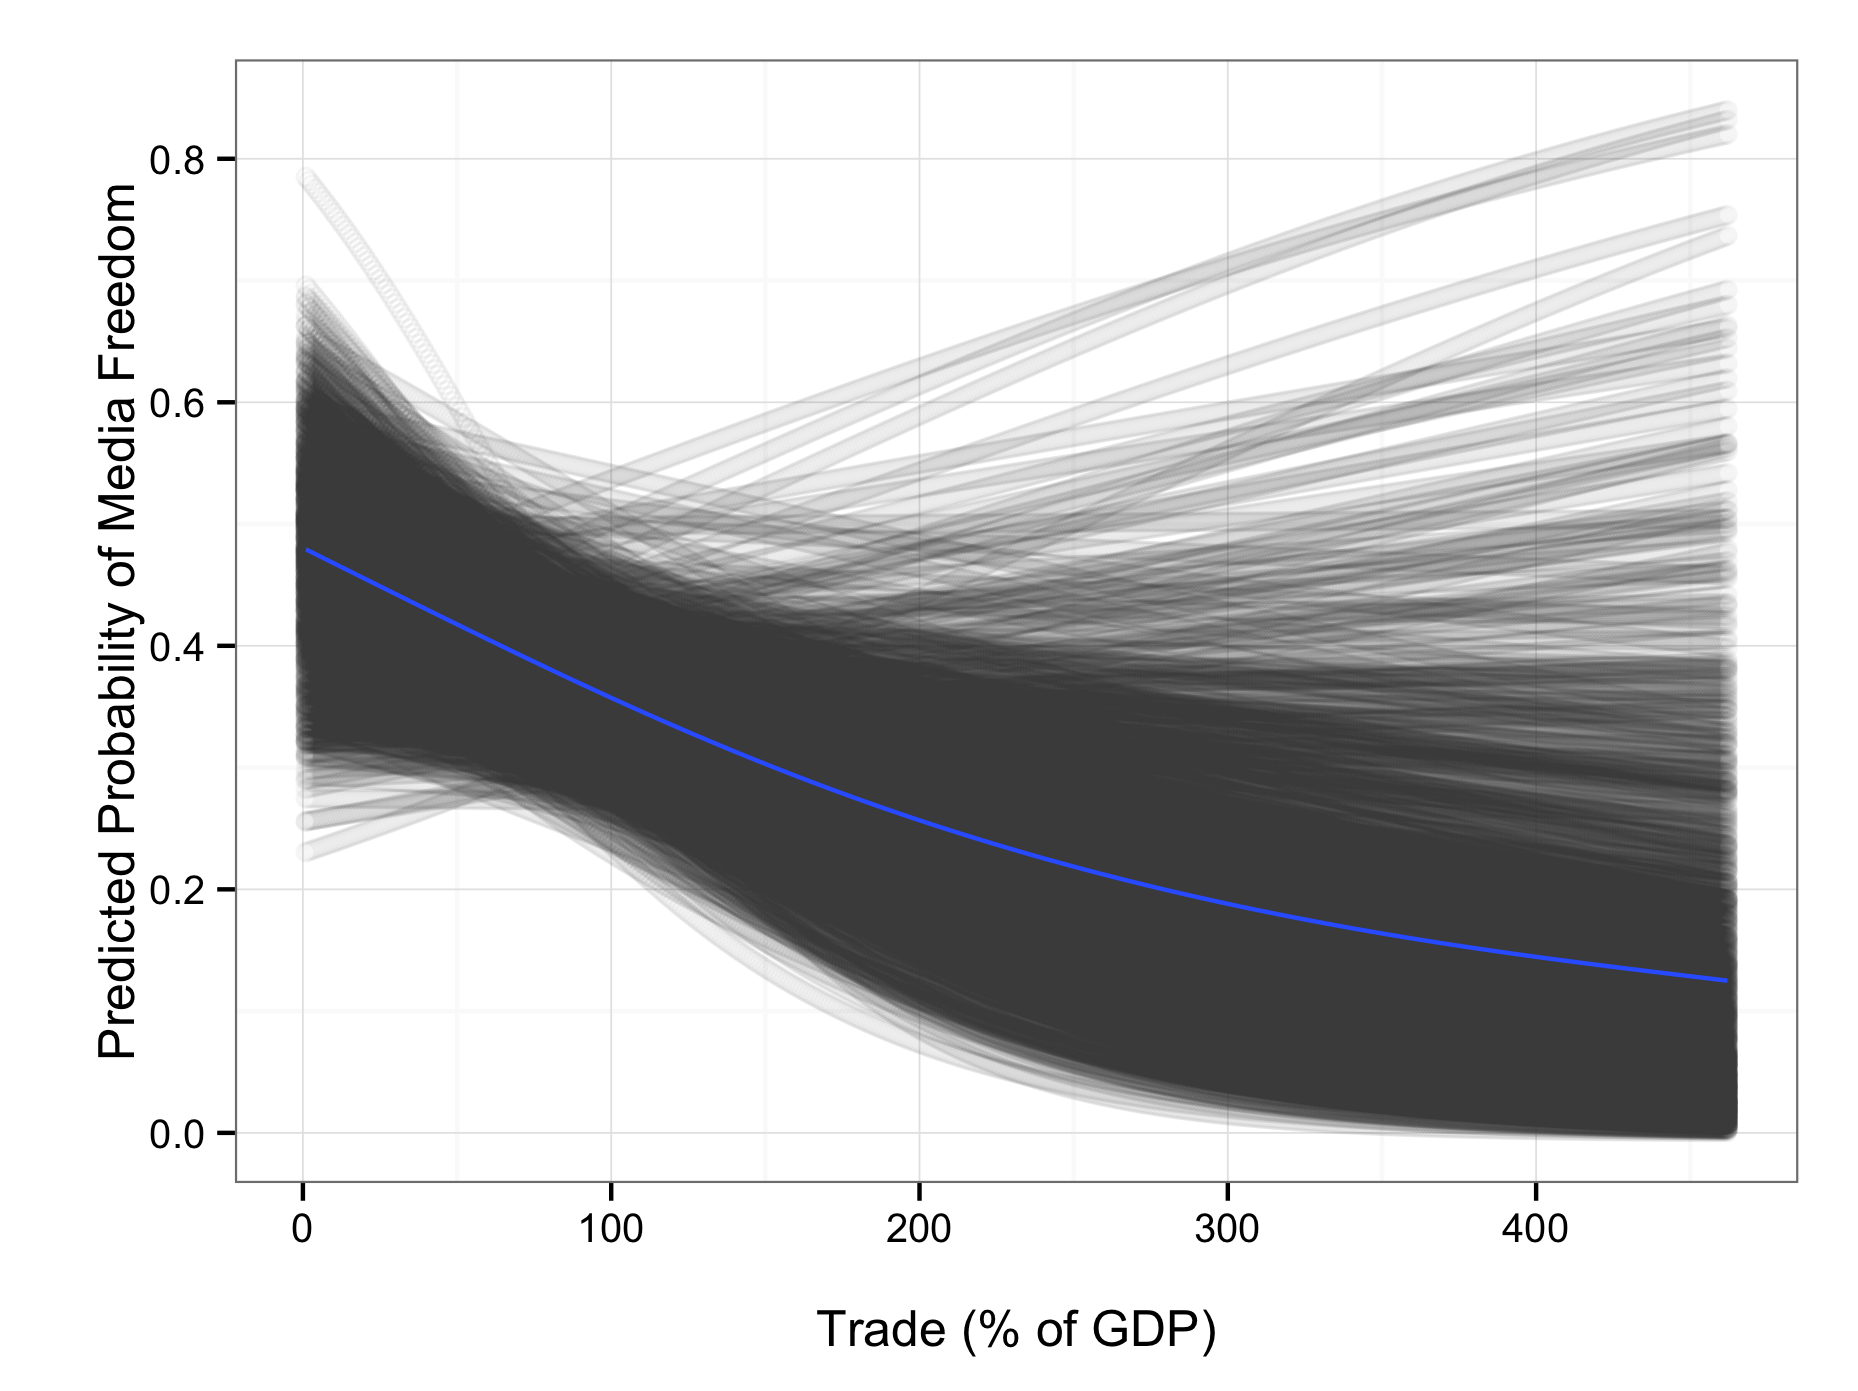
\includegraphics[scale=0.2]{article2_trade_effect_plot.png}
\caption{Predicted effect of trade on media freedom (1000 simulations with GAM smooth line)}
\end{figure}

\begin{figure}
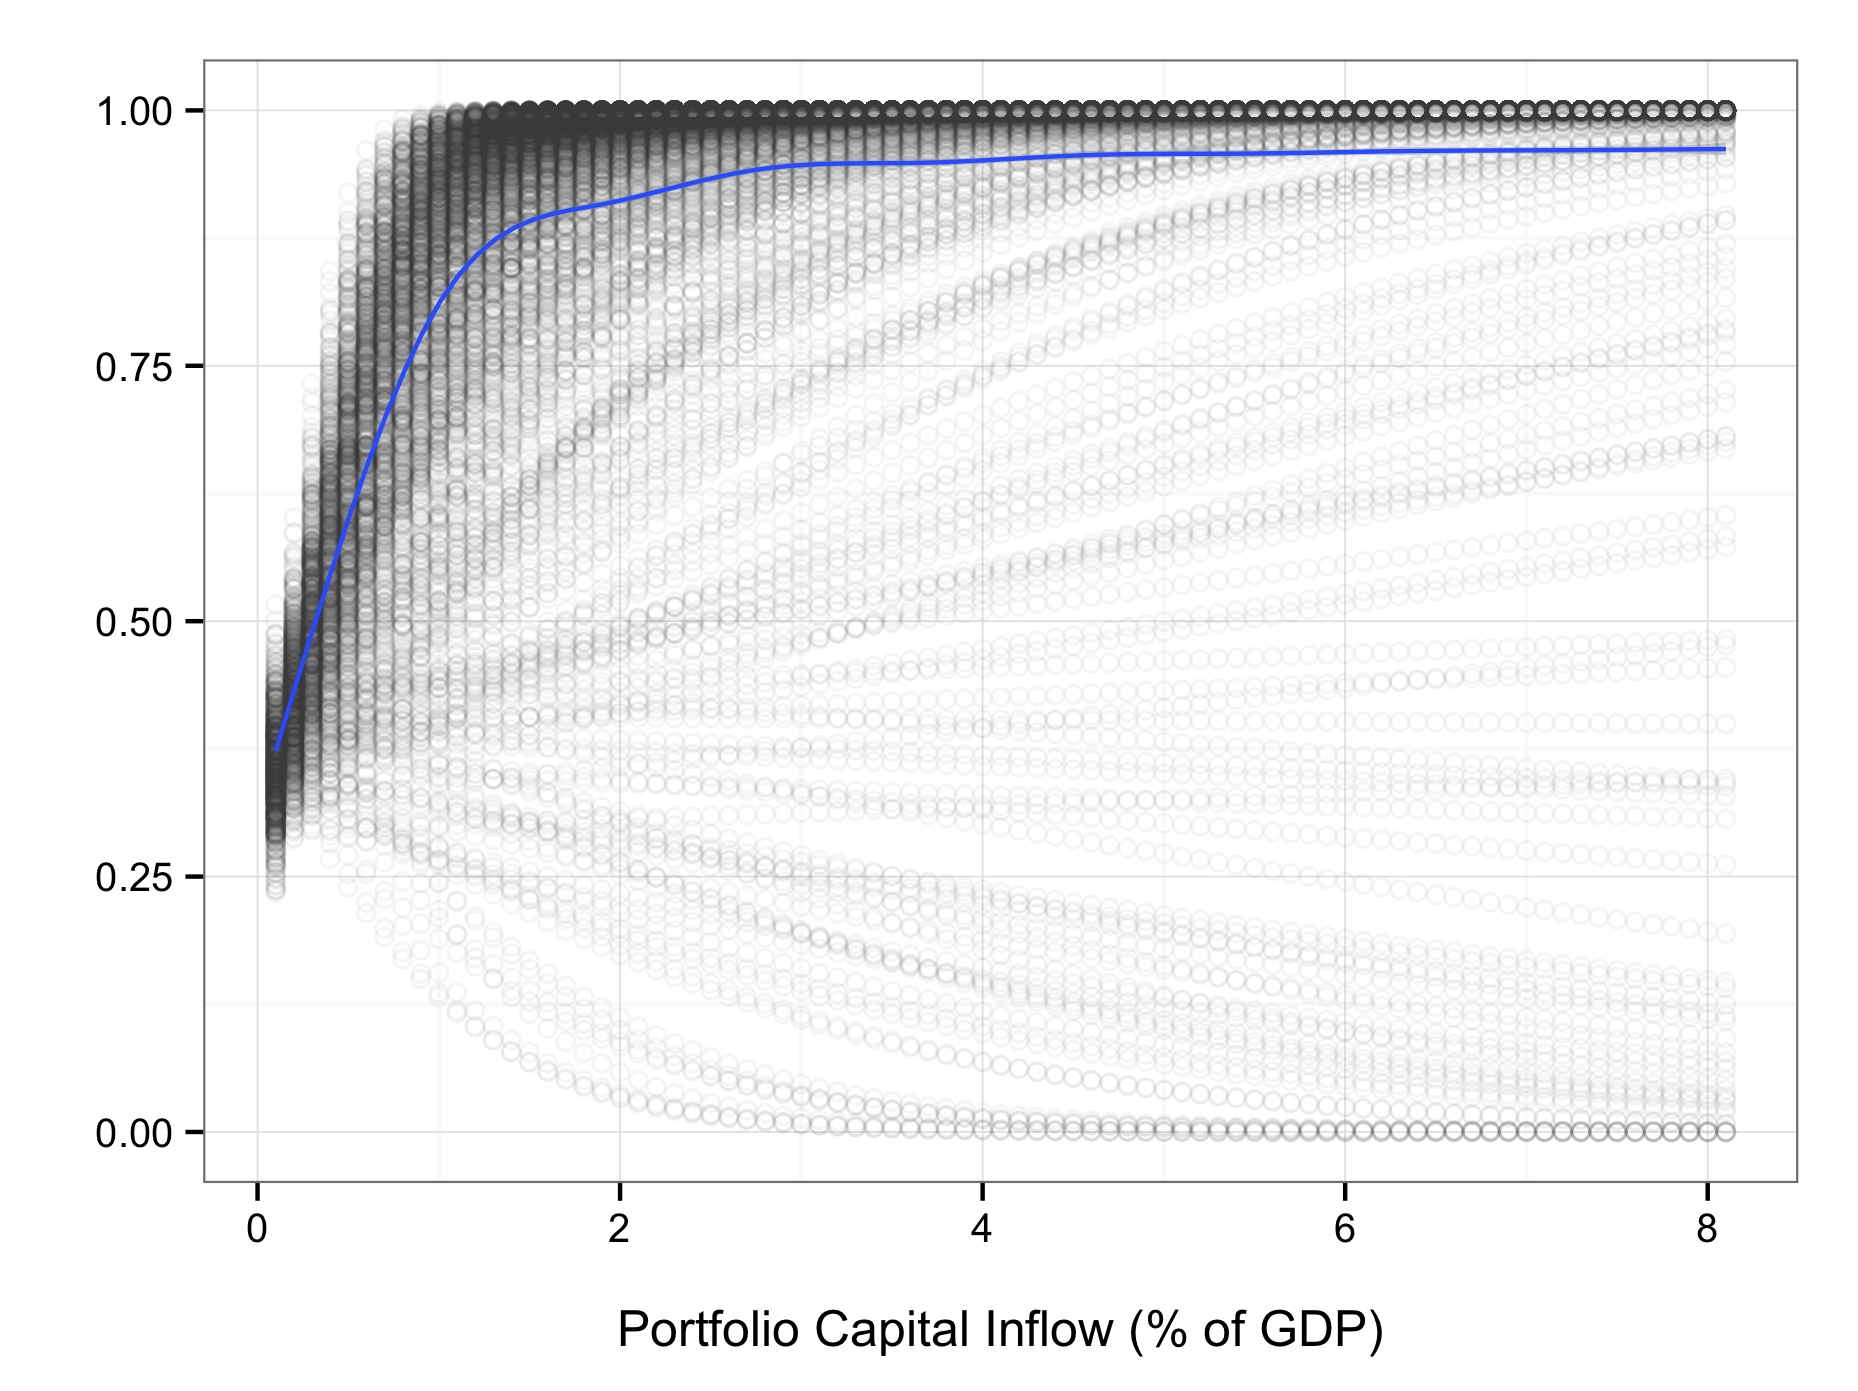
\includegraphics[scale=0.2]{article2_portfolio_effect_plot.png}
\caption{Predicted effect of inward portfolio capital level on media freedom (1000 simulations with
GAM smooth line)}
\end{figure}

\begin{figure}
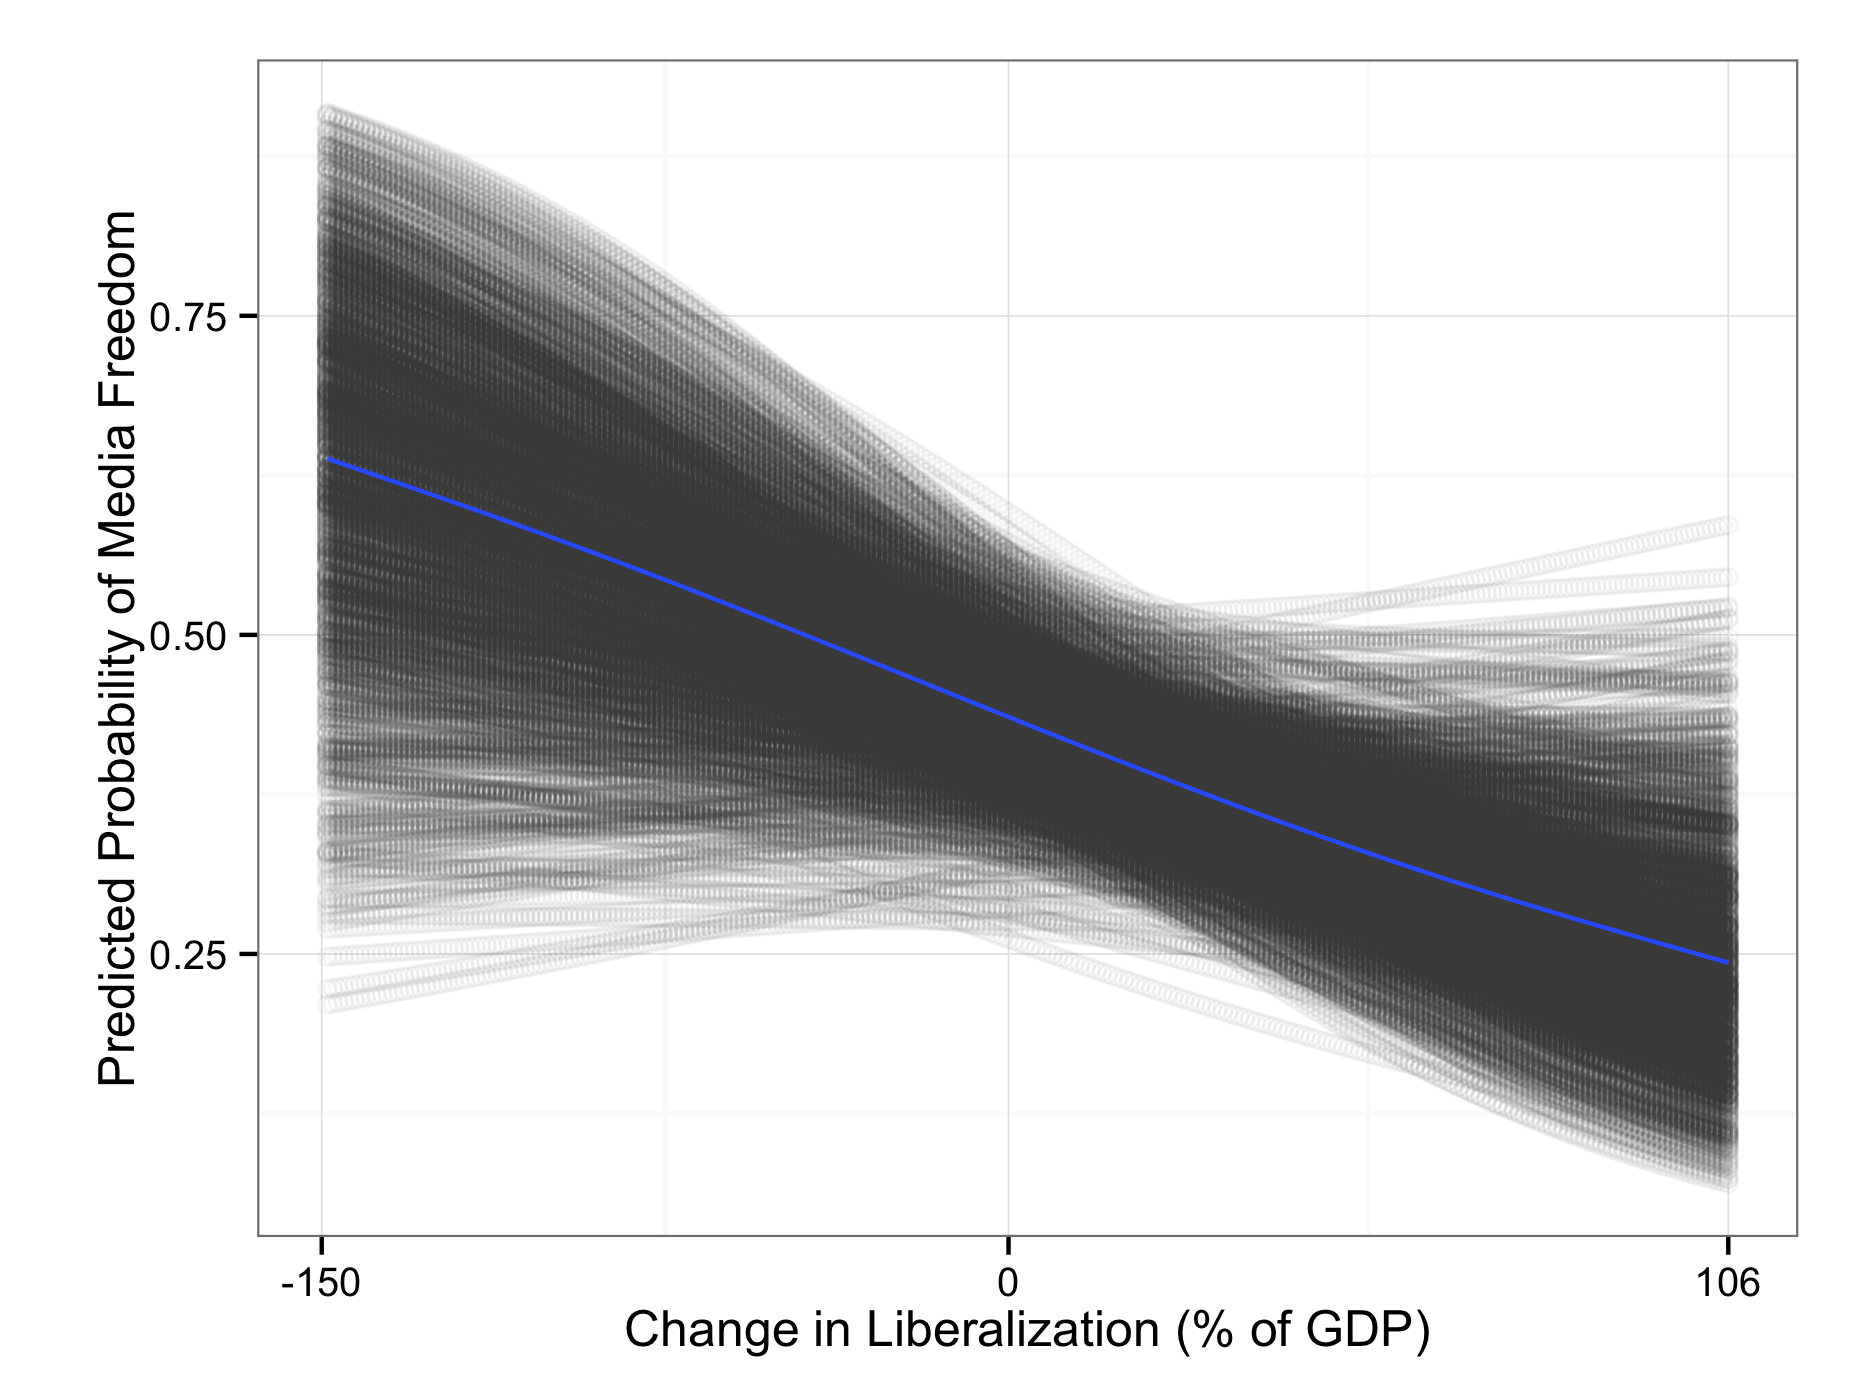
\includegraphics[scale=0.2]{article2_liberalization_effect_plot.png}
\caption{Predicted effect of year-to-year change in additive index of openness}
\end{figure}

\end{centering}

\subsection{Checking Reverse Causality with Panel VAR}

If already repressed media environments are more likely to open their economy, then it is possible
that our interpretation of the data wrongly specifies the direction of the causal effect. To test
whether trade openness tends to precede media repression or media repression tends to precede trade
openness, I use a method of vectorautoregression for panel data. Here I use only the continuous
numerical measure of media freedom supplied by Freedom House, beginning in 1994. The panel vector-
autoregressions suggests that shocks to trade affect press freedom, controlling for democracy and
GDP per capita, although the effects decay quickly. There is no evidence that press freedom affects
trade.

\begin{centering}
\begin{figure}
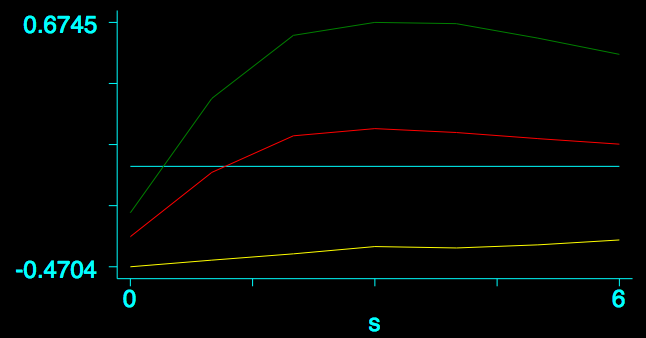
\includegraphics[scale=0.5]{article2_var_trade.png}
\caption{Impulse response of press freedom to a one standard deviation shock to trade level at t-2,
with democracy and GDP per capita endogenous; Green and yellow lines represent 95\% confidence
intervals drawn using Monte Carlo simulation (500 repetitions)}
\end{figure}
\end{centering}

\subsection{Within-Case Analysis}

In this section, I turn to the brief case studies of Argentina and Mexico to assess qualitatively
whether we can observe implications of trade liberalization generating pressures toward media
repression.

\begin{centering}

\begin{figure}
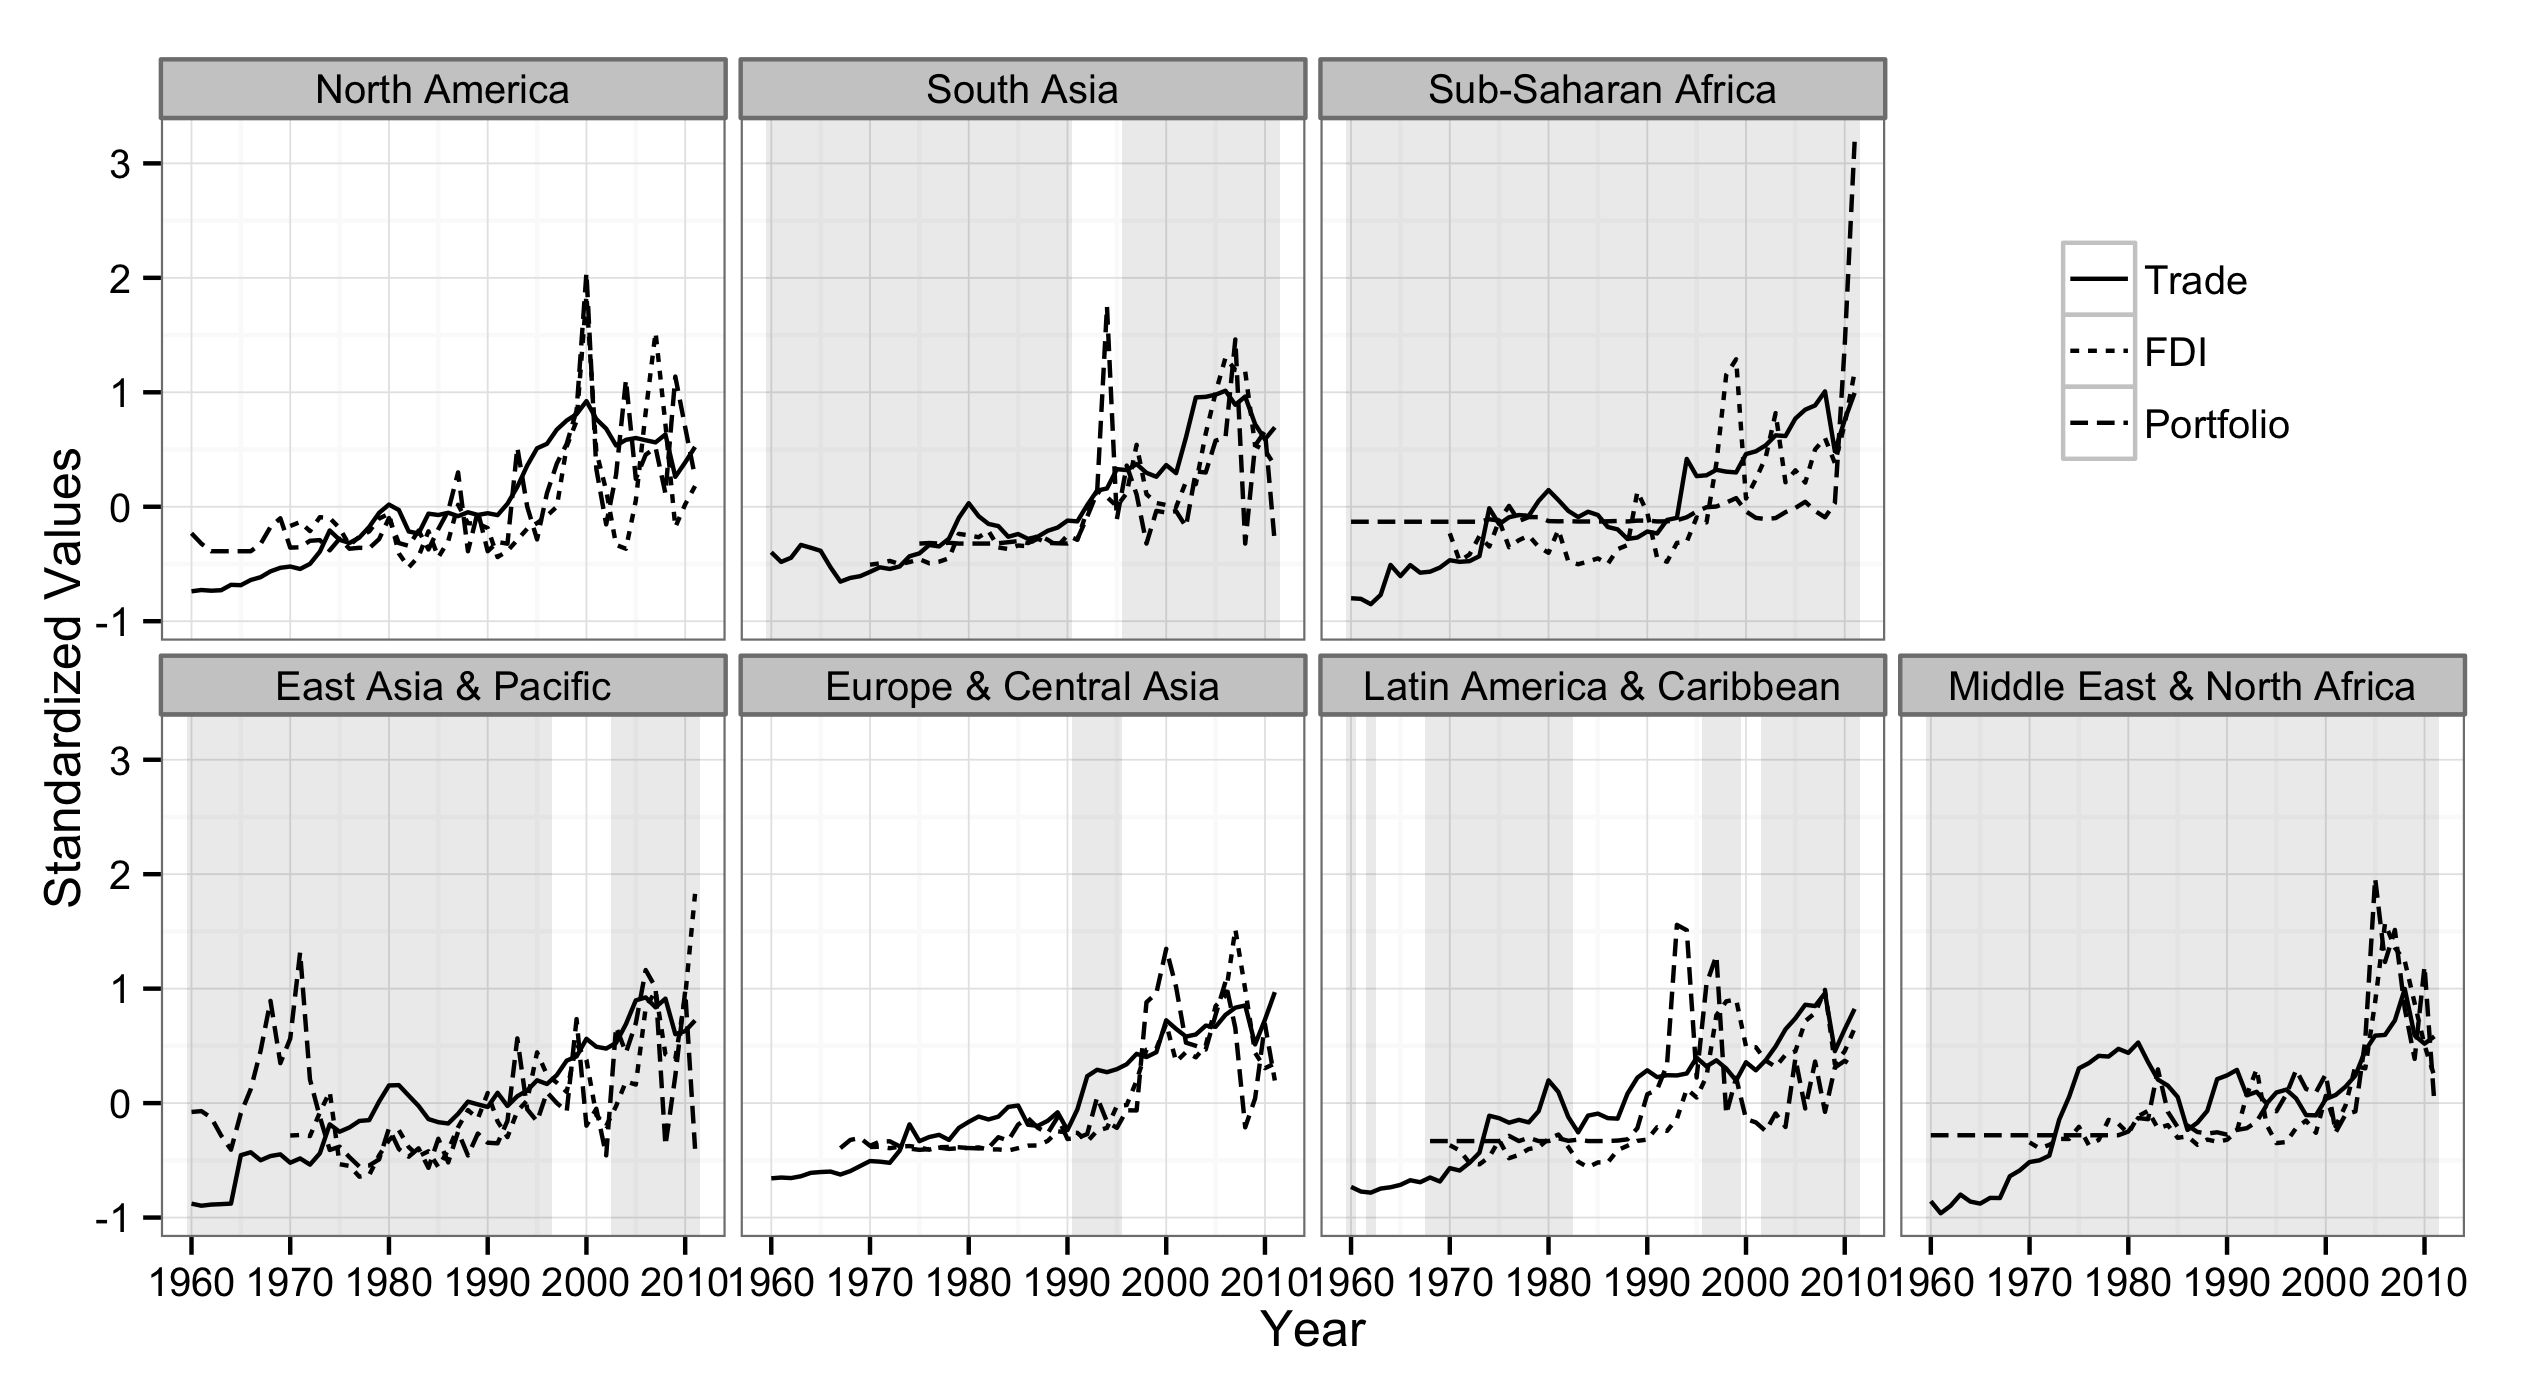
\includegraphics[scale=0.2]{article2_regions.png}
\caption{Economic Openness and Press Freedom 1960-2011, By Region}
\end{figure}

\begin{figure}
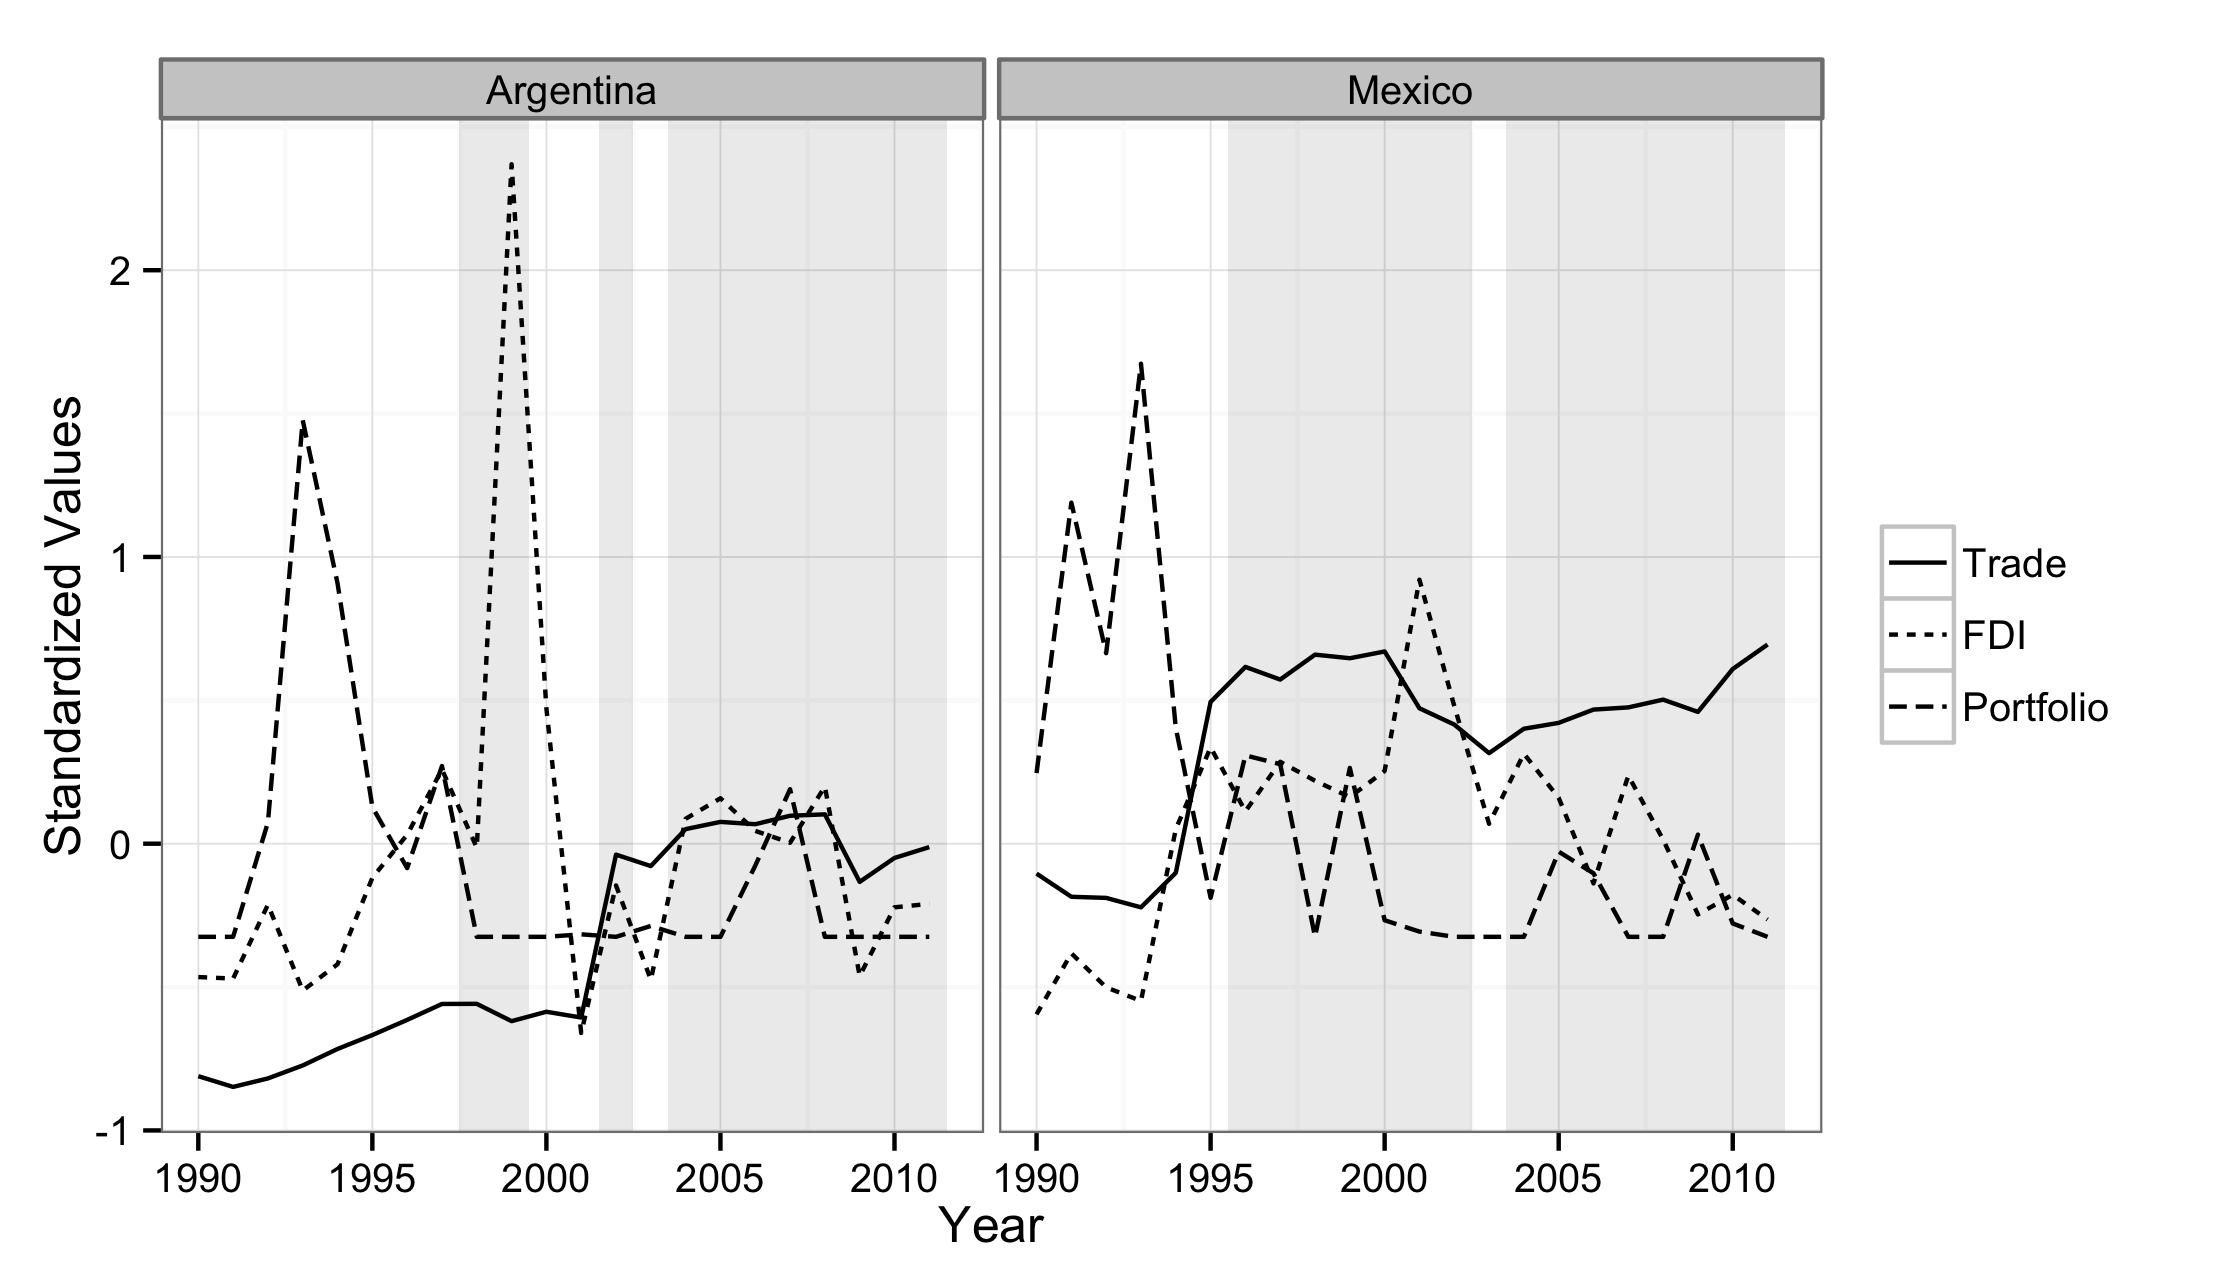
\includegraphics[scale=0.2]{article2_AM_cases.png}
\caption{Levels of openness and press freedom in four countries, 1990-2011 (standardized within countries)}
\end{figure}

\end{centering}

\subsection{Argentina}

Immediately upon inauguration as President in 1989, Carlos Menem announced a package of neoliberal
economic reforms which include liberalization of international trade and capital flows, as well as
privatizations and spending cuts. (\citealt[189]{Tommasi:1995wx}; \citealt{Borner:2002cp}). In the
beginning of 1989, the average tariff rate is 39\% (a maximum import tariff was 50\% with a tariff
surcharge of 15\% on all imports). By the end of 1989, the maximum tariff is 35\% and the average
tariff rate falls to 12\%. In 1990, all import licensing requirements are abolished and tariffs are
reduced across-the-board to 21\%. By 1995, the average unweighted tariff is 10.5\% and non-tariff
barriers as well as export restrictions are removed (\citealt[7]{Beker:2011vq}).
\footnote{Exemptions were made for IT, domestic appliances, and autos. As a result, imports
increased from \$4.1 billion in 1990 to \$21.6 billion in 1994, while exports increased from \$3.7
billion to \$20.1 billion at the same time. See \citet{Beker:2011vq}.}

As import competition put pressure on previously protected firms, about 30\% of manufacturing
employment was destroyed between 1992 and 1996. In those industries where import penetration
increased the most, wage inequality also widened during this period. Argentina's Gini coefficient
for income inequality, one of the lowest in Latin America at the time, increased from 40.0 in 1991
to 47.4 by 1998. (\citealt[505]{Galiani:2003fr}; \citealt[11]{Beker:2011vq})

Argentina will join the Mercosur customs union in 1991 and sign a trade agreement with the United
States in 1994. The reform package largely succeeded in taming inflation rates and growing the
economy. The inflation rate shrinks from 5\% in 1989 to .16\% by 1996 and gross domestic product
grows by 40\% between 1990 and 1994 (\citealt[4]{Beker:2011vq}). The IMF, World Bank, and the US
government saw Argentina as a model student in this period (\citealt{Cavallo:2004ta}:
\citealt[142]{Cavallo:2004bf};\citealt{Klein:2002vg}) and is frequently cited in leading
international publications such as The New York times and Time Magazine as a poster child for how
neoliberal economic reforms can be implemented democratically (\citealt{Anonymous:VVaTefru}as cited
by \citealt{stokes2001public};\citealt{Silverstein:2002wm}).

Although the reform package succeeds in taming Argentina's hyperinflation and creating economic
growth, the most immediate and direct effect of trade liberalization was an increase in
unemployment, especially among the workforce employed in previously protected, labor-intensive
industries (\citealt[10]{Beker:2011vq}). Additionally, trade liberalization reduced the income of
small-scale producers who could not compete with cheap imports (\citealt{eckstein2001power}).
Although trade liberalization is costly to the sizable constituencies of unskilled industrial
workers and rural campesinos, the government provides little public support for dislocated workers--
reducing rather than increasing public spending--until the government develops a targeted income-
assistance program during the currency crisis of 2001. This lack of government responsiveness
between 1990 and 2001 is puzzling given the longstanding expectation that governments, and
especially democratic regimes, must compensate domestic losers from liberalization in order to
sustain a sufficient political coalition in favor of liberalization. This expectation should be
especially strong for democratic governments, yet, despite the absence of government compensation,
Argentina sees relatively little domestic conflict around trade liberalization. In fact, there are
fewer strikes, strikers, and days lost to strikes than under Alfonsin (\citealt{eckstein2001power}).
Yet, dissent against liberalization was an observable current in public discourse in the years
before Menem's repressive media regulations.\footnote{It is worth noting that some of the media
scandals related to government corruption were themselves linked to international economic openness.
For instance, the aggressive Argentine daily Pagina/12, whose journalists were frequent targets of
violence, sparked a scandal when they reported on the Menem administration requiring ``substantial
payment'' from the meatpacking firm Swift-Armour before they were allowed to import machinery into
the country. Another highly publicized revelation involved the complicity of government officials in
an international drug-laundering network (Waisbord 1994).} Most notably in road blockages
organized by protesting farmers in 1991 and 1993, unfair international competition was a recurring
point of dissent. (\citealt{McCullough:1991cs}; \citealt{Ferber:1993fb}).

If the Menem regime neglected to make provisions for its harmed constituencies, how was it able to
enact and sustain dramatic trade and capital liberalization in a formally democratic setting? The
theory presented here expects that the Menem government is likely to repress the media in order to
silence domestic opposition to liberalization while maintaining a formally democratic front.
Consistent with the theory, the quantitative data reveal that after a long and stable period of
stable economic openness and media freedom under Alfonsin, media freedom is volatile immediately
after Menem's liberalization begins until it is stably repressed by 2005. According to a report
\emph{Agresiones a }La Prensa\emph{ 1991-1994} published by the Asociacion Madres de Plaza de Mayo,
around 452 acts of aggression were committed against the press between 1991 and 1994
(\citealt{Delgado:1995tr}, as cited in \citealt[247]{Park:2002io}). \footnote{Acts of aggression
refer to ``murder, death threats, bombings, bomb threats, intimidation, physical violence, violent
threats, and termination of broadcasts.'' If one were to count acts of excluding media from access
to the government and public name-calling of the media by the government, the figure would be 546.
} Although not perpetrated directly by the state, during this period there were many acts of
violence against investigative journalists critical of the Menem regime, acts which the government
denounced but treated with impunity. (\citealt{Long:1993wb}). The Menem family's most direct actions
against media freedom were cuts to state advertising in Pagina/12 (\citealt[27]{Waisbord:1994kq}),
11 lawsuits against journalists under the pretense of criminal defamation
(\citealt{McCullough:1991cs}; \citealt{Anonymous:TKNgfiRX}), proposals to increase libel and
defamation sentencing, and a proposal to require media outlets to purchase prohibitively expensive
libel insurance (\citealt{Sims:kgMPqAHd}).

\subsubsection{Mexico}

As in the case of Argentina, Mexico's trade liberalization in the 1990s was part of a larger
national project of neoliberal economic reform. Well before signing the North American Free Trade
Agreement (NAFTA) with the United States and Canada in 1994, Mexico unilaterally lowered tarrifs
from an average of 25\% in 1985 to 13\% by 1993 (\citealt{McDaniel:2003kw}).

Concurrent with unilateral trade liberalization and NAFTA, and as in the case of Argentina under
Menem, the Mexican government also privatized many state-owned enterprises and eliminated many state
subsidies and price controls originally intended to support small farmers. Most subsidies for corn
and wheat producers and retail food price controls were eliminatd by 1991
(\citealt[295]{Hufbauer:2005vh}). In 1999, the Mexican government abolished CONASUPO, the state
agency which bought staple crops at guaranteed prices and redistributed them to consumers
(\citealt[12]{Villareal:2010vk}).

After NAFTA, US imports from the US increased from \$50.8 in 1994 to 100.4 billion in 2000
(\citealt[10]{Villareal:2010vk}). As in the case of Argentina, trade liberalization through the
1990s hurt small farmers and non-skilled manufacturing, as agricultural employment decreased from
8.1 million in 1993 to 6.8 million jobs in 2003, and value added decreased from \$32 billion to
about \$25 billion in the same period.
(\citealt[289]{Hufbauer:2005vh};\citealt[14]{Villareal:2010vk}).

Also as in Argentina, increasing trade liberalization in Mexico led to increased wage inequality
between skilled and non-skilled labor. In 1988, the real average wage level of skilled Mexican
workers in the manufacturing sector was 225\% that of non-skilled workers. In 1996, it was about
290\% that of non-skilled workers, stabilizing until 2000 (\citealt[9]{Villareal:2010vk})

To support the transition into NAFTA, the government enacted the Programa de Apoyos Directos para el
Campo (Program of Direct Support for the Countryside or ``Procampo''), which provided farmers with
direct, hectare-based income support. However, in part due to austerity following the peso crisis,
total expenditure on Procampo decreased from \$1.4 billion to \$1 billion
(\citealt[295]{Hufbauer:2005vh}), despite the price of corn in Mexico falling from \$4.84 per bushel
in 1993 to \$3.65 in 1997 (\citealt[12]{Villareal:2010vk}), total number of supported farmers
decreased from 3.29 million to 2.95 million, between 1994 and 1998 (\citealt[295]{Hufbauer:2005vh}).

On the day NAFTA went into effect in January 1994, the Ejército Zapatista de Liberación Nacional
(EZLN) launched an armed uprising in one of Chiapas, one of Mexico's southernmost states. On that
very first day of the uprising, EZLN spokesperson Subcomandante Marcos declared NAFTA to be
``nothing more than a death sentence to the indigenous ethnicities of Mexico'' and their uprising to
be understood as a response ``to the decree of death that the Free Trade Agreement gives them''
(\emph{La Journada }1994, as cited in \citealt[216]{Hayden:2009uy}).

Although Procampo helped gain support for NAFTA, immediately there was popular discontent, such as
in the Barzón Farmers movement in Zacatecas, regarding several inadequacies of the program,
including payments not being made (\citealt[173]{Williams:2001ux}). From 1993 to 1995, Barzon
movement sought and received much favorable attention in the print media, where reporters were not
under great pressure to suppress reports (\citealt[187]{Williams:2001ux}).

Neoliberal economic reforms, including increasing trade openness, somewhat surprinsingly in light of
our expectations although not exactly contradicting them, led to a relative opening of the domestic
media (\citealt{lawson2002building}). Between 1991 and 1993, in addition to pursuing NAFTA as his
administration's top priority, Salinas' cuts to government spending included cutting the \emph{quid
pro quo's }which underwrote the traditional regime of media control. He specifically ended the
system of paying for reporters accomodations on presidential trips, prohibited the distribute of
bribes within the presidential palace, reduced the government advertising in which typically
functioned as bribes for keeping media in line, ended tax deferments and credits to media, and
stopped allowing media outlets to pay their Social Security taxes in advertisements. Privatization
of state-owned enterprises also had the effect of reducing the media's dependence on government
advertising revenues. The greater scrutiny from American and Canadian media relaxed the domestic
media environment for domestic journalists, as it was easier for domestic journalists to report on
topics that the foreign press were already reporting on outside any control from the Mexican
government. Additionally, greater access to foreign inputs also freed the Mexican media from an
important source of government leverage, in particular its traditional monopoly on the import of
newsprint, providing further room for the Mexican media to take risks. As independent media outlets
were gaining financial independence through market competition, at the same time the neoliberal
state was relinquishing its traditional levers of control, led to a independence of the Mexican
media increased significantly (\citealt[76, 89]{lawson2002building}).

The international spotlight from the NAFTA negotiations also forced Salinas to cultivate a more
positive image on human rights, for instance, when he established the National Commission for Human
Rights (\citealt[107]{Dominguez:2009wd}). Additionally, because neoliberal economic reforms actually
led to an opening of the media which the state could not control, Salinas and after him Ernesto
Zedillo moved away from traditional tactics of media repression in favor of more modern techniques
of ``news management'' and public relations, such as controlling information by only providing
access to friendly reporters. For instance, in a 1990 press conference Salinas explicitly excluded
several independent media outlets and only permitted the most reliable pro-government journalists.
Later in 1996, the Interior Ministry for the first time created an explicit ``blacklist'' of
journalists who government officials were supposed to not engage (\citealt[39]{lawson2002building}).

Newspaper circulation is limited in Mexico, whereas television broadcasting dominated by Televisa is
the main source of information, so it was dominated by pro-NAFTA, pro-government ideology
(\citealt{Hellman:1993wa}). They also used it for extensive foreign media campaigning. While
building support for NAFTA, Salinas used media and PR tools extensively, including efforts to
persuade Mexican-Americans and US investors to support NAFTA in the United States
(\citealt{Morris:2001iy}). This was the first time the Mexican government used advertising and
lobbying in its foreign relations (\citealt{Chabat:1997wj}) One of the most commented advertisements
urged US business to look to Mexico as a place where they can hire workers for a dollar an hour.
(\citealt[105]{center1993trading} as cited in \citealt[45]{Chabat:1997wj}).

This narrative reveals dynamics which are unexpected and in a crucial sense antithetical to our
theory, for they reveal how economic liberalization may induce greater media freedom by increasing
competition and growth. Yet, Salinas in particular was convinced that he had to protect the
government's image to succeed in his foreign economic policies (\citealt[107]{Dominguez:2009wd}).
Although economic reforms made certain kinds of repression impracticable, under Salinas and then
Zedillo the Mexican government engaged in specific acts to exclude the press from reporting on
politically sensitive issues. Lawson observes plainly that Salinas was historically Mexico's
``undisputed master of image management'' (\citealt[39]{lawson2002building}). Additionally, the
editor of Mexico's \emph{Monitor, }José Gutiérrez-Vivó, affirmed in 1996 that ``Salinas was the
president who was hardest on the media. He was the one who sought the most control over the
media.''(\citealt[39]{lawson2002building}) After NAFTA passes, intimidation and direct violence
against journalists at the hands of the state can still be observed, as when the state expropriates
the property of critical editors (\citealt{OrmeJr:1997da}). In fact, despite a de facto opening of
the media due to financial independence and the neoliberal withdrawal of the state from private
enterprise, federal state-media relations changed little until Zedillo and even his adminstration
engaged in repressive tactics such as arresting the publisher of \emph{El Universal} for tax-related
reasons in 1996. Finally, physical assault against journalists increased throughout the period of
Mexican media's opening from 1980 to the middle of the 1990s (\citealt[81]{lawson2002building}),
which was also a period of dramatic trade opening. Most of the physical assaults were not carried
out by the government, but they were largely treated with impunity by the government, such as in
1996, when two journalists were murdered more ``savagely'' than ever before in Mexico.
(\citealt{Anonymous:ex})

\subsection{Summary of cases}

Thus, in the process of trade liberalization, Mexican state officials actively seek greater control
over the media as much as they can, despite the effect of increased competition unleashing an
increasingly independent media. Both Salinas and Zedillo employed a variety of tactics ranging from
traditional repression to modern ``news management'' in order to control their image in the media
during a period of rapid trade liberalization. Salinas in particular, the earliest and most
aggressive proponent of economic liberalization in the late 1980s and early 1990s, tried more than
anyone else to control the media.


\section{Conclusion}

I find broad support for the hypothesis that trade openness is negatively associated with media
freedom because, whereas international investors of FDI and portfolio capital prefer media freedom
to media repression in the long run, the international counterparties to foreign trade have no such
preference. Thus, although all three types of economic openness are associated with media repression
in the short run, trade openness is associated with media repression in the short- and long-run.

The implications are important for researchers of the globalization-democracy nexus because they
highlight a specific way in which economic globalization can generate authoritarian tendencies. The
case studies reveal that even for the most celebrated neoliberal economic reformers of the 1990s,
Menem in Argentina and Salinas in Mexico, the opening of the domestic economy was followed by
government efforts to repress the media through a variety of tactics.

Certain unexpected findings also suggest interesting questions. For instance, when economic
liberalization increases market competition in the media sector, it generates strong pressures which
favor a free, independent media. If this is the case, then it would provide a warrant for expecting
trade liberalization to be associated with media freedom in the long run, as the conventional wisdom
is that trade liberalization increases market competition. Thus, if trade indeed is associated with
increased domestic competition, then it remains unclear why trade liberalization would be
statistically associated with media repression in the long-run, a pattern evidenced in the
statistical models here. One possibility is that the domestic economic and political consequences of
trade liberalization are not fully understood and that trade liberalization independently is not
associated with increased domestic competition.


%%%%%%%%%% CHAPTER BREAK %%%%%%%%%%%%%%%%%%%%%%%%%%%%%%%%%%%%%%%%%%%%%%%%%%%%%%%

\chapter{Mass Media and the Social Construction of Globalization}

A long tradition of scholarship going back to Karl Polanyi's \emph{The Great Transformation}
(\citeyear{Polanyi:2001vc}), suggests that when exposure to free trade increases, there typically
follows a corresponding increase in demand for economic and social support from the state. Scholars
of political science and economics have updated and extended this logic to show that exposure to the
global market is often positively associated with government spending (\citealt{Adsera:2002vt,
Cameron:1978vb, Garrett:1998wl,Rodrik:1998te}). However, in analysis presented here, survey data
shows that demand for public intervention in response to increasing exposure to the global market is
not universal; increased exposure to the global market is met, in some cases, with less demand for
public intervention. This is very puzzling, given the expectations implied in the globalization-
welfare argument.

	I argue that the solution to this puzzle is that individuals and groups do not perceive
	globalization in a simple, unmediated fashion. The media---a set of actors often neglected by
	IPE scholars---filter the experience of globalization. Furthermore, the owners of media outlets
	often have large stakes in how globalization is perceived within a country. Specifically, I
	hypothesize that when the state itself or foreign companies own media outlets, they will seek to
	represent globalization in a way that dissociates it from demands for public support. Foreign
	media companies will do so because their presence in the host country relies on domestic support
	for foreign investment and foreign ownership. State companies will do so to dampen public outcry
	and the demands for public support often associated with exposure to free trade.

	To demonstrate these claims, I provide evidence from three levels of analysis. I first use
	statistical analyses to relate conventional measures of global market exposure to attitudes
	regarding state intervention in the economy. My analysis uses data from the World Values Survey
	and covers 50 countries from 1991 to 2009. Secondly, I provide quantitative within-case
	evidence. A sudden transfer of media ownership in New Zealand during 2003, from mixed to
	strictly foreign ownership, provides an attractive opportunity to examine variation on the
	independent variable over time. Finally, I demonstrate that the effect of this shift in
	ownership can be traced at the textual level, providing qualitative evidence that the media
	representation of globalization is observably different before and after an increase in foreign
	ownership of the media company. In summary, my findings provide promising evidence---although
	somewhat mixed---that the degree to which globalization is met with a demand for public support
	is likely conditioned by the interests of the media owners responsible for constructing
	globalization; and that an observable change in reportage is the mechanism by which this
	conditioning effect is realized.

The paper proceeds in four parts. The first section provides a review of literature on the
globalization-welfare nexus and a review of literature on the effects of media ownership, focusing
on the untested assumptions of the former and unexplored connections between the two. The second
section offers a model of the globalization-media-welfare nexus and hypotheses regarding the
observable implications of the model. The third section explains the data, methodology and the
triangular research design. The fourth section presents the core statistical and qualitative
findings, and the fifth section concludes. Overall, the findings problematize critical assumptions
in the globalization-welfare literature and provide strong evidence---although somewhat mixed---that
the social construction of globalization impacts the political response to changes in global
exposure.

\section{Literature Review: Globalization, Welfare, and the Media}

Responding to the widely-held expectation that globalization implies the end of the welfare
state, scholars of international relations (IR) and comparative politics have argued that
exposure to global markets is positively and significantly associated with government spending
(\citealt{Cameron:1978vb, Ruggie:1982wx, Katzenstein:1985ub, Baek:2009vq, Rodrik:1998te, Garrett:1995tj, Garrett:1998wl, Adsera:2002vt}). The dominant theoretical explanation of this regularity is some form of a
``compensation" thesis, which suggests that in order to build a winning coalition in favor of
free trade, to legitimate openness, or to hedge against external risk, governments must
compensate with public support those who suffer from the opening of domestic markets. Although
scholars debate particular components of this general finding, and there is an increasing effort
to disentangle the specific effects of specific aspects of globalization (\citealt{Burgoon:2001dp}), there
is much empirical evidence in favor of a general claim that national governments often seek
compensatory domestic strategies in response to the changes and dislocations wrought by the
opening of domestic markets to global exposure.
	
Although there appears to be robust empirical evidence of the link between exposure to global
markets and government spending, there is much less empirical evidence of the micro-processes
supposed to explain this link. Specifically, most empirical studies of the globalization-welfare
nexus implictly or explicity make two assumptions: 1) Those individuals or groups likely to be
harmed by increased free trade know or believe that freer trade will cause them harm and 2) see
increased government spending as a desirable compensation (\citealt{Rodrik:1998te}, 998).

Very little research has sought to demonstrate either of these assumptions in particular,
despite that they involve attitudinal implications one should be able to observe in survey data.
Although there is a great deal of research on preferences toward free trade, there exists little
research on how preferences toward domestic politics are shaped by free trade. Hays, Ehrlich,
and Peinhardt (\citeyear{Hays:2005vo}) observe that the micro-processes underwriting the empirics of the
globalization-welfare nexus have been neglected, but their own study only tests whether social
spending is, in fact, associated with support for free trade. It remains an open question
whether, or under what conditions, mass attitudes in fact reflect an interpretation of
globalization as necessitating a governmental response.

Although empirical research on the attitudinal assumptions of the compensation thesis has been
largely neglected, recent research suggests that government spending as a response to global
exposure is significantly conditioned by domestic political factors more generally. For
instance, Adser\`{a} and Boix show that authoritarianism is an alternative to compensation: the
government may simply exclude from any consideration those who suffer from exposure to global
markets (2002). Because of this, the relationship between globalization and increased spending
is not as strong under authoritarian regimes. This suggests that the state is a strategic actor
that will seek an alternative to the compensation strategy under certain conditions.

Students of American politics regularly study the mass media as a political institution
(Hollifield 1999) having significant effects on attitudes and political behavior (Weaver 1996;
Newton 1999; Druckman and Parkin 2005). Yet, for the most part, there is very little research on
the relationship between the international political economy and the media. Although there
exists an abiding scholarly interest in ideational notions such as social purpose and the
determinants of its construction (Moravcsik 1998; Abdelal 2001; Abdelal, Blyth, Parsons 2010),
only isolated qualitative research has raised the question of mass media's involvement in
constructing aspects of the global political economy (Sklair 1997; Prakash 2002; Clark, Thrift,
Tickell 2004). Given the growing success of institutionalist scholars seeking to understand how
domestic institutions affect the aggregation of domestic interests and policy outcomes at the
international level, it is suprising that the mass media have been neglected from an
institutionalist perspective.

Yet, extant research gives good reason to expect that media ownership in particular will have
significant effects on attitudinal (and, in turn, governmental) responses to globalization.
First, some Americanists find that editorial bias does indeed affect vote choice (Druckman and
Parkin 2005). Second, scattered research on newspaper journalism has shown evidence that the
business interests of owners are related to the direction of editorial slant. For instance, an
early study by Pratt and Whiting (1986) studied editorials concerned with broadcast deregulation
between 1983 and 1985 and found that newspapers owning or owned by broadcast interests were
significantly more likely to editorialize in favor of broadcast deregulation. Furthermore, Ann
Hollified (1999) finds that foreign ownership of newspapers is positively associated with
editorials about events emanating from the country of the owner(s). If the political logic
underwriting the compensation thesis is that politicians have to compensate those who lose from
globalization in order to protect their electoral prospects, then the twin findings that
editorial slant affects vote choice and that the interests of media owners shape media bias
represent compelling \emph{prima facie} evidence that the owners of mass media play an important
role in the globalization-welfare nexus.

In sum, although exposure to the global market is often found to be positively associated with
government spending, it remains an open empirical question whether the response of mass publics
toward such exposure is, in fact, the demand or even desire for government compensation.
Furthermore, although research in IPE and comparative politics suggests that domestic
institutions mediate this response, the effects of the mass media have not yet been studied in
this context, despite strong empirical and theoretical reasons for doing so.

\section{A Theory of Media Ownership and the Social Construction of Globalization}

Despite the implicit assumptions of most empirical research on the globalization-welfare nexus,
globalization is not a self-evident phenomena. Strictly speaking, no citizen of any country ever
experiences globalization. Rather, citizens experience the effects of fairly complex economic
processes rarely, if ever, observed. To the degree that exposure to international market forces
takes the shape of something for which government leaders have to compensate their
constituencies, such international forces have to be identified and explained to those who would
suffer from them. Knowledge of and opinions regarding the effects of globalization may be
determined by heuristics and cues from professional associations, trade unions, and government
leaders. But arguably it is the owners and journalists of the mass media that are the most
powerful set of actors charged with identifying and explaining political forces not directly
observed by the public. Because the interests and incentives of media owners are not necessarily
consistent with the mass publics they serve, I argue that the response of mass publics toward
the global economic exposure of their home country will vary according to the different
interests of different types of owners. The mechanism by which this causal connection is likely to be realized is variance in how globalization is represented in media reports. Different kinds of media owners are biased by different incentives and are therefore likely to represent globalization in observably different ways, ways which are marginally more likely to produce mass attitudes consistent with the owners' interests. If the standard model of the
globalization-welfare literature is

\begin{center}
$globalization \rightarrow domestic$ $policy$ $response$
\end{center}

then the model presented here argues and tests whether media ownership intervenes in this causal chain:

\begin{center}
$globalization \rightarrow media$ $ownership \rightarrow reportage \rightarrow
attitudes \rightarrow$ $policy$ $response$
\end{center}

Local, non-publicly-owned media companies (LNPCs) have an interest in reporting the local costs of
internationalized domestic markets. Insofar as foreign media conglomerates are better resourced,
competitive rivals to LNPCs only to the degree that the domestic media market is open to foreign
ownership, LNPCs have a direct interest in constructing globalization as a problem. If public
sentiment toward globalization might impinge on domestic political decisions to open domestic
markets, the bias of LNPCs will lean toward a construction of globalization more likely to engender
protectionist sentiments than pro-free-trade attitudes. A public overly enthusiastic about opening
domestic markets could be the sufficient condition for a government to permit the domination of
LNPCS by foreign-owned conglomerates.

Local, publicly-owned media companies (LPCs) have strong incentives to construct globalization as
relatively innocuous, or at least to blur the direct causal connection between the opening of
domestic markets and the adjustment costs faced by actors in the local economy. If the compensation
thesis is at all correct, then governments must be cognizant that there are direct political costs
to opening domestic markets. But compensating those who lose from free trade with increased public
support is only one solution, and evidently a costly one. It follows from the logic of the
compensation thesis that blurring the public understanding of the causal link between free trade and
its adjustment costs lessens the political necessity to provide compensation. In short, a government
will not be held responsible for providing compensation if the public does not blame its woes on
particular government decisions to internationalize domestic markets. Thus, media companies owned by
the government have an incentive to construct globalization in a way that dissociates
internationalization from its costs.

Foreign-owned media companies (FCs) have interests opposite to those of LNPCs but aligned with LPCs.
Because the very right to operate and earn profits in a host country requires positive and
potentially reversible political action from the host government (through often controversial legal
reform on precisely this issue), foreign-owned media companies have direct stakes in public
sentiment toward an open domestic market in the host country. Should accurate knowledge of the costs
of globalization around the world make the public weary of foreign investment in their own country,
foreign-owned media companies could very well lose access to that market altogether. This implies a
powerful incentive for foreign-owned media companies to construct the phenomena of globalization as
relatively innocuous.

Predicting \emph{a priori} how bias toward globalization will manifest itself at the level of media
representations is difficult. If state or foreign ownership biases media in favor of globalization,
this could manifest itself as over-reportage of the benefits of globalization or an under-reportage
of globalization as a contestable and controversial political development. Thus, rather than
theorize about sheer volume of reportage under different ownership structures, we may theorize about
the functional relationship between globalization and its reportage. That is, we would expect a
perfectly unbiased media outlet to simply mirror the world, in which case there is likely to be a
strong functional relationship between processes of globalization and reportage of globalization. A
media outlet biased in favor of globalization may either over-report globalization positively or
under-report globalization negatively, but apart from volume we would also expect to see reportage
patterns functionally disconnected from real-world events. In short, bias would imply a reporting
agenda (whether positively or negatively) out of sync with the fluctuation of real-world events.

\subsection{Hypotheses}

From the state of extant literature on the globalization-welfare nexus, and
from the theoretical argument developed here, several hypotheses can be elucidated.

\singlespacing \begin{quote} H1. Other things equal, a country's increased exposure to the global
market will be positively associated with preferences for compensatory government intervention.
Phenomena of globalization such as foreign direct investment, importing and exporting, and financial
inflows and outflows should increase the preference of mass publics for the governmental moderation
of free-market consequences. This is implied in the compensation thesis. \end{quote} \doublespacing

\singlespacing \begin{quote} H2. In countries wherein foreign \emph{or} public ownership dominates
media markets, the causal link between globalizing processes and preference for government
intervention will be significantly less or possibly even reversed. That is, foreign or public
domination of media will interact with the phenomena of globalization to reduce the latter's
positive impact on preferences for government intervention. In extreme cases, foreign-public
oligopoly in media markets might condition the effect of globalizing processes so much that exposure
to global markets \emph{decreases} preferences toward government intervention. \end{quote}
\doublespacing

\singlespacing \begin{quote} H3. Media outlets owned by foreign or public companies are less likely
than LNPCs to report on globalization as a function of immediate national experience. Whereas LNPCs
have an interest in covering globalization precisely to the degree that globalizing processes
penetrate or threaten to further penetrate their country, FCs will cover globalization in a blanket
fashion disconnected from national experience. This hypothesis is agnostic with respect to the
quality or connotation of such reporting; its testable implication involves the functional
relationship between quantity of phenomena and quantity of reportage.\end{quote} \doublespacing

\singlespacing \begin{quote} H4. Because they have an interest in constructing participation in the
global economy as a contestable domestic policy choice, LNPCs are more likely to construct a
country's experience of globalization as the outcome of a contestable domestic political decision
with winners and losers, proponents and critics; state-foreign oligopolies are less likely to
construct globalization as a controversial decision, and more likely to construct it as an
ineluctable, objective process. In short, a qualitative analysis of media reports under different
ownerships should reveal a discernibly different representation of globalization, moving from what
we might term a contested change to a naturalized occurrence. This hypothesis is independent of
quantity or functional relationship and involves only a qualitative difference, at the level of
media representations. \end{quote} \doublespacing

The null hypotheses are that processes of globalization have no relationship or a negative effect on
attitudes toward government intervention; that media ownership does not significantly interact with
processes of globalization to affect attitudes toward government intervention; that the functional
relationship between globalization and reportage is not significantly different under the specified
ownership types; and that qualitative analysis is unable to identify any clear and distinct
difference in the tone or content of media reports under different ownership types.

\section{Data and Method}

Because the theory developed here makes theoretical claims about a two-staged process (media
representation and the response to it), and because for sampling reasons the quantitative data
presented is less than ideal, I provide three empirical angles to test the theory developed above.
Although these angles access the observable implications of the model at different stages and thus
test for the presence of distinct relationships, the conclusions from each angle reinforce each
other insofar as they represent the moving parts of one theoretical machine. For instance, if the
quantitative data is consistent with the theoretical expectation that state or foreign ownership
dampen the political backlash to free trade but the data preclude conclusive tests, qualitative
evidence that state- or foreign-owned media are biased in favor of globalization not only supports
the hypothesis of that process but also the dampening process. This is because the bias is a
constituent element in the dampening process. Thus, rather than attempt the unrealistic projects of
a perfectly conclusive set of statistical tests, or a soundly generalizable case study, this paper
opts for an ``analytical eclecticism (Sil and Katzenstein 2010)."

\subsection{Globalization and Preferences Cross-Nationally}
In the first half of the analysis, cross-sectional time-series regressions are presented on three measures of globalization and three measures of demand for state intervention, using data from 49 countries between 1990 and 2008. A list of countries is included as an appendix. All of the main economic data is from the World Bank
Indicators and lagged by one year.  The data on preferences come from the first four waves of the
World Values Survey. The data is less than ideal for all the model specifications one might like to
consider, so I estimate, as the data permit, a combination of models using ordinary least-squares
(OLS) with panel-corrected standard errors (PCSE) and generalized least-squares (GLS) models, with a
combination of corrections for autocorrelation. All estimated models use PCSE, the conventional
method for dealing with panel heteroskedasticity, or inconstant error variance across groups, and
contemporaneous correlation, or spatial correlation of error terms between groups but not across
time (Beck and Katz 1995). Because the data is heavily cross-sectional and there are gaps in the
sample, there are only as many as 116 observations. Some missing data with a full set of controls,
combined with a lagged dependent variable in some cases, leave the main models with between 63 and
43 observations. Secondary analyses, which sacrifice observations for extra statistical controls,
have only 30 observations.
	
The independent variable of exposure to globalization is measured using three conventional
measures: total trade (imports plus exports over GDP), financial openness, and inward foreign
direct investment. The key independent variables of interest are those representing the
interaction of globalization and media ownership. I use data collected by Djankov, McLiesh,
Nenova, and Shleifer (2003) on who owns the media in 97 countries around the world. For all of
the countries under analysis, I identify the percentage of the media owned by the state, and the
percentage owned by foreign companies, as reported by Djankov et al. Because the media ownership
data pertains only to the year 1999, I make the rather tall assumption that media ownership is
constant throughout the period of the sample of attitudes. Although this is obviously
inaccurate, it is instrumentally justifiable as a first probe into a difficult question for
which there currently exists no better longitudinal data. Furthermore, at least 1999 is nearly
the median year of the sample of attitudes. Following the authors' threshold for monopoly of the
media market, I construct a dummy variable Duopoly equaling one if the combined percentage of
state and foreign ownership is greater than 75. The X DUOP variables are the globalization
variables interacted with the Duopoly variable, modeling the effect of globalization on
preferences after being run through a state-foreign media duopoly. Because the effects of
ownership are likely to be greatest when the state and foreign owners together dominate the
media market but we are also interested in disaggregating the effects of each type of ownership
as a continuous variable, I report the results of such disaggregated models in secondary
analyses.

\emph{A priori}, it is not obvious what variables to control for. I include several control
variables for which there might be some plausible argument, including GDP per capita, GDP
growth, the unemployment rate, and inflation of the price level. The more a country is rich,
growing, fully employed, and able to buy cheap goods, perhaps the more it can afford to scale
back the state; or perhaps the more generous it will be with its wealth. Some argue that the
institutions such as the IMF cajole countries into neoliberal philosophies; others argue the
IMF engenders opposition to neoliberalism. Thus, I include the variable IMF, a measure of the
total funding a country received from the IMF. The more democratic a country is, perhaps the
more liberal its views. I include the variable Democracy, drawn from the Polity IV dataset by
subtracting the Autocracy measure from the Democracy measure, as convention has it. Some
studies show that education is associated with the preference for free trade, so it is
plausible this applies on the aggregate country level and with respect to liberal domestic
policies as well. The variable Education is a measure of those enrolled in tertiary education,
as a percentage of the population in the relevant age range. Finally, the more state-owned
enterprises a government controls, perhaps the less likely are the masses to demand more state
involvement, other things equal; or, perhaps expectations are such that the masses are more
likely to demand state intervention the more a government already participates in the economy.
I include a variable SOE, reflecting the degree of state-ownership of enterprises, as measured
by the Fraser Institute.

The dependent variable, demand for state intervention, is operationalized in turn with three
different measures. The World Values Survey asks several questions reflecting preferences toward
the responsibilities of the state. Because some of these questions receive relatively very few
answers across the world, I use three that are structured comparably and for which there are
sufficiently abundant data across time and space. Each question asks the respondent to indicate
on a scale from one to ten a preference between two opposite views across a liberal-
interventionist continuum. The first question opposes the views that ``Private ownership of
business should be increased," and ``Government ownership of business should be increased." The
second opposes the views that ``The Government should take more responsibility," and ``People
should take more responsibility." The third opposes the views that ``Income should be made more
equal," and ``We need larger income differences as incentives." The variables corresponding to
each question take the mean value for each country in each year available. Where necessary, the
mean score is subtracted from one so that for each variable, higher values reflect the more
liberal attitude.

The data available for quantitative study of the relationship between globalization, media
ownership, and attitudes around the world is inconvenient for estimating ideal models. For
instance, the World Values Survey provides good indicators of the demand for state intervention,
but only four waves give the data a shallow time-series dimension. Because some variables such
as democracy vary little or slowly over time within particular countries, country fixed-effects
and control variables of interest are often severely multi-collinear. Controlling for the serial
correlation of error terms is similarly difficult because inclusion of a lagged dependent
variable on the right-hand side of the equation removes as many as a third of the observations;
there are often insufficient observations to compute first-order autocorrelation using the
Prais-Winsten method; and in no model with a range of control variables is it possible to do
both. Finally, panels are unbalanced and have gaps in the time-series. That is, some countries
only have one or two observations over time (the maximum is four), and the years in which
countries respond to the survey are different for each wave. This substantially complicates
interpretation of time-series, cross-section regressions. I bracket the problem altogether in
the first analysis and in the secondary analysis I balance the panels and remove gaps from the
time series by only examining countries for which there are responses for each wave and
standardizing the time code by wave rather than year. Despite all of these difficulties,
inconvenient data should not deter one from learning what can be learned from it. Because
limited data make it impossible to estimate perfect models, the analytical strategy adopted here
is to run a series of different models using a combination of controls and diagnostic tests.
Although the evidence is mixed and somewhat sensitive to model specification, some findings are
more or less robust across a series of variously specified models.

Analysis begins with the methodologically loosest, most general models including a battery of
control variables. These models  preclude fixed effects because of nearly time-invariant variables,
and only a limited accounting of serial correlation is possible. In the models examining attitudes
toward inequality and responsibility, I use a lagged dependent variable rather than the Prais-
Winsten AR1 scheme because the lagged dependent variable is more likely to control for an omitted
variable driving the serial correlation than the AR1 scheme, which only accounts for ``pure" serial
correlation. In the models using attitudes toward privatization, I omit the lagged dependent
variable (which is substantively and statistically significant) lest the loss of observations
produce results unreasonable with respect to the secondary models estimated later in the paper.
Because the time-series dimension is shallow compared to the cross-sectional dimension, serial
correlation of errors should not be the main concern. To begin, I estimate the following model:

\footnotesize
\vspace{4mm}
\begin{tabular}{ r c l }
\(ATTITUDE_{it}\) & \(=\) & \(\alpha + \beta_1FDI_{it-1} +
\beta_2TRADE_{it-1} +  \beta_3FIN_{it-1} + \beta_4DUOPOLY_{it-1} +\) \\    & \(\) & \(
\beta_5FDIxDUOP_{it-1} +  \beta_6TRADExDUOP_{it-1} + \beta_7FINxDUOP_{it-1} +\) \\    & \(\) &
\(\beta_8DEMOCRACY_{it-1} +  \beta_9EDU_{it-1} +   \beta_{10}INFLATION_{it-1} +\) \\    & \(\) &
\(\beta_{11}IMF_{it-1} +  \beta_{12}UNEMPLOY_{it-1} +  \beta_{13}ATTITUDE_{it-1} + e_{it}\)
\end{tabular}
\vspace{2mm}
\normalsize

except when attitudes toward privatization are the measure on the dependent variable, in which case
I omit $\beta_{13}ATTITUDE_{it-1}$ for reasons given above. This first, most general model is
vulnerable to objections and substantive questions. First, it does not account perfectly for serial
correlation or unknown and omitted country-level variables. Second, it begs for a disaggregation of
state versus foreign media ownership and an analysis of media effects under the duopoly threshold.
In order to respond to these objections and points of interest, I estimate paired-down versions of
the above model, including country fixed-effects at the cost of omitting specific control variables.
Also, I disaggregate media ownership, running separate models for separate interactions. In
secondary analyses, I estimate models of the form:

\footnotesize
\vspace{4mm}
\vspace{2mm} \begin{tabular}{ r c l }   \(ATTITUDE_{it}\) & \(=\) & \(\alpha_i + \beta_1FDI_{it-1} +
\beta_2TRADE_{it-1} +  \beta_3FIN_{it-1} + \beta_4PERCENTOWN_{it-1} +\) \\    & \(\) & \(
\beta_5FDIxPERCENT_{it-1} +  \beta_6TRADExPERCENT_{it-1} +\) \\    & \(\) &
\(\beta_7FINxPERCENT_{it-1} +  \beta_13ATTITUDE_{it-1} + \gamma z_i + e_{it}\) \\ \end{tabular}
\vspace{2mm}
\normalsize

where $PERCENTOWN$ represents, depending on the model, percent of media market owned by foreign
companies, state companies, and foreign plus state companies. Here panels are balanced, there
are no gaps in the time code, and every model uses Prais-Winsten GLS and a lagged dependent
variable to control for serial correlation. Also, $\gamma z_i$ represents a vector of country
dummy variables to account for any unobserved country-level differences contributing to
variation in attitudes. Hypothesis 1 predicts that measures of globalization will be positively
assocated with demand for state intervention (i.e. negative signs for the regression
coefficients, which reflect dependent variables measured in terms of neoliberal/free-market
preferences). Hypothesis 2 predicts that the media interaction terms will be significant and
positively signed, indicating that state-foreign domination of media markets will decrease the
association between globalizing proccesses and the demand for state intervention (or, increase
neoliberal/free-market attitudes).

\subsection{Within-Case Analysis of New Zealand}

New Zealand is an ideal laboratory for examining the relationship between globalization and media ownership for at least three reasons. First, New Zealand is an exemplar of recent neoliberal globalization. The country has signed several free trade agreements (FTAs) over the past decade and the country's increasing exposure to the
global economy, and in particular foreign ownership of media, has elicited heated protest from
advocacy groups such as the Campaign Against Foreign Control of Aotearoa (CAFCA). For this reason,
attention here is restricted to foreign ownership rather than state ownership. In short, the social
conflicts brought about by globalization are most likely in a country where global exposure is very
intense. This makes New Zealand an attractive test case because we are likely to find high values on
measures of globalization as well as foreign ownership and thus have a good chance of identifying
their interaction at work. Second, this makes New Zealand of great substantive interest for policy-
makers and political actors there, where questions of foreign ownership are now of growing interest.
Finally, although in one sense New Zealand is a most-likely case because values on the independent
variable are rather high, in another sense it is a least-likely case for demonstrating the effects
of a change in ownership over time. Because foreign ownership will be relatively high in the very
first period, testing our hypotheses on a change from moderate foreign ownership to high foreign
ownership is less likely to show results than studying a change from little or no foreign ownership
to very high foreign ownership. If evidence is found from a relatively limited marginal shift, this
should enhance confidence in the findings.

\subsection{A Quantitative Analysis of Independent News LTD}
To further substantiate my argument, I provide within-case statistical analysis of newspaper reports on globalization before and after a major shift of ownership from relatively local to foreign. In July of 2003, the
Australian company John Fairfax Holdings bought Independent News LTD (INL) for $1.188$ billion,
acquiring all but two of New Zealand's daily newspapers with circulation above 25,000. Prior to this
purchase, total foreign holdings were 49\%, with Rupert Murdoch's News Corporation having a
controlling interest. With the purchase by John Fairfax Holdings, foreign ownership accounted for
100\% of the company. (Rosenberg 2002).     Here, the independent variable is media ownership and
the dependent variable is reportage of globalization. I construct a variable giving a one for each
year after 2003, a zero for each year before 2003, and .5 for 2003 as a transitional year. For the
dependent variable I use Lexis-Nexis searches to determine the frequency with which each of the 12
papers under the banner of INL report a story containing ``globalization" for each year available
between 1995 and 2009. Again, I use cross-section time-series regression with PCSE, controlling for
world trade, New Zealand trade, and inward foreign direct investment in the year under observation
(financial openness is constant throughout this time period). I include dummy variables for years in
which a major free-trade agreement is passed, expecting that such agreements may increase the
likelihood a paper reports on globalization.

Hypothesis 3 predicts that the functional relationship between processes of globalization and
reportage of globalization will be greater before 2003 than after 2003, when the change toward
greater foreign ownership occurs.

\subsection{A Qualitative Comparison of Media Representations}
Because FTAs are typically high-profile focal points of the worldwide trend toward global free markets, a qualitative comparison of newspaper reports on comparable FTAs before and after INL's ownership change in 2003 should be a
fair test of the hypothesis (H4) that foreign-owned media outlets are likely to downplay the
controversial nature of globalization. New Zealand signed the New Zealand and Singapore Closer
Economic Partnership (NZSCEP) in 2001, and the Trans-Pacific Strategic Economic Partnership (TPSEP)
in 2005. The former includes only New Zealand and Singapore while the latter includes these two
countries plus Brunei and Chile. Both are comprehensive FTAs covering trade in goods and services,
rules of origin, etc. Both FTAs are between relatively small countries. Both commit New Zealand to
significant tariff reductions and earn New Zealand access to overseas markets. It should be noted
that New Zealand and Singapore have barely any trade restrictions at the time of signing the TPSEP,
and thus the Singapore-specific effects of the TPSEP are certainly less significant than the NZSCEP.
However, all things considered, it seems fair to say that if either agreement is inherently more
newsworthy, it is the multilateral, multi-continental TPSEP. This controls for the possibility that
we observe evidence in favor of the hypothesis only because the NZSCEP is inherently more
interesting, important, or controversial. Given the difference of ownership before and after 2003,
we expect that the NZSCEP will be constructed as a controversial, contestable political decision and
the TPSEP will be constructed in some way, observably different, tending to neutralize the
controversy and contestation typically surrounding FTAs. Precisely how this neutralization will
appear is left as an open, inductive question.


\section{Findings and Discussion}
Findings are presented in three subsections. The first presents and discusses the cross-national tests of the interaction between media ownership and processes of globalization. The second examines a model of the relationship between newspaper ownership and reportage of globalization. The third provides a qualitative look at newspaper reports before and after the level of foreign ownership of the INL company changes in 2003.

\subsection{Globalization, the Media, and Preferences Cross-Nationally}

Table 1 presents results of the main model testing the interaction of media ownership and three
measures of globalization. Because the average country score on an international survey question is
so coarse a measure, we would expect globalization processes and media ownership to exert only
relatively minor shifts. In dealing with such predicted shifts, I do not try to assess substantive
effects. Any statistically significant effect, no matter how slight, is substantively significant
because we are considering shifts in the mean of whole countries. Specifically, there are two key
findings suggested by the first analysis. On the whole, increased exposure to the global market has
a very mixed impact on attitudes reflecting the demand for compensation from the state (H1). No
single component of globalization has an unambiguously significant impact on such attitudes, and in
the case of capital mobility the sign changes significantly across the different questions. At the
very least, these results seem to suggest that the assumption of the globalization-welfare
literature that the masses respond to the opening of markets with a ``double movement" in which they
hold the state responsible for providing support, is far from a necessary, automatic reality.

\begin{center}
\begin{table}
\caption{Multiple Regressions with Panel-Corrected Standard Errors}
\vspace{2em}
{\scriptsize
\begin{tabular}{lccc}\hline
 & (1) & (2) & (3) \\
Independent Variables & Privatization & Inequality & Responsibility \\ \hline
 &  &  &  \\
fdi & -0.191** & -0.015 & -0.027 \\
 & (0.072) & (0.069) & (0.055) \\
total trade & 0.081* & 0.020 & 0.044 \\
 & (0.032) & (0.039) & (0.037) \\
financial openness & 4.058*** & -1.295 & -1.906** \\
 & (0.906) & (0.741) & (0.616) \\
duopoly & -9.466 & -40.943** & -4.943 \\
 & (7.397) & (14.354) & (8.803) \\
fdiXduop & 0.400** & 0.600 & 0.005 \\
 & (0.153) & (0.533) & (0.250) \\
tradeXduop & -0.190*** & -0.109 & -0.064 \\
 & (0.051) & (0.199) & (0.091) \\
financeXduop & 3.437 & 13.325* & 5.283 \\
 & (2.269) & (6.155) & (3.298) \\
democracy & -0.051 & -3.147** & -1.385** \\
 & (0.507) & (0.993) & (0.468) \\
edu & 0.034 & 0.124 & 0.241*** \\
 & (0.060) & (0.090) & (0.065) \\
inflation & 0.005*** & -0.097 & -0.135** \\
 & (0.001) & (0.051) & (0.052) \\
imf & -3.01e-10 & -1.02e-09* & -3.88e-10 \\
 & (4.43e-10) & (4.61e-10) & (3.66e-10) \\
unemployment & -0.407** & 0.422* & -0.338 \\
 & (0.152) & (0.186) & (0.187) \\
lagineq &  & 0.348* &  \\
 &  & (0.137) &  \\
lagresp &  &  & 0.585*** \\
 &  &  & (0.056) \\
Constant & 54.582*** & 51.062*** & 21.613** \\
 & (5.204) & (14.253) & (7.382) \\
 &  &  &  \\
Observations & 67 & 43 & 43 \\
$R^2$ & 0.621 & 0.480 & 0.825 \\
Number of cntry & 30 & 24 & 24 \\
\multicolumn{4}{c}{ *** p$<$0.001, ** p$<$0.01, * p$<$0.05} \\
\multicolumn{4}{c}{Variables $gdpcap,$ $gdgrowth,$ and $soe$ are not displayed.}\\
\end{tabular}
}
\label{default}
\end{table}
\end{center}
\doublespace

\begin{figure}[htbp]
\begin{center}
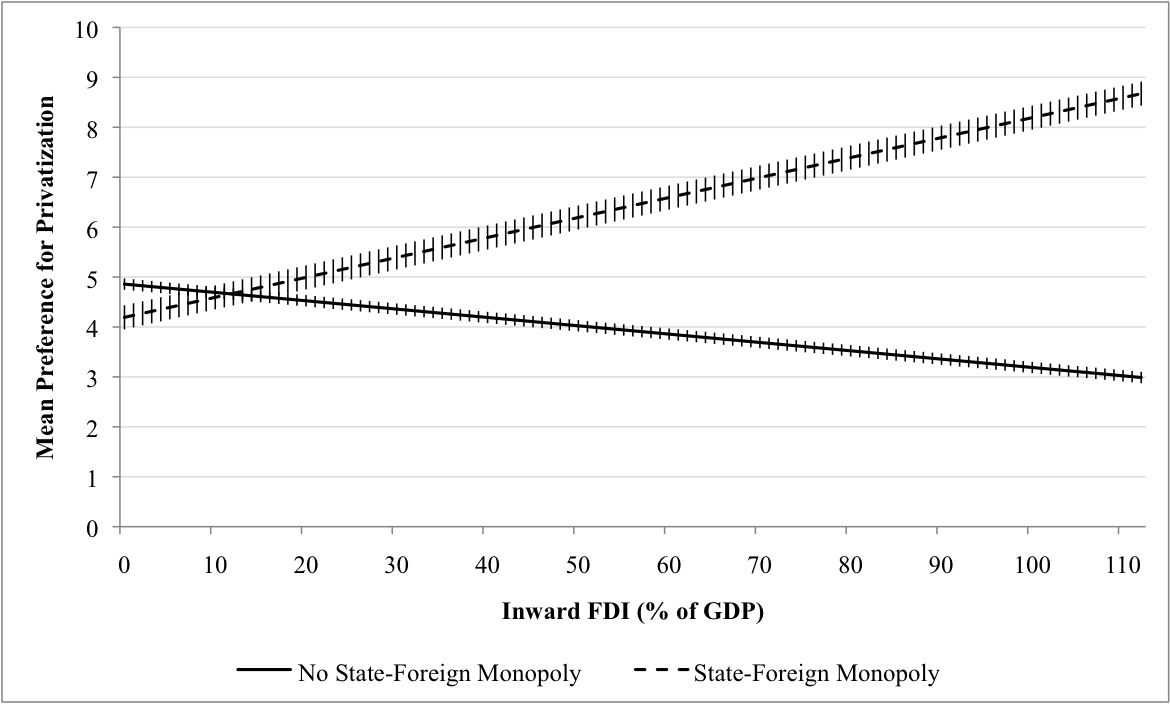
\includegraphics[scale=.75]{article3_fdi.png}
\caption{{Inward FDI (\% of GDP) and Expected Preference for Privatization}}
\end{center}
\end{figure}

\begin{figure}[htbp]
\begin{center}
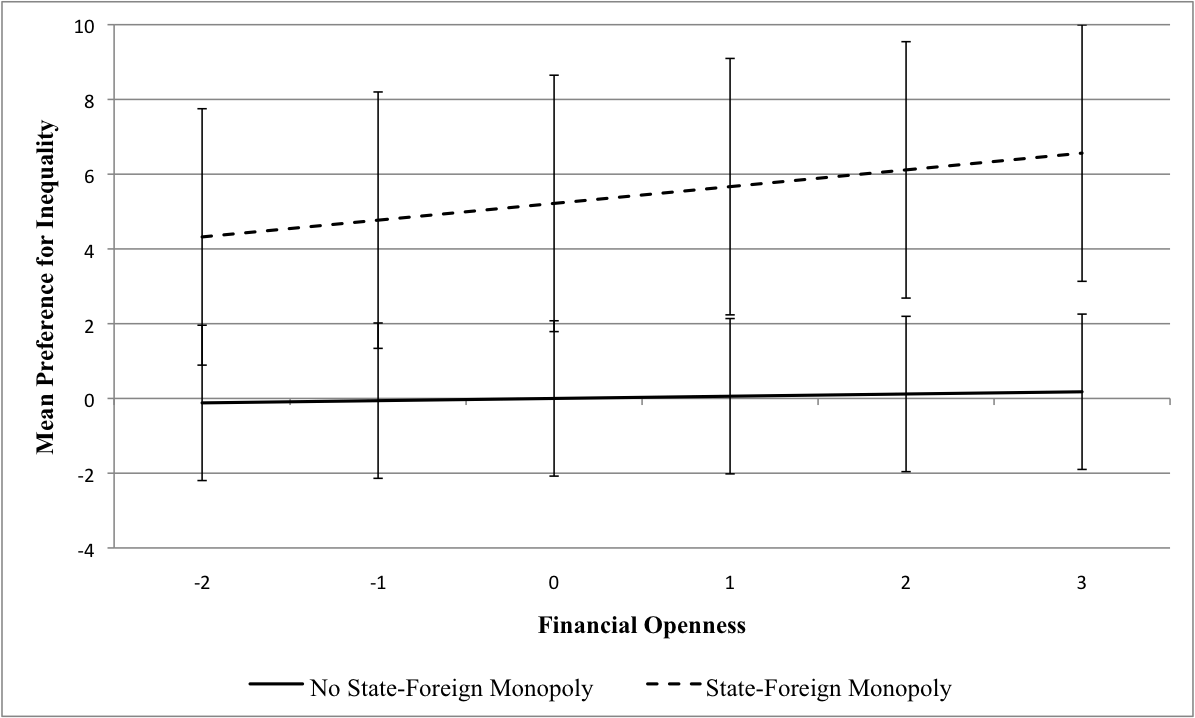
\includegraphics[scale=.75]{article3_finopen.png}
\caption{{Financial Openness and Preference for Inequality}}
\end{center}
\end{figure}

Perhaps most interestingly, when the media is dominated by the state or foreign companies, the effect of
globalization on attitudes is significant and as predicted in two cases. For instance, other things
equal, people prefer less privatization as foreign direct investment enters their country; when
there is a duopoly between the state and foreign companies, actors who have common biases against
the costs of globalization, then foreign-direct investment flows increase the desire for
privatization. We find the same reversal with respect to the tolerance of inequality under financial
openness. Although capital mobility, other things equal, does not have a statistically significant
effect on the demand for reducing inequality, when mediated by a state-foreign media duopoly capital
mobility is associated with favorable views regarding inequality as an incentive. Interesting as
these findings are, this evidence in support of Hypothesis 2 are only two cases out of a total of
nine combinations of alternative measures. In six other interaction terms, there is no statistically
significant result and in one the relationship ($tradeXduop$) runs counter to Hypothesis 2. At least
within the sample, in five of the nine combinations the coefficient is larger than the non-
interacted globalization measures, as predicted, with state-foreign domination of the media
decreasing attitudes in support of goverment intervention.

	Trade is anomalous with respect to its non-interacted and interacted terms. Surpisingly, trade
	seems to correlate negatively with the demand for government intervention and positively when
	interacted with a state-foreign media duopoly.
	
	These findings require caution. It is well known that survey respondents are extremely sensitive
	to question wording. On the whole, these results are far from definitive proof that the link
	between global market exposure and demand for public support is significantly and consistently
	conditioned by media ownership. Neither is it definitive proof one way or the other regarding
	the micro-processes of the compensation thesis. But as a first interrogation of these links, the
	results are certainly sufficient to conclude that the assumptions of the compensation thesis
	require further investigation and should not be taken for granted as in the seminal works of the
	globalization-welfare literature. Second, although the results regarding the media as
	conditioning the reception of globalization are also mixed, there is at least modest evidence
	for this argument. For the same reasons these results should not be interpreted as conclusively
	disproving the compensation thesis, the mixed evidence regarding the media's conditional effect
	calls for more research on this hypothesis.
	 
     The results of secondary regressions, with country fixed-effects, controls for pure and impure
serial correlation, and disaggregated media ownership, are presented below. Woolridge's test for
serial correlation in panel data show that very likely serial correlation is a problem in each case
except for the models using attitudes toward inequality as the dependent variable (p = 0.0066 for
attitudes toward privatization; p = 0.0347 for attitudes toward responsibility). In the first of the
secondary regressions, we find evidence in favor of the compensation thesis (H1) and of media's
conditioning effect (H2). Independently, FDI significantly decreases attitudes favorable toward
privatization in two of three cases controlling for media ownership. Trade has a similar effect in
only one case, when foreign ownership is controlled for. Financial openness never has the effect
predicted by the compensation thesis. The interaction of FDI with media ownership is not significant
when we consider foreign ownership alone, but it is significant in the hypothesized direction when
we consider state ownership and the combined effects of foreign and state ownership. Conversely, the
interaction of trade and media ownership is not significant with respect to state ownership, but it
is significant with respect to foreign ownership and the combined measure.

\begin{table}[htdp]
\caption{Dependent Variable: Attitudes in Favor of Privatization}
\vspace{2em}
\begin{center}
{\scriptsize
\begin{tabular}{lccc} \hline  & (1) & (2) & (3) \\ VARIABLES & Foreign & State & Foreign +
State \\ \hline  & &
 &  \\ fdi & -0.05 &
-0.14* & -0.17* \\  & (0.050) &
(0.058) & (0.067) \\
ttrade & -0.12*** & -0.07 & -0.12 \\  & (0.034) &
(0.097) & (0.099) \\
finance & 0.06 & 0.46 & 0.94 \\  & (0.549) &
(1.351) & (1.158) \\
percentforeign & -73.94*** &  &  \\  & (21.927) &
 &  \\ fdiXforeign &
0.53 &  &  \\  & (0.359) &
 &  \\ tradeXforeign &
0.89* &  &  \\  & (0.364) &
 &  \\ financeXforeign &
1.97 &  &  \\  & (3.217) &
 &  \\ percentstate &  &
-31.32 &  \\  &  &
(20.004) &  \\ fdiXstate
&  & 0.79* &  \\  &  &
(0.330) &  \\
tradeXstate &  & 0.26 &  \\  &  &
(0.250) &  \\
financeXstate &  & 2.85 &  \\  &  &
(4.358) &  \\ percentown
&  &  & -39.64** \\  &  &
 & (14.150) \\ fdiXfs &
&  & 0.66** \\  &  &
 & (0.232) \\ tradeXfs &
&  & 0.40* \\  &  &
 & (0.201) \\ financeXfs
&  &  & -0.56 \\  &  &
 & (1.602) \\ lagpriv &
0.80*** & 0.75*** & 0.70*** \\  & (0.063) &
(0.134) & (0.097) \\
Constant & 15.47*** & 15.18 & 21.27** \\  & (3.022) &
(9.043) & (7.894) \\
 &  &  &
 \\ Observations & 30 & 30 & 30 \\ $R^2$ & 0.86 & 0.85 & 0.87
\\ Number of cntry & 10 & 10 & 10 \\  $Rho$ & -.07 & -.19 & -.18 \\ \hline
\multicolumn{4}{c}{ Standard errors in parentheses.} \\
\multicolumn{4}{c}{ *** p$<$0.001, ** p$<$0.01, * p$<$0.05} \\
\multicolumn{4}{c}{ Coefficients for country fixed-effects are not displayed.
} \\

\end{tabular}
}
\end{center}
\label{default}
\end{table}


\begin{table}[htdp]
\caption{Dependent Variable: Attitudes in Favor of Inequality}
\vspace{2em}
\begin{center}
{\scriptsize
\begin{tabular}{lccc} \hline  & (1) & (2) & (3) \\ VARIABLES & Foreign &
State & Foreign+State \\ \hline  &  &
 &  \\ fdi & -0.18 &
-0.01 & -0.13 \\  & (0.122) &
(0.108) & (0.125) \\
ttrade & 0.11 & 0.07 & 0.09 \\  & (0.121) &
(0.073) & (0.109) \\
finance & 1.96** & 1.61* & 2.68*** \\  & (0.634) &
(0.630) & (0.659) \\
percentforeign & 23.39 &  &  \\  & (39.784) &
 &  \\ fdiXforeign &
0.38 &  &  \\  & (0.672) &
 &  \\ tradeXforeign &
-0.14 &  &  \\  & (0.687) &
 &  \\ financeXforeign &
-20.56*** &  &  \\  & (5.998) &
 &  \\ percentstate &  &
52.32 &  \\  &  &
(29.819) &  \\ fdiXstate
&  & -1.28 &  \\  &  &
(0.852) &  \\
tradeXstate &  & -0.47 &  \\  &  &
(0.351) &  \\
financeXstate &  & -13.79** &  \\  &  &
(5.093) &  \\ percentown
&  &  & 10.59 \\  &  &
 & (16.050) \\ fdiXfs &
&  & -0.08 \\  &  &
 & (0.406) \\ tradeXfs &
&  & -0.12 \\  &  &
 & (0.294) \\ financeXfs
&  &  & -8.14*** \\  &  &
 & (1.276) \\ lagineq &
0.19 & 0.03 & 0.08 \\  & (0.208) &
(0.180) & (0.184) \\
Constant & 40.80*** & 49.30*** & 46.47*** \\  & (11.870) &
(11.757) & (11.794) \\
 &  &  &
 \\ Observations & 30 & 30 & 30 \\ $R^2$ & 0.58 & 0.37 & 0.37
\\ Number of cntry & 10 & 10 & 10 \\  $Rho$ & -.15 & .12 & -.03 \\ \hline
\multicolumn{4}{c}{ Standard errors in parentheses} \\
\multicolumn{4}{c}{ *** p$<$0.001, ** p$<$0.01, * p$<$0.05} \\
\multicolumn{4}{c}{ Coefficients for country fixed-effects are not displayed.
} \\
\end{tabular}
} \end{center}
\label{default}
\end{table}

Results for attitudes toward inequality show no evidence in favor of either the compensation thesis
or the media interaction hypothesis. It is possible that attitudes towards whether the government
should intervene to lessen inequality reflect more than the demand for state intervention in
general, more so than attitudes toward privatization.

When using measures of attitudes toward personal versus government responsibility as the dependent
variable, we find evidence that FDI significantly decreases the attitude that people should be more
responsible, but evidence that trade either has no significant effect or it increases the belief in
personal responsibility in the case that we control for foreign media ownership. More interestingly,
we find evidence that state ownership and foreign plus state ownership significantly condition the
effect that FDI and trade have on attitudes toward who should be more responsible. Again, the
effects are in the predicted direction, with state ownership reversing the effect of two
globalization processes, from increasing the belief that the government should be more responsible
to increasing beliefs that individuals should be more responsible instead.


\begin{table}[htdp]
\caption{Dependent Variable: Attitudes in Favor of Personal Responsibility}
\vspace{2em}
\begin{center}
{\scriptsize
\begin{tabular}{lccc} \hline  & (1) & (2) & (3) \\ VARIABLES &
Foreign & State & Foreign+State \\ \hline  &  &
 &  \\ fdi & -0.19* &
-0.34*** & -0.22** \\  & (0.087) &
(0.060) & (0.082) \\
ttrade & 0.21* & 0.12 & 0.08 \\  & (0.095) &
(0.096) & (0.122) \\
finance & 0.91 & 2.82*** & 2.03* \\  & (0.551) &
(0.573) & (0.796) \\
percentforeign & -37.50 &  &  \\  & (36.474) &
 &  \\ fdiXforeign &
1.00 &  &  \\  & (0.573) &
 &  \\ tradeXforeign &
0.17 &  &  \\  & (0.654) &
 &  \\ financeXforeign &
-4.16 &  &  \\  & (4.048) &
 &  \\ percentstate &  &
-101.88*** &  \\  &  &
(28.788) &  \\ fdiXstate
&  & 1.96** &  \\  &  &
(0.621) &  \\
tradeXstate &  & 0.80** &  \\  &  &
(0.298) &  \\
financeXstate &  & -9.90** &  \\  &  &
(3.775) &  \\ percentown
&  &  & -52.40** \\  &  &
 & (17.727) \\ fdiXfs &
&  & 0.82** \\  &  &
 & (0.296) \\ tradeXfs &
&  & 0.57* \\  &  &
 & (0.280) \\ financeXfs
&  &  & -4.58* \\  &  &
 & (2.096) \\ lagresp &
0.71*** & 0.29 & 0.55*** \\  & (0.142) &
(0.153) & (0.105) \\
Constant & 7.89 & 32.69*** & 21.10*** \\  & (4.789) &
(9.112) & (5.687) \\
 &  &  &
 \\ Observations & 30 & 30 & 30 \\ $R^2$ & 0.60 & 0.62 & 0.75
\\ Number of cntry & 10 & 10 & 10 \\  $Rho$ & -.08 & -.01 & -.19 \\ \hline
\multicolumn{4}{c}{ Standard errors in parentheses} \\
\multicolumn{4}{c}{ *** p$<$0.001, ** p$<$0.01, * p$<$0.05} \\
\multicolumn{4}{c}{ Coefficients for country fixed-effects are not displayed.
} \\ \end{tabular}
} \end{center}
\label{default}
\end{table}

\pagebreak

\subsection{A Quantitative Analysis of Independent News LTD} Reported below are the regression
results analyzing the relationship between globalizing processes and mentions of globalization in 12
INL newspapers before and after their purchase by foreign-owned John Fairfax Holdings. The variable
of interest is the first variable reported, the interaction term representing New Zealand trade
filtered through Fairfax ownership. The significant and negatively signed coefficient suggests that
under Fairfax, the papers' reportage of globalization was significantly less an increasing function
of New Zealand trade than before Fairfax.

\begin{center}
\begin{table}
\caption{Multiple Regression with Panel-Corrected Standard Errors}
\vspace{2em}
{\scriptsize
\begin{tabular}{lc} \hline  &  \\ Independent Variables & Coefficient \\
\hline  &  \\ tradeXfairfax & -110.45* \\
 & (43.945) \\ nztrade & 135.36*** \\ 
& (21.069) \\ fairfax & 67.55** \\  &
(25.692) \\ wtrade & -0.00 \\  &
(0.000) \\ fdi & -13.98 \\  &
(16.475) \\ thailand & -4.69** \\  &
(1.708) \\ asean & 0.09 \\  &
(3.405) \\ china & -2.30 \\  &
(2.661) \\ singapore & -8.58*** \\  &
(1.970) \\ lag & 0.25* \\  &
(2.258) \\ Constant & -67.82*** \\  &
(12.599) \\  &
 \\ Observations & 153 \\ Number of newspapers & 12 \\ $R^2$ &
0.86 \\  Adj. $R^2$ & . \\ \hline \multicolumn{2}{c}{ Includes fixed effects by
newspaper. } \\ \multicolumn{2}{c}{ *** p$<$0.001, **
p$<$0.01, * p$<$0.05} \\
\end{tabular}
}
\label{default}
\end{table}
\end{center}

This is evidence in favor of the foreign-ownership part of Hypothesis 3, namely that the bias of
foreign-ownership is likely to imply a functional disconnect between real-world, national economic
integration in the global economy and reportage of globalization. Graphically, it is easy to observe
that when one runs separate regressions for the years 1995-2003 and 2003-2009, the slope is
significantly steeper and there is less standard error in the first period. The graph is only
interesting descriptively because the confidence intervals are inflated by separating the data into
two samples and running two separate regressions. The significance of the interaction term in the
full model shows that the difference is significant. I argue that this is modest evidence in favor
of the hypothesis that foreign-owned media outlets are likely to be biased toward globalization in a
way that represents it in a way disconnected from the real, lived experiences of a particular
national public.

\begin{center}
\begin{figure}[htbp]
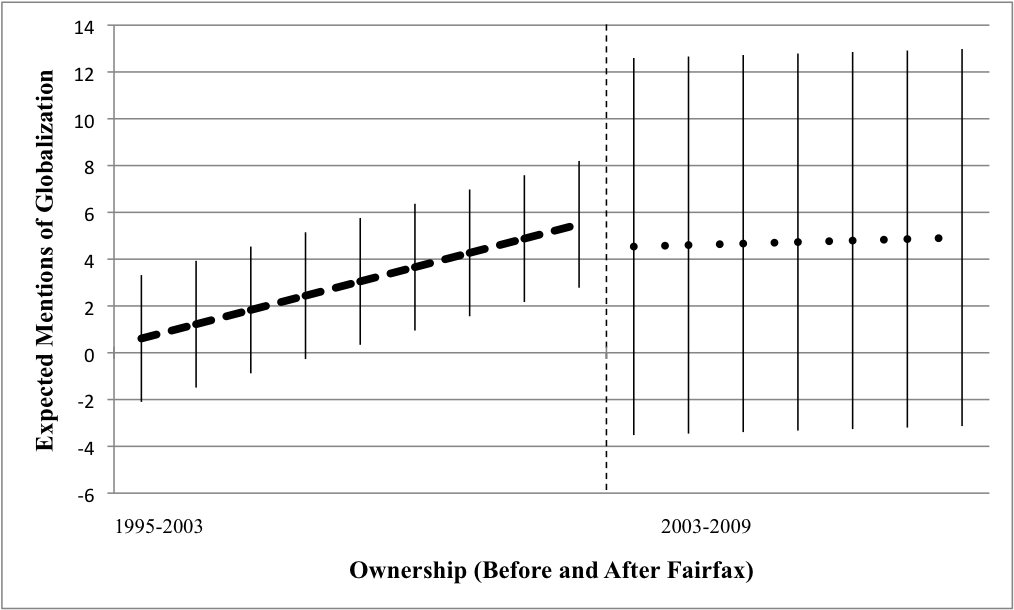
\includegraphics[scale=.85]{article3_rdgraph.png}
\caption{Discontinuous Regressions for Reportage of  Globalization and New Zealand Trade, 1995-2009}
\end{figure}
\end{center}

\subsection{A Qualitative Comparison of Media Representations}

To begin analysis of the actual social construction of globalization, consider the following table
which summarizes total number of news stories reporting on two major FTAs signed by New Zealand in
the past decade. Content analysis of newspaper reports in these time spans considered an article to
be "negative/debatable" if it mentioned any viewpoint critical of globalization or if it mentioned
that globalization is debated. Immediately, one notices that in the year leading up to an agreement,
the year of an agreement, and the year after an agreement, news reports under Fairfax are relatively
few, late, and uncritical.

\begin{center}
\begin{table}[htdp]
\caption{Comparison of TPSEP and NZSCEP Media Reports}
\vspace{2em}
\begin{center}
{\scriptsize
\begin{tabular}{lcccc} \hline & $T_{-1}$ &  $T$ &  $T_{+1}$ &
Total \\ \hline &  &  &
 \\ \bf{TPSEP} & & & &\\ Yearly Total & 0 & 0 & 3 & 3\\ \#
Negative/Debatable & 0 & 0 & 0 & 0  \\ \bf{NZSCEP} & & & & \\ Yearly Total & 0 & 7 & 1 &
8\\ \# Negative/Debatable & 0 & 6 & 1 & 7 \vspace{10pt}\\
\end{tabular}
}
\end{center}
\label{default}
\end{table}
\end{center}


More specifically, content analysis reveals the following distinct pattern of representation. After
2003, one finds in the pages of INL newspapers a \emph{naturalization} of globalization. In the
reports on the 2001 NZSCEP, globalization is a political phenomenon with proponents and critics
debating the issue. For instance, six of the reports are ``Day in the House" articles reporting that
the legislature was actively reviewing and debating the proposed NZSCEP. The NZSCEP is an uncertain
prospect with costs and benefits, as well as proponents (Labour and National parties) and opponents
(Alliance and Green parties) (Evening Post, Nov. 16, 2000). In contrast, after 2006, in the three
stories reporting on the TPSEP, it is striking that in each case, the defining problematic which
makes the story newsworthy is that New Zealand is suffering in one way or another from \emph{not
enough} free trade. (Dominion Post 2006; Timaru Herald 2006; The Press 2006). A representative
example is the second sentence in the 2006 article from \emph{The Press}, which is supposed to
capture the interest of the reader with "growing fears New Zealand may be losing out in the race to
clinch bilateral deals to remove trade barriers such as tariffs and quotas." Noticeably, Lexis-Nexis
finds zero "Day in the House" articles such as those that represented the NZSCEP as a legislative
debate. In 2006, globalization becomes a given, something that \emph{happened}. Thus, a strikingly
noticeable qualitative difference in the social construction of globalization emerges after a shift
toward foreign ownership: globalizing free-trade agreements that were previously represented as
contentious, debatable, prospective political issues become already decided, hardly arguable, given
or naturalized facts.


\section{Conclusion}

To conclude, I find mixed but suggestive evidence, from three levels of analysis, that media
ownership significantly conditions the political response of mass publics toward globalization. The
main quantitative analysis reveal that the assumptions of the compensation thesis are problematic:
in relatively few of the different model specifications examining different measures of
globalization and different attitudes toward government intervention was there significant evidence
that people demand government intervention to compensate for exposure to global free trade. In
relatively few cases was the sign of the coefficient even as predicted by this thesis. The main
findings of interest, and the main potential contribution of this paper, relate to the effect of
media ownership in mediating the political response to exposure to global free trade. Although
findings were not consistent and were very sensitive to model specification, more than half of the
total cross-national models showed that either foreign or state ownership significantly dampened or
reversed the effect of some globalization process on some attitude toward the demand for state
intervention. Given the shortcomings of the data, I interpret the sum of the findings as a promising
warrant for more research on this question. In short, the findings problematize accepted wisdom and
provide a suggestive first cut at a fairly new, fairly bold hypothesis. The within-case quantitative
and qualitative evidence further suggest that media ownership significantly determines bias in the
social construction of globalization.


\section{Appendix}

\begin{table}[htdp]
\caption{Appendix: Countries in Main Quantitative Analysis}
\begin{center}
\vspace{2em}
\begin{tabular}{ccc}
Albania & Algeria & Argentina \\ \\
Armenia & Australia & Azerbaijian \\ \\
Bangladesh & Belarus & Belgium \\ \\
Bosnia Herzegovina & Brazil & Bulgaria \\ \\
Canada & Chile & China \\ \\
Colombia & Croatia & Czech Republic \\ \\
Dominican Republic & Egypt & El Salvador \\ \\
Estonia & Finland & France \\ \\
Georgia & Ghana & Guatemala \\ \\
Hungary & Iceland & India \\ \\
Ireland & Italy & Japan \\ \\
Korea & Mexico & Netherlands \\ \\
New Zealand & Norway & Poland \\ \\
Slovenia & Spain & Sweden \\ \\
Switzerland & Turkey & United Kingdom \\ \\
United States & Venezuela \\ \\

\end{tabular}
\end{center}
\label{default}
\end{table}


\bibliographystyle{apsr2006}

\bibliography{mybib}

\end{document}
